% -*- Mode:TeX -*-

%% IMPORTANT: The official thesis specifications are available at:
%%            http://libraries.mit.edu/archives/thesis-specs/
%%
%%            Please verify your thesis' formatting and copyright
%%            assignment before submission.  If you notice any
%%            discrepancies between these templates and the 
%%            MIT Libraries' specs, please let us know
%%            by e-mailing thesis@mit.edu

%% The documentclass options along with the pagestyle can be used to generate
%% a technical report, a draft copy, or a regular thesis.  You may need to
%% re-specify the pagestyle after you \include  cover.tex.  For more
%% information, see the first few lines of mitthesis.cls. 

%\documentclass[12pt,vi,twoside]{mitthesis}
%%
%%  If you want your thesis copyright to you instead of MIT, use the
%%  ``vi'' option, as above.
%%
%\documentclass[12pt,twoside,leftblank]{mitthesis}
%%
%% If you want blank pages before new chapters to be labelled ``This
%% Page Intentionally Left Blank'', use the ``leftblank'' option, as
%% above. 

\documentclass[11pt,singlespace,leftblank]{mitthesis}
%\documentclass[12pt,twoside]{mitthesis}
\usepackage{lgrind}
%% These have been added at the request of the MIT Libraries, because
%% some PDF conversions mess up the ligatures.  -LB, 1/22/2014
\usepackage{cmap}
\usepackage[T1]{fontenc}
\pagestyle{plain}

%% This bit allows you to either specify only the files which you wish to
%% process, or `all' to process all files which you \include.
%% Krishna Sethuraman (1990).

% BEGIN MGymrek specific styles
\usepackage{adjustbox}
\usepackage{amsmath}
\usepackage{color}
\usepackage{geometry}
\usepackage{graphicx}
\usepackage{hyperref}
\usepackage{parskip}
\usepackage{setspace}
\usepackage{titlesec}

% For horizontal lines
\newcommand{\hzline}{\noindent\rule[0.5ex]{\linewidth}{1pt}}

% Paragraph spacing
\setlength{\parindent}{0em}
\setlength{\parskip}{0.5em}

% Default font
\renewcommand*{\familydefault}{\sfdefault}

% Chapter title pages
\titleformat{\chapter}[display]
    {\normalfont\huge\bfseries}{\chaptertitlename\ \thechapter}{20pt}{\Large}
\titlespacing*{\chapter}{0pt}{0pt}{20pt}
\onehalfspacing

% hyperlinks
\hypersetup{
  breaklinks=true,  % so long urls are correctly broken across lines
  colorlinks=true,
  urlcolor=blue,
  linkcolor=black,
  citecolor=red,
 }

% END MGymrek specific styles

%\typein [\files]{all}
%\def\all{all}
%\ifx\files\all \typeout{Including all files.} \else \typeout{Including only \files.} \includeonly{\files} \fi

\begin{document}

% -*-latex-*-
% 
% For questions, comments, concerns or complaints:
% thesis@mit.edu
% 
%
% $Log: cover.tex,v $
% Revision 1.8  2008/05/13 15:02:15  jdreed
% Degree month is June, not May.  Added note about prevdegrees.
% Arthur Smith's title updated
%
% Revision 1.7  2001/02/08 18:53:16  boojum
% changed some \newpages to \cleardoublepages
%
% Revision 1.6  1999/10/21 14:49:31  boojum
% changed comment referring to documentstyle
%
% Revision 1.5  1999/10/21 14:39:04  boojum
% *** empty log message ***
%
% Revision 1.4  1997/04/18  17:54:10  othomas
% added page numbers on abstract and cover, and made 1 abstract
% page the default rather than 2.  (anne hunter tells me this
% is the new institute standard.)
%
% Revision 1.4  1997/04/18  17:54:10  othomas
% added page numbers on abstract and cover, and made 1 abstract
% page the default rather than 2.  (anne hunter tells me this
% is the new institute standard.)
%
% Revision 1.3  93/05/17  17:06:29  starflt
% Added acknowledgements section (suggested by tompalka)
% 
% Revision 1.2  92/04/22  13:13:13  epeisach
% Fixes for 1991 course 6 requirements
% Phrase "and to grant others the right to do so" has been added to 
% permission clause
% Second copy of abstract is not counted as separate pages so numbering works
% out
% 
% Revision 1.1  92/04/22  13:08:20  epeisach

% NOTE:
% These templates make an effort to conform to the MIT Thesis specifications,
% however the specifications can change.  We recommend that you verify the
% layout of your title page with your thesis advisor and/or the MIT 
% Libraries before printing your final copy.
% TODO edit title
\title{Characterizing variation at short tandem repeats and their role in human genome regulation}

\author{Melissa A. Gymrek}
% If you wish to list your previous degrees on the cover page, use the 
% previous degrees command:
%       \prevdegrees{A.A., Harvard University (1985)}
% You can use the \\ command to list multiple previous degrees
%       \prevdegrees{B.S., University of California (1978) \\
%                    S.M., Massachusetts Institute of Technology (1981)}
\prevdegrees{B.S. in Computer Science and Engineering and in Mathematics, Massachusetts Institute of Technology (2011)}
\department{Harvard-MIT Program in Health Sciences and Technology}

% If the thesis is for two degrees simultaneously, list them both
% separated by \and like this:
% \degree{Doctor of Philosophy \and Master of Science}
\degree{Doctor of Philosophy}

% As of the 2007-08 academic year, valid degree months are September, 
% February, or June.  The default is June.
\degreemonth{June} % TODO
\degreeyear{2016}
\thesisdate{February 1, 2016} % TODO

%% By default, the thesis will be copyrighted to MIT.  If you need to copyright
%% the thesis to yourself, just specify the `vi' documentclass option.  If for
%% some reason you want to exactly specify the copyright notice text, you can
%% use the \copyrightnoticetext command.  
%\copyrightnoticetext{\copyright IBM, 1990.  Do not open till Xmas.}

% If there is more than one supervisor, use the \supervisor command
% once for each.
\supervisor{Yaniv Erlich, PhD}{Assistant Professor of Computer Science, Columbia University}
\supervisor{Mark J. Daly, PhD}{Associate Professor Medicine, Harvard Medical School}

% This is the department committee chairman, not the thesis committee
% chairman.  You should replace this with your Department's Committee
% Chairman.
\chairman{Emery N. Brown, MD, PhD}{Director, Harvard-MIT Program in Health Sciences and Technology/Professor of Computational Neuroscience and Health Sciences and Technology}

% Make the titlepage based on the above information.  If you need
% something special and can't use the standard form, you can specify
% the exact text of the titlepage yourself.  Put it in a titlepage
% environment and leave blank lines where you want vertical space.
% The spaces will be adjusted to fill the entire page.  The dotted
% lines for the signatures are made with the \signature command.
\maketitle

% The abstractpage environment sets up everything on the page except
% the text itself.  The title and other header material are put at the
% top of the page, and the supervisors are listed at the bottom.  A
% new page is begun both before and after.  Of course, an abstract may
% be more than one page itself.  If you need more control over the
% format of the page, you can use the abstract environment, which puts
% the word "Abstract" at the beginning and single spaces its text.

%% You can either \input (*not* \include) your abstract file, or you can put
%% the text of the abstract directly between the \begin{abstractpage} and
%% \end{abstractpage} commands.

% First copy: start a new page, and save the page number.
\cleardoublepage
% Uncomment the next line if you do NOT want a page number on your
% abstract and acknowledgments pages.
% \pagestyle{empty}
\setcounter{savepage}{\thepage}
\begin{abstractpage}
% $Log: abstract.tex,v $
% Revision 1.1  93/05/14  14:56:25  starflt
% Initial revision
% 
% Revision 1.1  90/05/04  10:41:01  lwvanels
% Initial revision
% 
%
%% The text of your abstract and nothing else (other than comments) goes here.
%% It will be single-spaced and the rest of the text that is supposed to go on
%% the abstract page will be generated by the abstractpage environment.  This
%% file should be \input (not \include 'd) from cover.tex.
% TODO pasted from CSHL abstract. edit this for here! 350 words, outline:

A central goal in genomics is to understand the genetic variants that underlie molecular changes and lead to disease. Recent studies have identified thousands of genetic loci associated with human phenotypes. These have primarily analyzed point mutations, ignoring more complex types of variation. Here we focus on Short Tandem Repeats (STRs) as a model for complex variation. STRs are comprised of repeating motifs of 1-6bp that span over 1\% of the human genome. The level of STR variation and its effect on phenotypes remains mostly uncharted, mainly due to the difficulty in accurately genotyping STRs on a large scale.

To overcome bioinformatic challenges in high throughput STR genotyping, we developed lobSTR, an algorithm for profiling STRs from high throughput sequencing data. lobSTR employs a unique mapping strategy to rapidly align repetitive reads, and uses statistical learning techniques to account for STR-specific noise patterns. We applied lobSTR to generate the largest and highest quality STR catalog to date. This provided the first characterization of more than a million loci and gave novel insights into population-wide trends of STR variation. We used this catalog to conduct a genome-wide analysis of the contribution of STRs to gene expression in humans. This revelated that STRs explain 10-15\% of the \emph{cis} heritability of expression mediated by common variants and potentially play a role in various clinically relevant conditions.

Overall these studies highlight the contribution of STRs to the genetic architecture of quantitative traits. We anticipate that integrating the analysis of repetitive elements, specifically STRs, will lead to the discovery of new genetic variants relevant to human conditions.
\end{abstractpage}

% Additional copy: start a new page, and reset the page number.  This way,
% the second copy of the abstract is not counted as separate pages.
% Uncomment the next 6 lines if you need two copies of the abstract
% page.
% \setcounter{page}{\thesavepage}
% \begin{abstractpage}
% % $Log: abstract.tex,v $
% Revision 1.1  93/05/14  14:56:25  starflt
% Initial revision
% 
% Revision 1.1  90/05/04  10:41:01  lwvanels
% Initial revision
% 
%
%% The text of your abstract and nothing else (other than comments) goes here.
%% It will be single-spaced and the rest of the text that is supposed to go on
%% the abstract page will be generated by the abstractpage environment.  This
%% file should be \input (not \include 'd) from cover.tex.
% TODO pasted from CSHL abstract. edit this for here! 350 words, outline:

A central goal in genomics is to understand the genetic variants that underlie molecular changes and lead to disease. Recent studies have identified thousands of genetic loci associated with human phenotypes. These have primarily analyzed point mutations, ignoring more complex types of variation. Here we focus on Short Tandem Repeats (STRs) as a model for complex variation. STRs are comprised of repeating motifs of 1-6bp that span over 1\% of the human genome. The level of STR variation and its effect on phenotypes remains mostly uncharted, mainly due to the difficulty in accurately genotyping STRs on a large scale.

To overcome bioinformatic challenges in high throughput STR genotyping, we developed lobSTR, an algorithm for profiling STRs from high throughput sequencing data. lobSTR employs a unique mapping strategy to rapidly align repetitive reads, and uses statistical learning techniques to account for STR-specific noise patterns. We applied lobSTR to generate the largest and highest quality STR catalog to date. This provided the first characterization of more than a million loci and gave novel insights into population-wide trends of STR variation. We used this catalog to conduct a genome-wide analysis of the contribution of STRs to gene expression in humans. This revelated that STRs explain 10-15\% of the \emph{cis} heritability of expression mediated by common variants and potentially play a role in various clinically relevant conditions.

Overall these studies highlight the contribution of STRs to the genetic architecture of quantitative traits. We anticipate that integrating the analysis of repetitive elements, specifically STRs, will lead to the discovery of new genetic variants relevant to human conditions.
% \end{abstractpage}

\cleardoublepage

%%%%%%%%%%%%%%%%%%%%%%%%%%%%%%%%%%%%%%%%%%%%%%%%%%%%%%%%%%%%%%%%%%%%%%
% -*-latex-*-

% Some departments (e.g. 5) require an additional signature page.  See
% signature.tex for more information and uncomment the following line if
% applicable.

\pagestyle{plain}
  % -*- Mode:TeX -*-
%% This file simply contains the commands that actually generate the table of
%% contents and lists of figures and tables.  You can omit any or all of
%% these files by simply taking out the appropriate command.  For more
%% information on these files, see appendix C.3.3 of the LaTeX manual. 
\tableofcontents
%\newpage
%\listoffigures
%\newpage
%\listoftables


\onehalfspacing
\iffalse \bibliography{MGymrekRefs.bib} \fi

\chapter{Introduction}

\section{Overview}

% Goal of genomics
A central goal in genomics is to understand the genetic variants that underlie phenotypic changes and lead to disease. Recent studies have identified thousands of genetic loci associated with human phenotypes. Since the advent of next generation sequencing, the majority of genomic studies have focused on single nucleotide polymorphisms (SNPs). These are both the simplest type of variation to genotype and one of the easiest to model. However, a wide range of other classes of variants is important for controlling phenotypes.

% STRs as a model
Short tandem repeats (STRs) consist of period DNA motifs of 1-6bp and comprise of more than 1\% of the human genome. Their repetitive structure induces DNA polymerase slippage events that add or delete repeat units, resulting in mutation rates that are orders of magnitude higher than those for most other variant types. STRs are implicated in more than 40 human diseases, mostly consisting of Mendelian disorders caused by large expansions of trinucleotide repeats. Additionally, several dozen single gene studies have shown that STRs can be involved in quantitative traits including gene expression. Because of their abundance, high polymorphism rates, and previous implication of functional roles, we focused on STRs as a model to investigate the role of complex variants in human phenotypes.

% What I present as our contribution
Here I present our contributions to enable the first large scale studies of STR variation and reveal that these loci play a significant role in complex traits in humans. In the first part of this thesis, we develop novel tools for high-throughput STR analysis from next generation sequencing data (\textbf{\autoref{chap:lobstr}, \autoref{chap:pbv}}). We then apply these methods to large sequencing cohorts consisting of thousands of samples with diverse origins to provide the first population-wide catalog of hundreds of thousands of previously uncharacterized STR loci (\textbf{\autoref{chap:catalog}, \autoref{chap:sgdp}}). An important aspect of this work has been a commitment to maximize utility of our results for the wider genomics community through providing open-source software packages and online visualization tools that are alredy being utilized by other researchers. In the second part of this thesis, we interrogate the role of STRs in complex traits, focusing on gene expression as an initial phenotype (\textbf{\autoref{chap:estr}}). This study reveals more than 2,000 STRs whose lengths are correlated with gene expression (termed ``expression STRs'', or eSTRs) and shows that STRs make a significant contribution to regulating expression of nearby genes. These loci are enriched in putative regulatory regions and are predicted to modulate regulatory activity. These results highlight the contribution of STRs to the genetic architecture of gene expression and complex traits in humans.

% To frame this work
To frame this work, I first review properties and applications of STRs and what we know about their contribution to disease and molecular phenotypes in humans. Next, I describe challenges in developing high throughput methods for STR analysis and state of the art experimental and bioinformatic methods for doing so. I summarize what we have learned to date about patterns of STR variation in humans using these methods. Then, I review what has been revealed about the genetic architecture of gene expression through SNP studies and the contribution of gene regulation to human conditons. I examine evidence that suggests variants such as STRs that are not well tagged by common SNPs may play an important role in these traits. Finally, I summarize the contributions of this thesis toward enabling large scale STR analysis and highlighting an important role fo STRs in human phenotypes.

\section{STRs are abundant in the human genome}
intro: define STRs, genome composition
\subsection{Genome-wide composition of STRs}
\subsection{Applications of STRs}
forensics, genealogy, linkage analysis
\subsection{Processes leading to STR variation}

\section{Evidence from model organisms of a regulatory role for STRs}
% TODO - specific examples
% TODO - comparative

\section{STRs in human disease and phenotypic variation}
Dozens of STRs have been implicated in both disease and molecular phenotypes in humans. In nearly all of these cases, the resulting phenotype showed a quantitative relationship with the number of repeats, strongly suggesting STRs may play an important role in complex traits.

\subsection{Dozens of disorders are caused by STR expansions}
% intro, examples
STR expansions are known to cause dozens of human single-gene, Mendelian disorders \cite{Mirkin2007}, affecting more than hundreds of thousands of patients in the U.S. \cite{CoffeeKeithAlbizuaEtAl2009}. The majority of these are due to expansions of trinucleotide repeats, and nearly all affect neurological function, most with a late onset disease course. For instance, an exonic CAG repeat expansion encoding polyglutamine results in Huntington's Disease, a devastating neurological disorder \cite{Mirkin2007}; CGG expansion disrupts a methylation site on the X chrmosome leading to Fragile X Syndrome, one of the leading cuases of mental retardation in males \cite{LyonLaverYuEtAl2010}; a CUG expansion in the 3' untranslated (UTR) region \emph{DPMK} results in myotonic dystrophy \cite{BrookMcCurrachHarleyEtAl1992}, a severe multisystemic form of muscular dystrophy. 
Other classes of repeats have been implicated in STR expansion diseases. Recently, high throughput sequencing scans for causative SNPs fortuitously revealed that a hexanucleotide expansion in \emph{C9orf72} is responsible for 9p21-linked amyotrophic lateral sclerosis-frontotemporal dementia (ALS-FTD) \cite{RentonMajounieWaiteEtAl}. A summary of STR expansion diseases is given by Mirkin \cite{Mirkin2007}. %shown in \textbf{Table \ref{tab:intro1}}.

% TODO complete table
%\begin{table}[h!]
%\label{tab:intro1}
%\centering
%\begin{tabular}{c c c c c c}
%\hline
%Disorder & Gene & Repeat & Normal range & Pathogenic range & References \\
%\hline
%\hline
%\end{tabular}
%\caption{\textbf{An overview of STR expansion disorders.}}
%\end{table}

% mechanism?
The mechanisms by which most of these expansions lead to disease are still poorly understood. In cases of exonic repeat expansions, particularly polyglutamine expansions such as Huntington's Disease, it is thought that the expanded amino acid tracts form toxic aggregates that accumulate over time, consistent with the late-onset nature of these diseases \cite{MichalikVanBroeckhoven2003}. Alternatively, it was recently shown that a key factor in Huntington's Disease may be repeat-length dependent aberrant splicing of \emph{HTT} \cite{SathasivamNeuederGipsonEtAl2013}. Other proposed pathogenic mechanisms include loss of protein expression, over-expression of the wildtype protein copy, and toxic gain of function of RNAs encoding expanded repeats \cite{Pearson2011}. Recent studies have found evidence that an alternative mechanism, ``Repeat-associated non-ATG translation'', termed ``RAN-translation'', may be responsible for rendering CAG repeats toxic. Under this phenomenon, expanded CAG repeats in RNA may be translated in the absence of an ATG start codon, and may produce transcripts under all seven possible reading frames \cite{Pearson2011}. These ``RAN'' transcripts have already been identified in patients with a variety of repeat disorders, including spinocerebellar ataxia type 8 (SCA8), myotonic dystrophy type 1 (DM1), Fragile-X tremor ataxia syndrome (FXTAS), and ALS-FTD \cite{ClearyRanum2014}.

% anticipation, correlation with repeat number
One hallmark of repeat disorders is the phenomenon of ``anticipation'' in which the severity of the condition tends to increase and the age of onset tends to decrease with each generation. This generally corresponds to an in increase in repeat number for the expanded allele in each generation. Many of these repeats, experience a bi-phasic mutation process: under a certain number of repeats the region is stable with relatively low mutation rate. However, once a threshold length has been passed, the repeat will have an extremely high mutation rate and tend toward massive expansions \cite{BourgeoisCoffeyRiveraEtAl2009}. In many cases, the number of repeats is directly related to phenotype. For instance, there is a negative linear relationship between CAG repeat number and age of onset of Huntington's Disease \cite{Rubinsztein2002}. Interestingly, this suggests that unlike point mutations, which can serve as an ``on/off'' switch for Mendelian and other disorders, repeats possess a more fine-tunable mechanism to affect phenotype by adjusting the number of repeats on a quantitative, rather than a binary, scale.

% polymorphism in population 
Many such pathogenic STR expansions have been characterized, clearly indicating a biological function for at least a subset of repetitive elements. However, the majority of repeats remain uncharacterized and little is known about the extent of polymorphism and allele ranges at these and other STRs in healthy individuals. As mentioned above, STRs are prone to replication slippage events that cause them to mutate rapdily. Whereas intermediate length STRs of $\sim<$200bp tend to mutate in a stepwise fashion. longer repeats such as those involved in expansion disorders may for unusual non-B DNA structures \cite{KozlowskiSobczakKrzyzosiak2010} that cause rapid expansions, leading to unusual behavior in pathogenic conditions. We hypothesize that whereas longer unstable repeats radically disrupt function of a given locus, leading to severe mono-genic disorders, STRs in the intermediate range length may be responsible for fine-tuning genomic regulation and for contributing to more incremental variation, which could make an important contribution to more complex traits in humans.

\subsection{STRs in complex human traits}
Little is known about the role of STRs in more complex, polygenic traits. This is largely due to the fact that until recently there was limited ability to systematically profile these loci on a large scale (see \ref{sec:intromethods}) and because SNP-based studies have limited ability to capture STR associations (see \ref{sec:introarch}). However, a small number of STR associations with complex traits have been reported: repeat length in the first exon of the androgen receptor correlates with risk of hepatocellular carcinoma risk in women \cite{YuYangYangEtAl2002}; a TC repeat in \emph{HMGA2} is associated with uterine leiomyomata and decreased height \cite{HodgeTCuencoHuyckEtAl2009}; a CAG repeat in \emph{KCNN3} is associated with cognitive performance in schizophrenia \cite{GrubeGerchenAdamcioEtAl2011}. However, no study has systematically evaluated the role of STRs in complex traits.

\subsection{Mechanisms for STR involvement in genome regulation}
STRs are found in at least 5\% of human protein-coding genes \cite{ODushlaineEdwardsParkEtAl2005} and are abundant in intragenic regions and UTRs \cite{LiKorolFahimaEtAl2004}. These rapidly evolving elements provide an evolutionary substrate to incrementally affect gene activity without introducing major sequences changes. STRs have been demonstrated or hypothesized to affect gene regulation in several ways, summarized below. % and in \textbf{Table \ref{tab:intro2}}.

\subsubsection{Transcribed STRs}
% exonic
As described above, many putative pathogenic STRs lie in coding regions and may lead to disease through mechanisms such as protein or RNA aggregation, RAN-translation, or aberrant splicing. Alternative mechanisms could allow exonic STRs to affect protin function. For instance, STR mutations in coding regions could function to silence genes by introducing frameshift mutations leading to premature stop codons \cite{GemayelVincesLegendreEtAl2010}, especially in the case of non tri- or hexa-nucleotide repeats. Additionally, expansions or contractions could alter spacing between protein domains, leading to a change in function.

% intronic
Intronic repeats may also affect gene regulation. Lengths of intronic STRs have been shown to affect gene expression \cite{GebhardtZankerBrandt1999}, in some cases through altering transcription factor binding sites. For example, a TATC repeat in \emph{TH} affects binding of the transcription factor ZNF191 \cite{AlbaneseBiguetKieferEtAl2001}. Several studies have also shown that intronic STRs may regulate splicing efficiency in a repeat-specific manner. For instance, the length of an intronic TG repeat in \emph{CFTR} is directly related with inclusion of the adjacent exon \cite{HefferonGromanYurkEtAl2004}, which is likely to be due to effects of the repeat on RNA secondary structure. An intronic CA repeat in \emph{eNOS} was shown to regulate splicing by affecting binding of the splicing factor HnRNP L \cite{HuiStanglLaneEtAl2003}, and it was later shown that intronic CA repeats may have a widespread effect on splicing \cite{HuiHungHeinerEtAl2005}.

% UTRs
Finally, STRs in UTRs may affect gene regulation. For example, a CTG/CAG repeat in the 3'UTR of \emph{DMPK} is implicated in the repeat expansion disorder myotonic dystrophy 1, and is thought to sequester splicing factors leading to aberrant splicing \cite{KoscianskaWitkosKozlowskaEtAl2015}. 3'UTR repeats may also harbor microRNA binding sites, affecting gene regulation.

\subsubsection{STR lengths influence promoter and enhancer activity}
In addition to transcribed regions, STRs can affect the function of genomic regulatory elements through several mechanisms. AC dinucleotides are over-represented in predicted \emph{cis}-regulatory elements \cite{RockmanWray2002}. Recently, it was shown that dinucleotide repeats are a hallmark of enhancer elements in \emph{Drosophila} and human cell lines \cite{Yanez-CunaArnoldStampfelEtAl2014}. This suggests they may provide an abundant source of transcriptional regulation in these elements. Heidari, \emph{et al.} \cite{HeidariNarimanSalehFamEsmaeilzadeh-GharehdaghiEtAl2012} demonstrated that a GA repeat in the promoter of \emph{SOX5} can affect nucleosome processing, affecting downstream gene expression. This finding is supported by a study in yeast that found variation in repeat length had a strong effect on nucleosome positioning and gene expression in 25 of 33 randomly chosen STR-containing promoters \cite{VincesLegendreCaldaraEtAl2009}. STRs may also bind transcription factors and create a number of binding sites dependent on the number of repeats. Guillon \emph{et al.} found that the oncogenic EWSR1-FLI1 fusion protein formed in Ewing Sarcoma preferentially binds GGAA repeats \cite{GuillonTirodeBoevaEtAl2009}. Interestingly, a recently study found that a reported genome-wide association study (GWAS) signal for Ewing Sarcoma actually points to a SNP for which the alternate allele joins two adjacent GGAA repeats into one long repeat tract, resulting in overexpression of the nearby gene \emph{EGR2} \cite{GrunewaldBernardGilardi-HebenstreitEtAl2015}. In another example, a pentanucleotide repeat in the promoter of \emph{PIG3} creates a varying number of \emph{p53} binding sites, affecting downstream expression \cite{ContenteDittmerKochEtAl2002}.

% TODO complete table
%\begin{table}[h!]
%\centering
%\label{tab:intro2}
%\begin{tabular}{c c c c c}
%\hline
%Gene & STR location & Tissue & Direction of effect & Reference \\
%\hline
%\hline
%\end{tabular}
%\caption{\textbf{STRs implicated in gene regulation. Full references given in the main text}}
%\end{table}

Together, these examples show clear evidence that STRs may regulate quantitative traits, such as gene expression, transcription factor binding, and splicing efficiency, in a repeat-dependent manner and therefore are prime candidates for contributing to complex traits in humans.

\section{Methods for genotyping STRs}
\label{sec:intromethods}
\subsection{Capillary electrophoresis}
The current gold standard technique for STR typing relies on cumbersome capillary electrophoresis methods \cite{ButlerBuelCrivellenteEtAl2004}, which require PCR amplification of the locus of interest, followed by size separation via electrophoresis to determine the alleles present. The method is widely used for typing STRs used as genetic markers for linkage analyses (Marshfield set \cite{BromanMurraySheffieldEtAl1998}), the FBI CODIS set, markers for genealogical studies \cite{ZerjalXueBertorelleEtAl2003,SkoreckiSeligBlazerEtAl1997} and for determining alleles present at known pathogenic loci \cite{LyonLaverYuEtAl2010,BlancoSuarezGandia-PlaEtAl2008}.

Capillary electrophoresis uses a separate reaction per locus, and requires time-consuming optimization of conditions for each reaction. With a cost that is upwards of several dollars per STR and lengthy preparation, current panels can consist of up to several hundreds of STRs - only a fraction of the hundreds of thousands of STR loci in the human genome \cite{Benson1999}. While the method is robust and can achieve accuracy above 99\% \cite{WeberBroman2001}, it has several technical limitations. First, many loci, especially dinucleotide STRs, are plagued by ``stutter peaks'' due to errors introduced during PCR amplification that may complicate calling. Second, this technique can only return the size of the allele: it is unable to distinguish homoplasmic alleles \cite{WeberBroman2001} (two different alleles with the same size but distinct sequences). Third, because capillary techniques simply return the length of the amplified region, it will be sensitive to the presence of linked insertions or deletions that are not part of the STR itself being genotyped. Due to these limitations, electrophoresis is unable to provide an accurate genome-wide picture of sequence variation at STR loci.

\subsection{Genotyping STRs from next-generation sequencing}
\subsubsection{Challenges of genotyping STRs from short reads}
Although theoretically any type of variation should be captured by DNA sequencing, STRs have proven challenging to genotype from short reads produced by high-throughput sequencing platforms. Major challenges include:
\begin{enumerate}
\item Reads must entirely span an STR region to be informative about the number of repeats present.
\item STRs with a large length difference from the reference sequence present as a gapped alignment problem. The run time of mainstream aligners such as BWA \cite{LiDurbin2009a} increases rapidly  with the number of insertions or deletions allows.
\item As in capillary techniques, sequencing technologies require PCR amplification of the DNA sample, which can introduce false ``stutter peaks'' due to the same polymerase slippage process leading to germline STR mutations.
\end{enumerate}
As a result of these challenges, STRs are not routinely analyzed in sequencing studies \cite{TreangenSalzberg2012}, and loci containing repetitive loci are frequently filtered out due to the high presence of genotyping errors in these regions.

\subsubsection{Existing tools for genotyping STRs from sequencing data}
When we began this work, no dedicated tool for genotyping STRs from sequencing data existed. McIver \emph{et al.} \cite{McIverFondonSkinnerEtAl2011} evaluated STR variation in the 1000 Genomes Project \cite{AbecasisAltshulerAutonEtAl2010} samples. However their results were limited to the short variations that could be captured by aligners with poor indel sensitivity, and therefore vastly underestimated polymorphism levels. A major contribution of our work was develop the first efficient algorithm for generating accurate STR genotypes, called lobSTR \cite{GymrekGolanRossetEtAl2012} and described in \autoref{chap:lobstr}. Over the last several years, additional tools have arisen:

\begin{enumerate}
\item \textbf{STRViper} \cite{CaoTaskerWilladsenEtAl2014}: Uses insert size between paired end sequencing reads to detect STR variations.
\item \textbf{RepeatSeq} \cite{HighnamFranckMartinEtAl2013}: uses Bayesian model selection to genotype previously aligned STR-containing reads.
\item \textbf{STR-FM} \cite{FungtammasanAnandaHileEtAl2015}: uses a method based on lobSTR's algorithm but with a modified detection step for increased sensitivity of short repeats and may be applied to non-diploid samples.
\end{enumerate}

The first two tools operate on previously existing alignments, and so are limited by the quality of the upstream aligner. The third may provide improvements to STR calling, especially at homopolymers which are extremely noisy in sequencing data. So far, these tools have not seen widepsread use in mainstream sequence analysis.

In addition to STR-specific callers, a new class of variant callers, including GATK \cite{McKennaHannaBanksEtAl2010} HaplotypeCaller, Platypus \cite{RimmerPhanMathiesonEtAl2014}, and Scalpel \cite{NarzisiOextquotesingleRaweIossifovEtAl2014}, perform local reassembly of diploid haplotypes. These methods can theoretically genotype STRs quite accurately, albeit with greatly increased computational costs. There has so far been no systematic evaluation of their performance at STRs, but these tools may be promising for STR analysis in the future.

\subsubsection{Challenges in visualizing complex variatns}
A key aspect of developing and using tools for variant analysis is visualization of sequence alignments. Often, inspecting raw read alignments can be informative of systamic sequencing artifacts leading to errneous genotype calls.Currently, the UCSC Genome Browser \cite{KentSugnetFureyEtAl2002} and the Integrative Genomics Viewer (IGV) \cite{RobinsonThorvaldsdottirWincklerEtAl2011} are the most widely used genome browsers for alignment visualization.

Visualization of insertions and deletions are key to analyzing reads containing STR variations from the reference genome. However, UCSC, IGV, and similar tools are limited in their ability to display insertions from the reference genome. Because the display is based entirely on the reference genome, insertions are simply displayed as a vertical bar, with no information about the length of insertions. As a result, reads containing different insertions consisting of different lengths, such as a diploid locus where both alleles are longer than the referene allele, will be displayed identically. To overcome this and other genome browser challenges, I have created a novel application, PyBamView, for visualizing sequence alignments at complex variants. This contribution is described in \autoref{chap:pbv}.

\subsection{Long-read technology can capture long repetitive regions}
A major limitation of analyzing STRs from high throughput sequencing data is the short read length. Only reads entirely spanning an STR are informative of the repeat length, and sufficient flanking region on either side of the STR is required for accurate alignment. While the mainstream sequencing technology from Illumina is limited to sequencing at most several hundred base pairs in a single read, alternative sequencing platforms, such as PacBio's SMRT (single molecule real time) sequencing \cite{EidFehrGrayEtAl2009} and the new Nanopore technology \cite{ClarkeWuJayasingheEtAl2009}, can now produce much longer read lengths of up to several thousand base pairs.

These technologies may be used to sequence long repeats observed in expansion disorders such as Fragile X \cite{LoomisEidPelusoEtAl2012} or ataxias \cite{DoiMonjoHoangEtAl2013}, and other complex regions of the genome. Chaisson \emph{et al} \cite{ChaissonHuddlestonDennisEtAl2015} recently applied SMRT to sequence a haploid genome to 40x coverage with an average read length of 5kb. With these long reads, they were able to close 50 gaps in the human genome reference assembly, which were highly enriched for short tandem repeats and other repeats embedded in larger, more complex tandem arrays of degenerate repeats. With longer and longer read lengths, we may soon be able to analyze STRs, as well as other repetitive elements such as variable number tandem repeats (VNTRs) and retrotransposons that were previously inaccessible using sequencing studies.

\section{Population-wide characteristics of STR variation}
\subsection{Previous STR catalogs}
\subsection{Catalogs of other complex variants}

\section{Genetic architecture of gene expression and complex traits}
\label{sec:introarch}
\subsection{Expression quantitative trait loci}
challenges in doing this
GTEx, Pritchard, etc.
\subsection{Additional types of eQTLs}
\subsection{Heritability of gene expression}
Wright, UK10K, Price
\subsection{Power of SNP studies to capture STRs}
Gaurav (here or below)

\section{The role of gene regulation in complex traits}
intro: goal is to understand complex traits
\subsubsection{eQTLs likely mediate complex traits}
overlap with GWAS
\subsubsection{Connecting molecular to disease phenotypes}

\section{Contributions of this thesis}
Taken together, the studies described above provide strong evidence that STRs may play a widespread role in quantitative traits in humans. At the outset of this work, STRs were not amenable to large scale studies due to limitations in bioinformatic and sequencing technologies. Furthermore, repetitive regions were largely considered neutral, or ``junk DNA'' that were simply filtered out of most analyses.

In this thesis, I present our work to enable and perform genome-wide analysis of the effect of STRs on gene expression, and ultimately complex traits, in humans. These efforts have shown that STRs indeed contribute significantly to the heritability of gene expression and likely have a widespread effect on genome regulation. Importantly, the tools and results generated by this work have helped to renew interest in variants beyond point mutations and have highlighted the importance of including repetitive variations in genome-wide studies of complex traits. 

Specifically, I present the following studies, briefly summarized here:

\subsection{Tools for STR analysis from short reads}
STRs pose major challenges to current bioinformatics pipelines. They are often extremely polymorphic and exhibit large length differences from the reference sequence. Additionally, they are prone to stutter errors that occur due to polymerase slippage during PCR amplification. As the first step to studying STRs on a large scale, we developed lobSTR \cite{GymrekGolanRossetEtAl2012} \autoref{chap:lobstr}, an algorithm for profiling short tandem repeats from high throughput sequencing data. lobSTR employs a unique mapping strategy to rapidly align repetitive STR containing reads, and uses statistical learning techniques to account for stutter noise.

We have invested significant effort in making this tool user friendly, and lobSTR now has an active online user community on Github and Google groups. lobSTR has been used to generate large scale catalogs of STR variation from the 1000 Genomes and other projects (see below). We continue to improve lobSTR to adapt to improvements in sequencing technology and bioinformatics tools. For instance, lobSTR now handles input from the BWA-MEM aligner, has a specific noise model for PCR-free protocols, and uses joint calling to simultaneously genotype thousands of samples at once.

In addition to lobSTR itself, we are actively developing additional tools for analysis and visualization of STR and other complex variant data. To deal with challenges in visualization STRs and other complex variants, I developed PyBamView \cite{Gymrek2014} \autoref{chap:pbv}, an interactive alignment visualization tool. PyBamView allows accurate visualization of insertions, which are not displayed well by current browsers such as IGV and UCSC, and allows researchers to share alignment views with others through a web browser.

\subsection{The first genome-wide catalogs of STR variation}
Until recently, studies of STR variation have been limited to several highly ascertained sets of loci encompassing several thousand highly polymorphic autosomal and Y-chromosome STRs used in linkage studies, genetic genealogy, and forensics. Little is known about patterns of polymorphism across the majority of the 1.6 million STR loci in the human genome. Building a catalog of STR variation is an important first step in determining their contribution to genetic and phenotypic variation.

To build an initial genome-wide STR catalog, we applied lobSTR to more than 3,000 low coverage whole genome sequencing datasets generated by the 1000 Genomes Project \cite{WillemsGymrekHighnamEtAl2014} \autoref{chap:catalog}. We used this call set to analyze sequence determinants of STR variation, assess patterns of variation in coding regions, and find common loss of function alleles. We found that hundreds of thousands of STRs are polymorphic in the number of repeats across individuals. This catalog has already served as a valuable resource for researchers interested in variation at specific STR loci that may be implicated in human phenotype. 

While our initial catalog gave accurate information on the distribution of STR alleles across populations, the quality of individual genotypes was poor due to very low sequencing coverage. Additionally, we were not able to obtain accurate genotypes for homopolymers, which show notoriously high error rates due to polymerase slippage. We recently created the most comprehensive STR call set to date based on 300 deeply sequenced genomes from the Simons Genome Diversity Project \autoref{chap:sgdp}. These calls show 93\% concordance with gold standard STR genotypes from capillary electrophoresis, and accurately capture population structure. This dataset provides unprecedented opportunities to study STR variation that were not possible using previous studies either due to the small number of markers or to the low quality of individual genotypes, including in-depth study of homopolymers and population dynamics of STR variation.

\subsection{Abundant contribution of STRs to gene expression in humans}
With a robust pipeline for STR genotyping and a large catalog of STR genotypes, we were in a position to assess the genome-wide contribution of STRs to phenotypes for the first time. We focused on the role of STRs in regulating gene expression. Multiple single-gene studies in humans and other organisms have shown that STRs may modulate gene expression in \emph{cis}. However there has been no systematic study of their effect on expression in humans.

We conducted a genome-wide analysis of STRs that affect expression of nearby genes, which we termed expression STRs (eSTRs), in lymphoblastoid cell lines (LCLs) \cite{GymrekWillemsGuilmatreEtAl2015} \autoref{chap:estr}. This well-studied model permitted the integration of whole genome sequencing data, expression profiles from RNA-sequencing and arrays, and functional genomics data. We tested for association in close to 190,000 STR$\times$gene pairs and found over 2,000 significant eSTRs. Using a multitude of statistical genetic and functional genomics analyses, we show that hundreds of these eSTRs are predicted to be functional, and that 10-15\% of \emph{cis} heritability of gene expression in LCLs can be attributed to STRs, uncovering a new class of regulatory variants.

\subsection{Identifying personal genomes by surname inference}
Sequencing datasets are often shared without identifiers under the assumption that the identities of the samples will not be revealed. We showed that we can recover genealogical STRs from the Y chromosome by applying lobSTR to whole genome sequencing datasets. We used the resulting genotypes to query recreational genealogical databases to recover the surnames of anonymous sample donors. Combining the surname with additional metadata such as age and state can lead to a complete breach of anonymity \cite{GymrekMcGuireGolanEtAl2013} \autoref{chap:surname}.

Due to the widespread use of STRs in forensics and genealogy, this work had important implications for genetic privacy of human research subjects. As a result I have become more aware of ethical concerns and have been an active participant in discussions of social aspects of genetic research in the wider genomics community. Importantly, it is now recognized that it is impossible to promise anonymity, and that this should be clarified to participants. As a result of our study many data usage agreements have been augmented to prevent researchers from attempting to identify participants. We believe this project paved the way toward greater transparency about data privacy issues and will ultimately help protect and inform participants in genetic research.

\iffalse \bibliography{MGymrekRefs.bib} \fi

\chapter{lobSTR: A short tandem repeat profiler for personal genomes}

\hzline

Most of this chapter was first published as:

\begin{itemize}
\item[] \textbf{Gymrek M}, Golan D, Rosset S, Erlich Y. lobSTR: a short tandem repeat profiler for personal genomes. \emph{Genome Research}. (2012).
\item[] \textbf{Gymrek M}, Erlich Y. Profiling short tandem repeats from short reads. Book chapter in \emph{Deep Sequencing Data Analysis} by \emph{Methods Mol Biol} (2013).
\item[] \textbf{Gymrek M}. PyBamView: a browser based application for viewing short read alignments. \emph{Bioinformatics}. (2014).
\end{itemize}

Part of this work is covered by a U.S. patent:

\begin{itemize}
\item[] Analyzing short tandem repeats from high throughput sequencing data for genetic applications. (2013). Inventors: Erlich Y, \textbf{Gymrek M}. US 2014/0163900 A1.
\end{itemize}

\hzline

\textbf{Abstract}: Short Tandem Repeats (STRs) have a wide range of applications, including medical genetics, forensics, and genetic genealogy. High throughput sequencing (HTS) has the potential to profile hundreds of thousands of STR loci. However, mainstream bioinformatics pipelines are inadequate for the task. These pipelines treat STR mapping as gapped alignment, which results in cumbersome processing times and a biased sampling of STR alleles. Here, we present lobSTR, a novel method for profiling STRs in personal genomes. lobSTR harnesses concepts from signal processing and statistical learning to avoid gapped alignment and to address the specific noise patterns in STR calling. The speed and reliability of lobSTR exceed the performance of current mainstream algorithms for STR profiling. We validated lobSTR's accuracy by measuring its consistency in calling STRs from whole genome sequencing of two biological replicates from the same individual, by tracing Mendelian inheritance patterns in STR alleles in whole-genome sequencing of a HapMap trio, and by comparing lobSTR results to traditional molecular techniques. Encouraged by the speed and accuracy of lobSTR, we used the algorithm to conduct a comprehensive survey of STR variations in a deeply sequenced personal genome. We traced the mutation dynamics of close to 100,000 STR loci and observed more than 50,000 STR variations in a single genome. lobSTR's implementation is an end-to-end solution. The package accepts raw sequencing reads and provides the user with the genotyping results. It is written in C/C++, includes multi-threading capabilities, and is compatible with the BAM format.

lobSTR is available at \url{https://github.com/mgymrek/lobstr-code}.

\section{Introduction}
Short tandem repeats (STRs), also known as microsatellites, are a class of genetic variations with repetitive elements of 2 to 6 nucleotides that consists of approximately a quarter million loci in the human genome \cite{Benson1999}. The repetitive structure of those loci creates unusual secondary DNA conformations that are prone to replication slippage events and result in high variability in the number of repeat elements \cite{Mirkin2007}. The spontaneous mutation rate of STRs exceeds that of any other type of known genetic variation, and can reach 1/500 mutations per locus per generation \cite{Walsh2001,BallantyneGoedbloedFangEtAl2010}, 200 fold higher than the rate of spontaneous copy number variations (CNV) \cite{Lupski2007} and 200,000 fold higher than the rate of de novo SNPs \cite{ConradKeeblerDePristoEtAl2011}.

STR variations have been instrumental in wide-ranging areas of human genetics. STR expansions are implicated in the etiology of a variety of genetic disorders, such as Huntington's Disease and Fragile-X Syndrome \cite{PearsonNicholEdamuraCleary2005,Mirkin2007}. Forensics DNA-fingerprinting relies on profiling autosomal STR markers and Y-chromosome STR (Y-STR) loci \cite{KayserKnijff2011}. STRs have been extensively used in genetic anthropology, where their high mutation rates create a unique capability to link recent historical events to DNA variations, including the well-known Cohen Modal Haplotype that segregates in patrilineal lines of Jewish priests \cite{SkoreckiSeligBlazerEtAl1997,ZhivotovskyUnderhillCinniogluEtAl2004}. Another relatively recent application of STR analysis is tracing cell lineages in cancer samples \cite{FrumkinWasserstromItzkovitzEtAl2008}.

Despite the plurality of applications, STR variations are not routinely analyzed in whole genome sequencing studies, mainly due to a lack of adequate tools \cite{TreangenSalzberg2012}. STRs pose a remarkable challenge to mainstream HTS analysis pipelines. First, not all reads that align to an STR locus are informative (\textbf{Supplemental Figure~\ref{fig:lobsup1}A}). If a single or paired-end read partially encompasses an STR locus, it provides only a lower bound on the number of repeats. Only reads that fully encompass an STR can be used for exact STR allelotyping. Second, mainstream aligners, such as BWA, generally exhibit a trade-off between run time and tolerance to insertions/deletions (indels) \cite{LiHomer2010}. Thus, profiling STR variations -- even for an expansion of three repeats in a trinucleotide STR -- would require a cumbersome gapped alignment step and lengthy processing times (\textbf{Supplemental Figure~\ref{fig:lobsup1}B}). Third, PCR amplification of an STR locus can create stutter noise, in which the DNA amplicons show false repeat lengths due to successive slippage events of DNA polymerase during amplification \cite{HaugeLitt1993,Ellegren2004} (\textbf{Supplemental Figure~\ref{fig:lobsup1}C}). Since PCR amplification is a standard step in library preparation for whole genome sequencing, an STR profiler should explicitly model and attempt to remove this noise to enhance accuracy.

Here, we present lobSTR, a rapid and accurate algorithm for STR profiling in whole genome sequencing datasets (\textbf{Figure \ref{fig:lobfig1}}). Briefly, the algorithm has three steps. The first step is sensing: lobSTR swiftly scans genomic libraries, flags informative reads that fully encompass STR loci, and characterizes their STR sequence. This ab initio procedure relies on a signal processing approach that uses rapid entropy measurements to find informative STR reads followed by a Fast Fourier Transform to characterize the repeat sequence. The second step is alignment: lobSTR uses a divide and conquer strategy that anchors the non-repetitive flanking regions of STR reads to the genome to reveal the STR position and length. We use a modified reference that takes advantage of the information extracted from the sensing step to increase the alignment specificity. This step avoids a cumbersome gapped alignment and, importantly, is virtually indifferent to the magnitude of STR variations. Finally, in the third step, the pipeline allelotypes the STRs using a statistical learning approach that models the stutter noise in order to enhance the signal of the true allelic configuration. See \textbf{Supplemental Text \ref{sec:lobsupptext}}, \textbf{Supplemental Figures \ref{fig:lobsup2}, \ref{fig:lobsup3}, \ref{fig:lobsup4}, \ref{fig:lobsup5}} and \textbf{Supplemental Table 1} for full details about the lobSTR algorithm.

\begin{figure}[h!]
\centering
\label{fig:lobfig1}
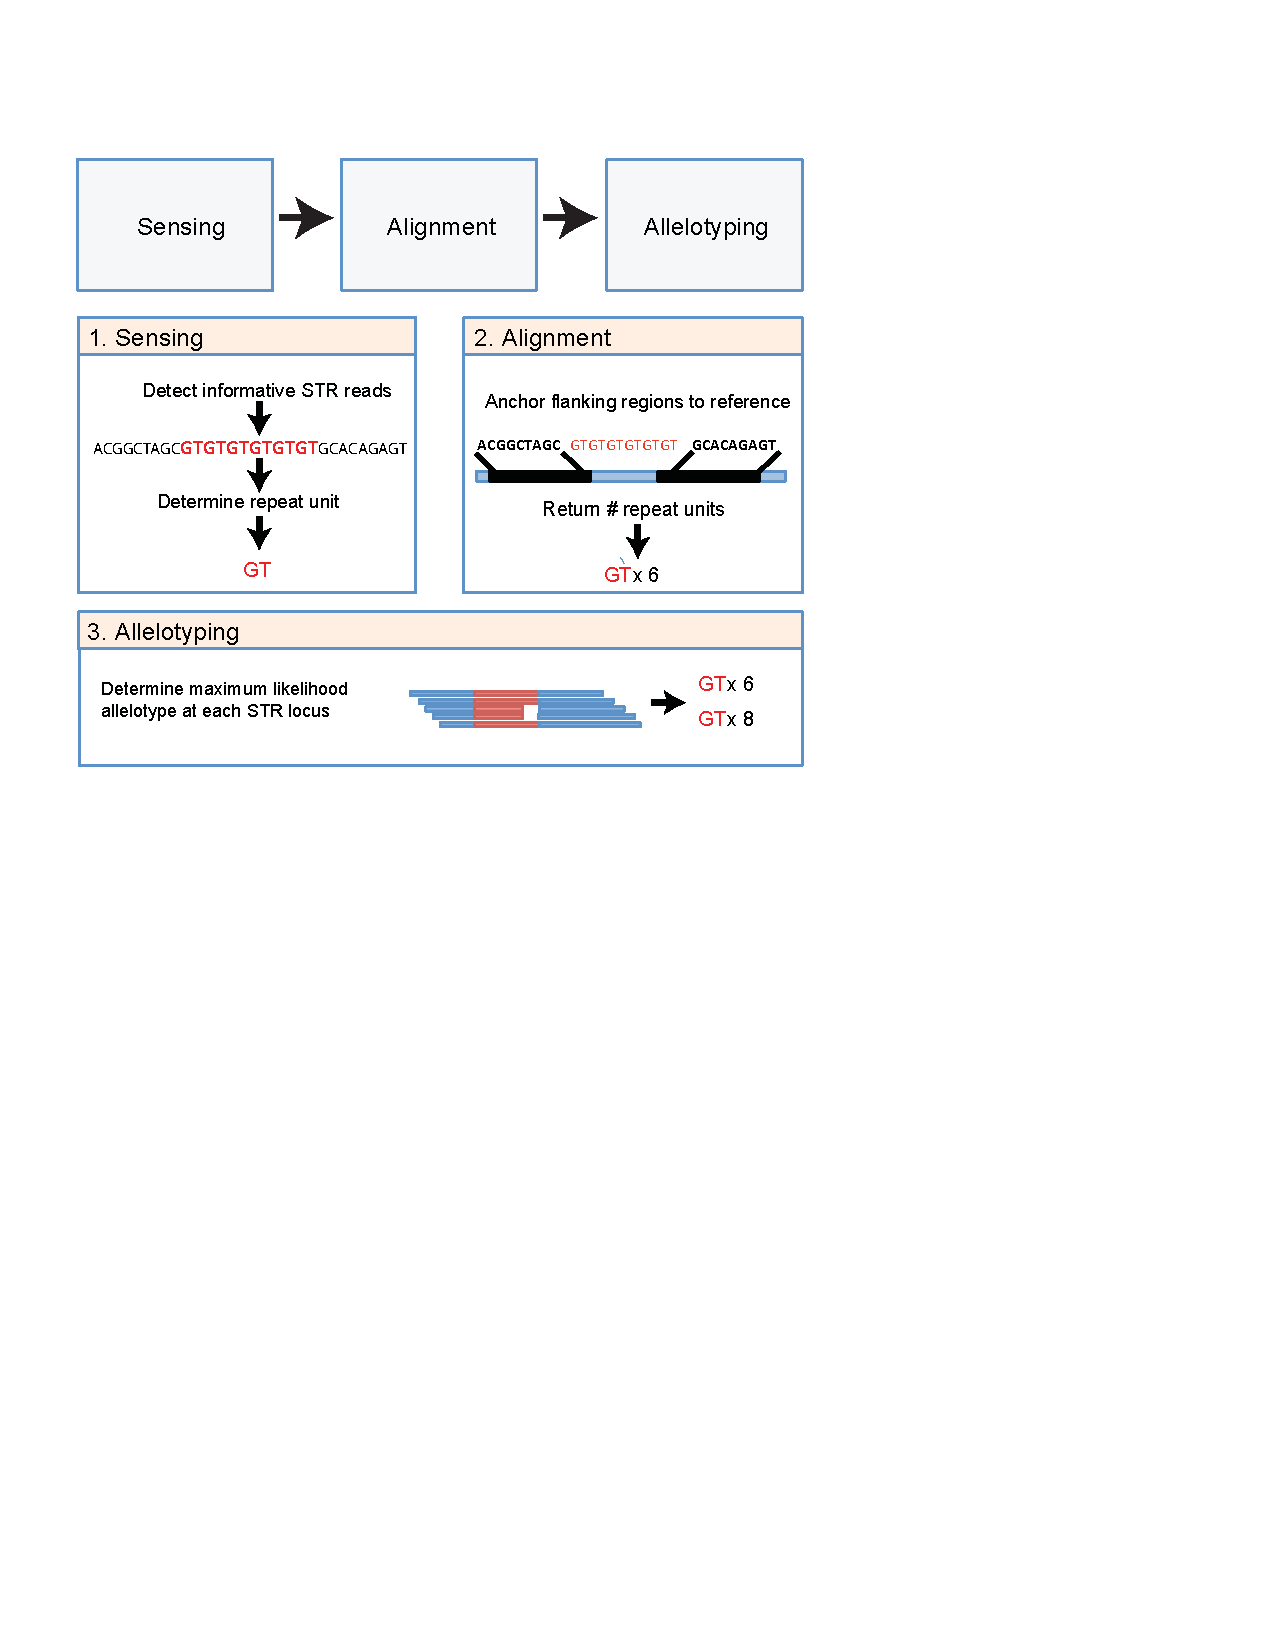
\includegraphics[width=0.5\textwidth]{Figures/Chapter2/Fig1.pdf}
\caption{\textbf{lobSTR algorithm overview} lobSTR consists of three steps. The sensing step detects informative STR reads and determines their repeat motif. The alignment step maps the STRs' flanking regions to the reference. The allelotyping step determines the STR alleles present at each locus.}
\end{figure}

lobSTR implementation offers a complete solution that takes raw sequencing data and reports the alleles present at each profiled STR locus. The program's input is one or more sequencing libraries in FASTA/FASTQ or BAM format. The output is the alignment of STR reads in BAM format and the most likely alleles for each STR locus in a custom tab-delimited text format. lobSTR supports multi-threaded processing.

\section{Results}
\subsection{Comparing lobSTR to mainstream aligners}

We benchmarked lobSTR's alignment performance with reads from an Illumina whole genome sequencing library with 101bp reads (\textbf{Methods \ref{sec:lobmethods}}). To demonstrate its added value for STR profiling over mainstream aligners, we also ran BWA, Novoalign, and Bowtie on the same input data with and without the GATK local indel realignment tool. In addition, we ran BLAT \cite{Kent2002} to characterize STR alignment by a tool that is centered on sensitivity rather than speed. BWA and Novoalign were tested with the default parameters that can detect up to 5bp and 7bp indels, respectively. Bowtie has no indel tolerance and was evaluated as a control condition with tolerance of up to two mismatches. BLAT was tested with the default parameters that can tolerate up to 10\% divergence from the reference, which corresponds to approximately 10bp indels. To focus on the pure algorithm speed-up, all tests were executed on a single CPU.

lobSTR excelled in all the parameters required for efficient STR alignment (\textbf{Table \ref{tab:lobtab1}}). First, lobSTR processed the reads 2.2 times faster than Bowtie, 22 times faster than BWA, 70 times faster than Novoalign, and almost 1000 times faster than BLAT (\textbf{Figure \ref{fig:lobfig2}A}). These results indicate that there is a minimal computational payment in running lobSTR in parallel to mainstream aligners in order to augment variation calling to include STR polymorphisms. Second, as required, lobSTR reported only informative reads that fully encompass STR loci. On the other hand, the mainstream aligners reported between 2,000 to 5,000 non-informative STR reads per million input sequences, which may confound downstream calling algorithms if not removed. Third, lobSTR detected the largest number of informative reads with STR variations compared to mainstream aligners (\textbf{Figure \ref{fig:lobfig2}B}). The other aligners showed a strong tendency to report STR reads with the reference allele vis-a-vis with their indel tolerance. Bowtie did not report any STR variation. After GATK local realignment, BWA and Novoalign, respectively, reported that 20\% and 25\% of the informative reads have STR variations. BLAT reported that 37\% of the informative reads have STR variations, compared to 50\% in lobSTR. Analyzing data collected from a large number of randomly ascertained STR loci \cite{PayseurJingHaasl2011} (Utah Marker Development Group) demonstrates that 33-66\% of STR sequence reads should exhibit a non-reference allele (see Methods). This suggests that lobSTR's results are more representative of the true rate of STR variations than mainstream alignment tools.

\begin{table}
\centering
\label{tab:lobtab1}
\begin{adjustbox}{width=1\textwidth}
\begin{tabular}{l l l l l l l l}
\hline
Algorithm & Indel tolerance (bp) & Time (sec)& \# Non-informative reads & \# Informative reads & \# Var. reads$^a$	& Ratio$^b$ & Peak memory (Gbyte) \\
\hline
lobSTR & - & 109 & 0 & 973 & 485 & 0.5 & 0.3\\
Bowtie&0&258&2,193&523&0&0&2.2\\
BWA&5&2,450&3,026&883&174&0.19&2.5\\
BWA+GATK&5&2,943&2,691&869&172&0.20&2.5\\
Novoalign&7&7,601&4,947&1,024&208&0.2&13.8\\
Novoalign+GATK&7&8,123&4,906&1,047&259&0.25&13.8\\
BLAT&10&108,862&19,919&1,611&602&0.37&3.7\\
\hline
\end{tabular}
\end{adjustbox}
\caption{\textbf{STR Alignment performance across different algorithms.} All results are per million 101bp Illumina reads. $^a$Number of informative reads that show a non-reference allele. $^b$Ratio of reads with the non-reference allele versus total informative STR reads.}
\end{table}

\begin{figure}[h!]
\centering
\label{fig:lobfig2}
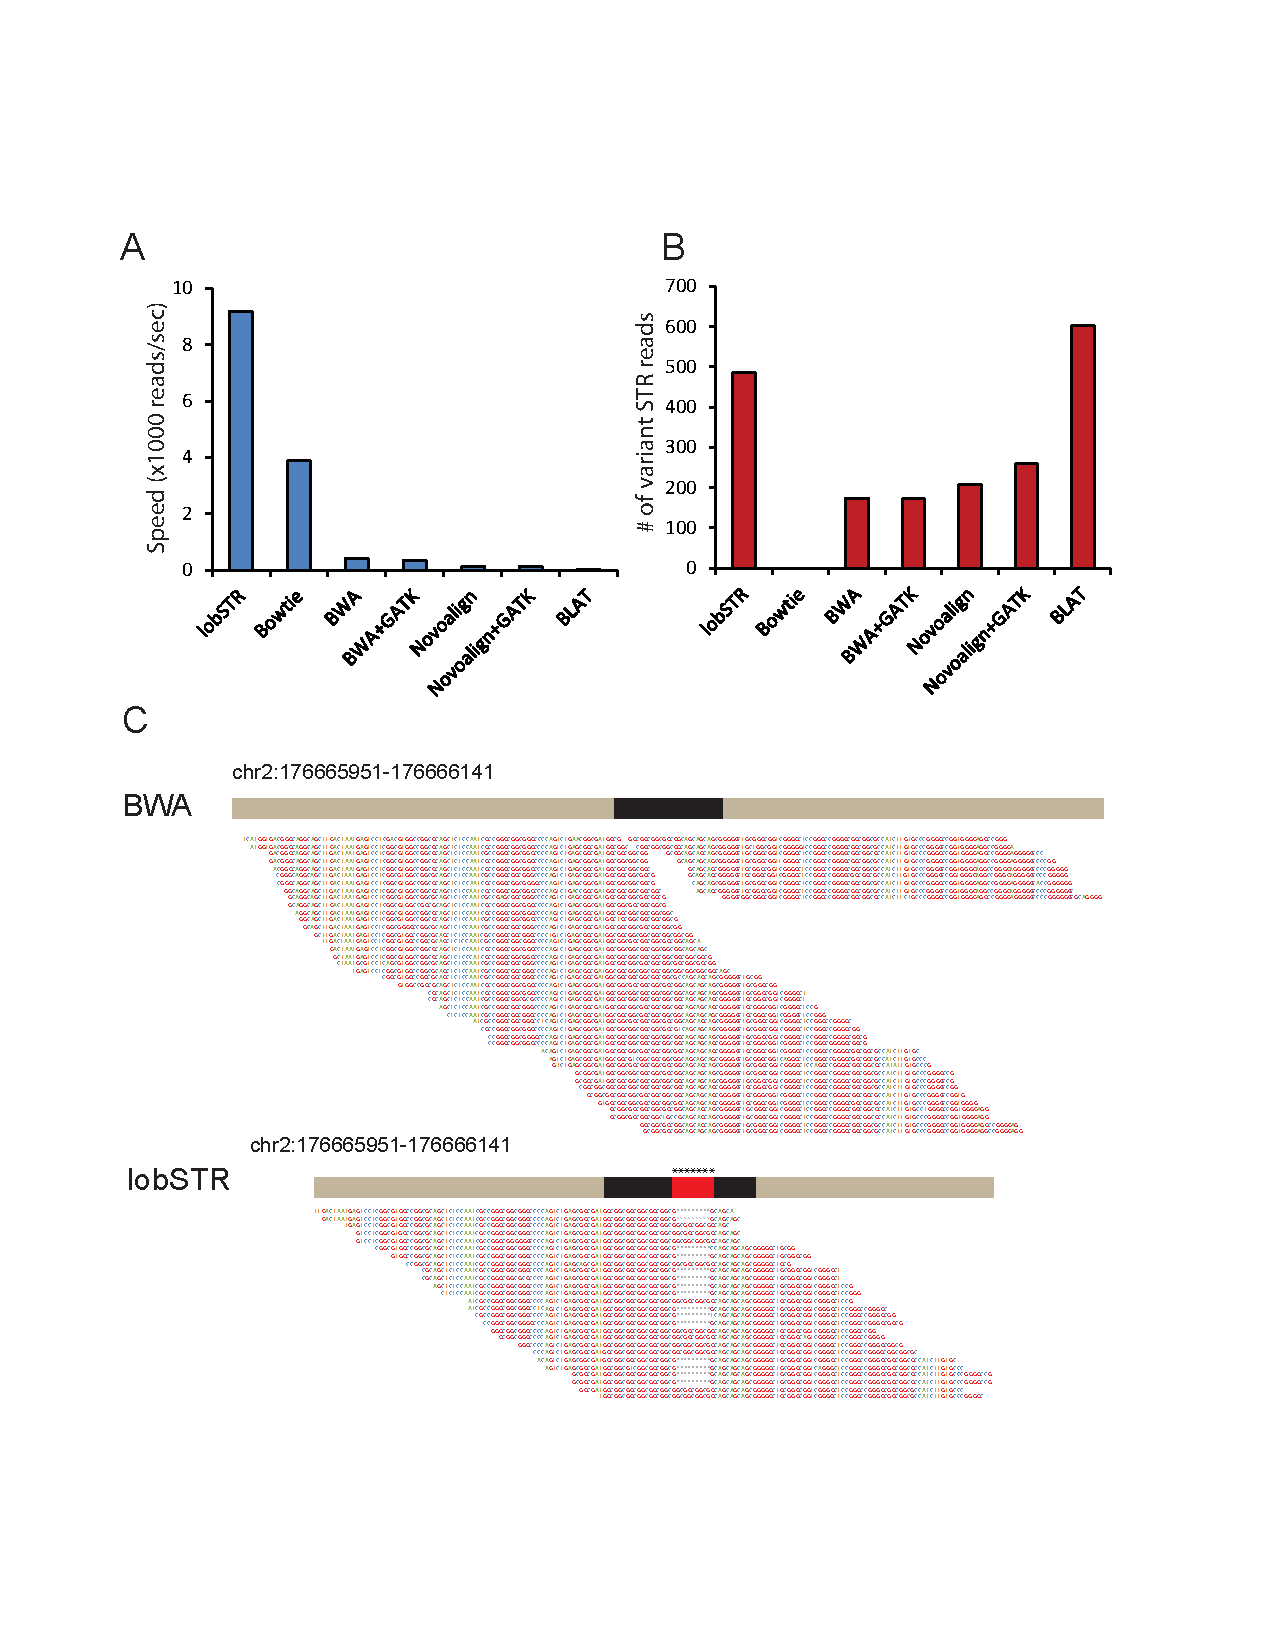
\includegraphics[width=0.5\textwidth]{Figures/Chapter2/Fig2.pdf}
\caption{\textbf{lobSTR shows an added value for STR profiling over mainstream techniques} \textbf{(A) Alignment speed (reads per second) of lobSTR, mainstream alignment and BLAT}. lobSTR processes reads between 2.5 and 1000 times faster than alternative methods \textbf{(B) The sensitivity of detecting STR variations of different alignment strategies.} Only BLAT detected more STR variations than lobSTR \textbf{(C) lobSTR accurately detects pathogenic trinucleotide expansions that are discarded by mainstream aligners.} The figure shows simulation results of the \emph{HOXD13} heterozygous locus with a normal and a pathogenic allele that contains 7 additional alanine insertions. BWA reports only the normal allele. Reads exhibiting a pathogenic STR expansion are not detected. lobSTR identifies both alleles present at the simulated locus. All positions are according to hg18.}
\end{figure}

Reporting STR reads with non-reference alleles is crucial for profiling pathogenic mutations. We further explored whether lobSTR can correctly detect disease alleles of dominant trinucleotide repeat expansion disorders. As test cases, we focused on two conditions that can be theoretically profiled using standard Illumina runs. The first condition was a GCN expansion in \emph{PABPN1} that causes oculopharyngeal muscular dystrophy (OPMD) \cite{BraisBouchardXieEtAl1998}, where the normal allele exhibits 10 repeats and the pathogenic allele spectrum for the dominant form is between 12 to 17 repeats \cite{PearsonNicholEdamuraCleary2005}. The second condition was a GCG expansion in \emph{HOXD13} that is implicated in synpolydactyly \cite{MuragakiMundlosUptonEtAl1996}, a severe limb malformation, where the normal allele is 15 repeats and the documented pathogenic allele spectrum is between 22-29 repeats \cite{PearsonNicholEdamuraCleary2005}. To simulate each condition, we generated 100 reads of length 101bp that were equally sampled from the disease locus consisting of a normal and pathogenic allele with 100bp flanking upstream and downstream regions with 1\% sequencing error rate. For both simulated disease conditions, lobSTR accurately aligned the normal and pathogenic reads to the correct location in the genome. All aligned reads were informative and the allelotyping step correctly assigned a heterozygous state to the disease loci with the correct repeat lengths: (10,15) for \emph{PABPN1} and (15, 22) for \emph{HOXD13}. In stark contrast, BWA failed to correctly align reads from the pathogenic alleles of both loci. Only reference reads were reported (\textbf{Figure \ref{fig:lobfig2}C}).

\subsection{Measuring lobSTR concordance using biological replicates}
To explore the precision of lobSTR, we conducted genome-wide STR profiling of blood and saliva samples from the same individual \cite{LamClarkChenEtAl2012}. These samples were sequenced using Illumina HiSeq2000 with 101bp PE to a mean autosomal coverage of 50x and 102x, respectively. lobSTR ran with default parameters on 20 CPUs and analyzed the two datasets within 12 and 22 hours respectively. After filtering loci with low quality calls, 143,793 shared STRs were covered in the two datasets with at least one read and 79,771 STRs were covered with 10 reads or more (\textbf{Figure \ref{fig:lobfig3}A}). 

We quantified the rate of discordant autosomal calls between the two samples. We focused on two measurements: the genotype discordance rate and the allelic discordance rate \cite{PompanonBoninBellemainEtAl2005}. The former reports as an error any mismatch between corresponding calls, whereas the latter reports only the fraction of discordant alleles in corresponding calls. For example, consider a locus that is called (A,B) in the saliva sample and (A,C) in the blood sample. This locus shows a single genotype discordance, but only 0.5 allelic discordance, since the A allele was correct. 

Both types of error greatly diminished with sufficient coverage (\textbf{Figure \ref{fig:lobfig3}B,C}). At 5x coverage, the genotype discordance rate was 11\% and the allelotype discordance was 5\%; At 21x coverage, the genotype discordance rate was 3\% and the allelotype discordance rate was 2\%. Similar to STR studies with capillary platforms \cite{WeberBroman2001}, most of the errors were generated in dinucleotide STR loci, whereas other types of STRs showed moderate and similar error rates. The dinucleotide error rates presumably stem from two factors: first, these loci usually show the highest heterozygosity rates \cite{ChakrabortyKimmelStiversEtAl1997,BrinkmannKlintscharNeuhuberEtAl1998,PembertonSandefurJakobssonEtAl2009}. Therefore, they require on average more sequence reads to be correctly called. Second, dinucleotide STRs are more prone to stutter noise \cite{Ellegren2004} and their higher error rates might be due to residual noise after lobSTR stutter deconvlution.

\begin{figure}[h!]
\centering
\label{fig:lobfig3}
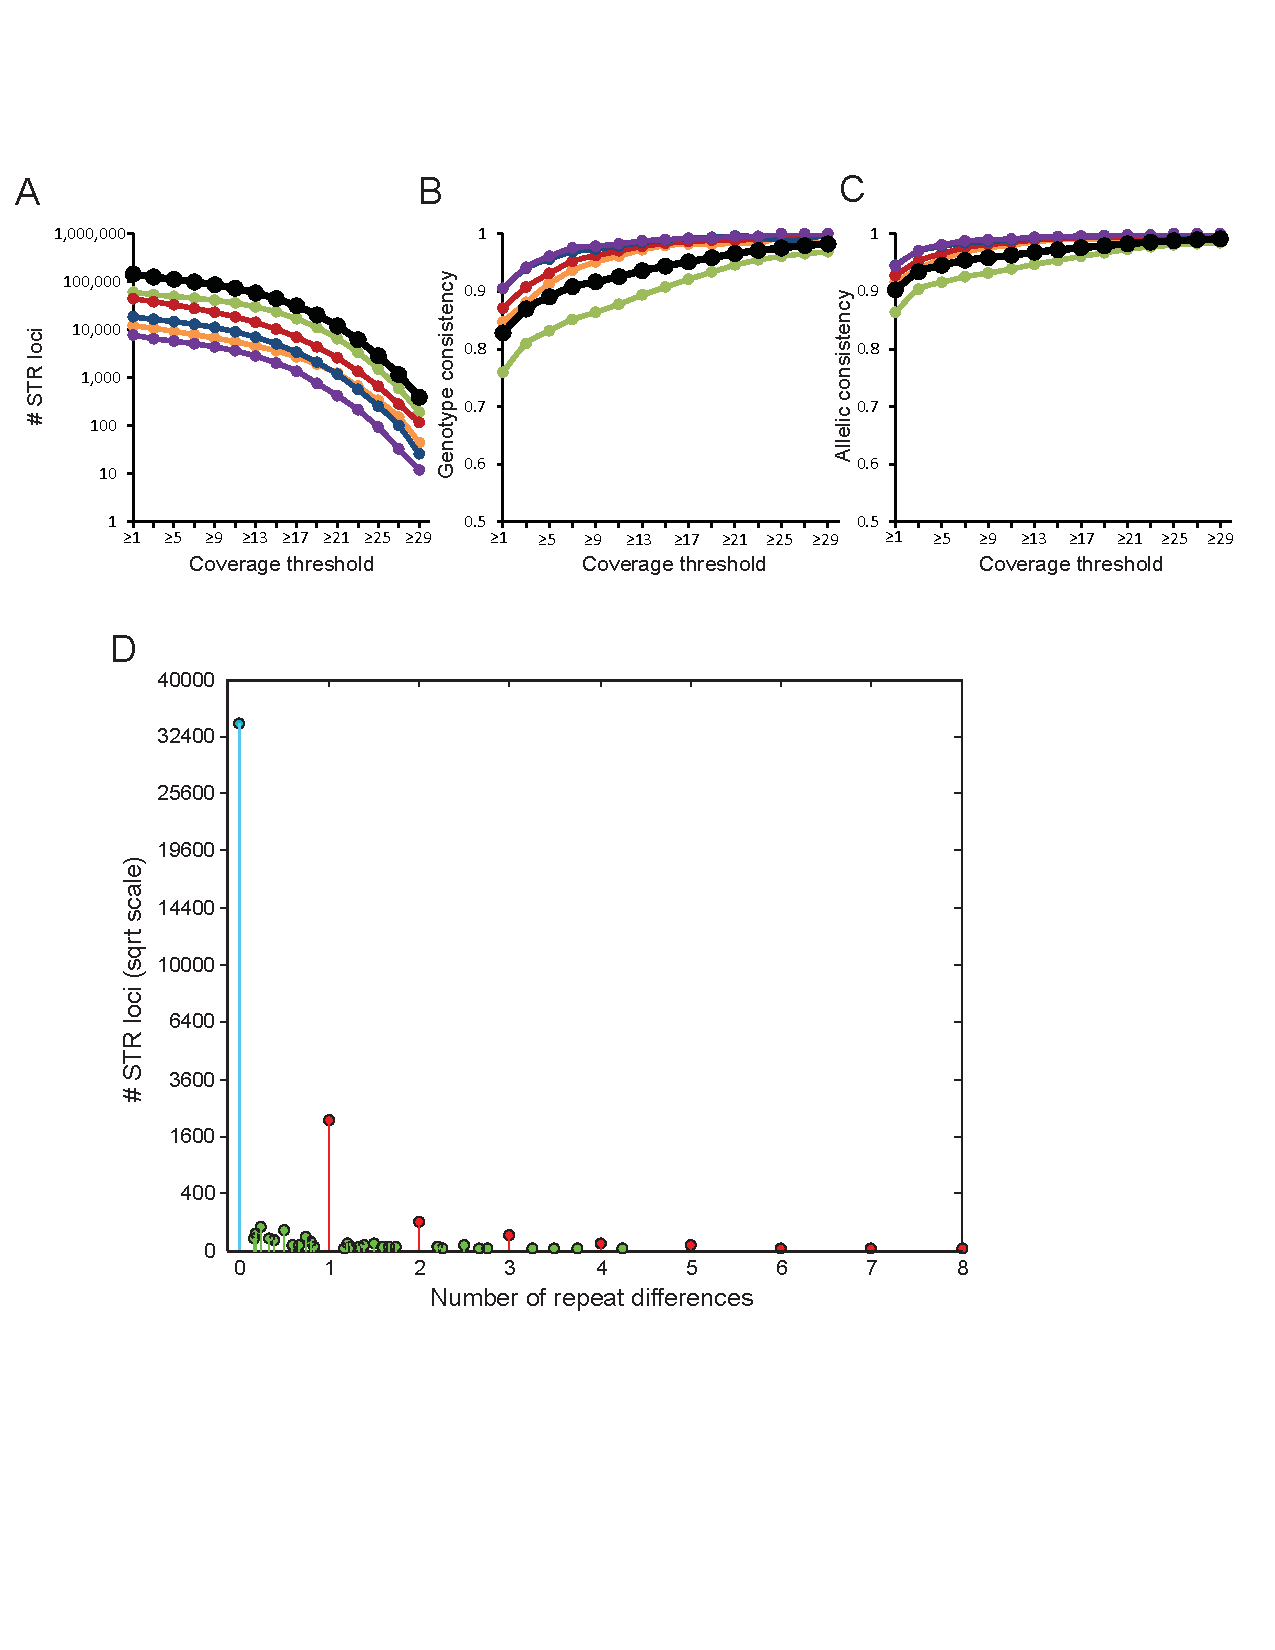
\includegraphics[width=0.5\textwidth]{Figures/Chapter2/Fig3.pdf}
\caption{\textbf{Measuring lobSTR consistency from two samples of the same individual} (A-C) (green - period 2, orange - period 3, red - period 4, blue - period 5, purple - period 6, black - all) \textbf{(A) Loci covered in both samples at increasing coverage thresholds.} \textbf{(B) The genotype discordance rate as a function of coverage threshold.} \textbf{(C) The allelic discordance rate as a function of coverage threshold.} \textbf{(D) Number of repeat differences at heterozygous loci.} Blue - no difference; red - integer numbers of repeat differences; green - non-integer numbers of repeat differences. Most discordance calls consist of a single repeat unit difference between calls in the two samples. Distance was measured as the second minimum distance between alleles of the two samples. The y-axis is given in a square root scale.}
\end{figure}

We further analyzed the STR length differences in discordant calls. To avoid analyzing errors that are simply due to allele drop-outs, we focused on discordant calls that were both heterozygous in blood and saliva. At a coverage of ≥5x, more than 90\% of the errors showed a single repeat unit difference and 99\% of the errors were within two repeat units (\textbf{Figure \ref{fig:lobfig3}D}). This indicates that incorrect alignment of STRs has a minimal effect on allelotyping results, and that stutter is likely the main source of noise. We also found that only 0.8\% of calls at heterozygous loci showed a difference due to an incomplete repeat unit. This highlights that lobSTR can determine STR alleles at a single base-pair resolution. 

\subsection{Tracing Mendelian inheritance using lobSTR}
To further explore lobSTR performance, we conducted a genome-wide STR profiling of a HapMap trio - a father (NA12877), mother (NA12878), and son (NA12882) -- from the CEU population that were sequenced using 100PE reads on a HiSeq2000 (\textbf{Table \ref{tab:lobtab2}}). The average autosomal coverage was 50x and average STR coverage was 14x. At $\geq$10x coverage threshold, 57\% of the STRs in the CEU trio had a non-reference allele. 

\begin{table}
\centering
\label{tab:lobtab2}
\begin{tabular}{l l l l l}
\hline
Individual	& Relationship & Input reads	& STR Aligned reads	& Mean STR Coverage \\
\hline
NA12878 &	Mother	& 1,708,169,546 &	3,398,933 &	14.8 \\
NA12877	& Father &	1,637,816,924	&3,212,073 &	14.1 \\
NA12882	& Son	& 1,625,404,856 &	3,183,795 &	14.0 \\
\hline
\end{tabular}
\caption{\textbf{Profiling STRs in Illumina reads from a HapMap trio.}}
\end{table}

In general, deviations of offspring's STR alleles from Mendelian inheritance (MI) indicate a potential calling error \cite{EwenBahloTreloarEtAl2000}. With 5x coverage across all trio members, the MI rate was 95\%; with 10x coverage, MI was 97\%; and with coverage threshold of 15 or more, MI was 99\%. (\textbf{Figure \ref{fig:lobfig4}A}). We also repeated the analysis only with discordant parental sites (for example, A/B call in one parent and A/C call in another parent). We noticed a drop to 93\% in the MI patterns with a low coverage threshold of 5x, which is mainly because of partial coverage of heterozygous sites in the parents. The MI rate was recovered to the same level with higher coverage threshold. At 17x coverage 99\% of sites showed a perfect Mendelian segregation pattern (\textbf{Figure \ref{fig:lobfig4}B}). 

\begin{figure}[h!]
\centering
\label{fig:lobfig4}
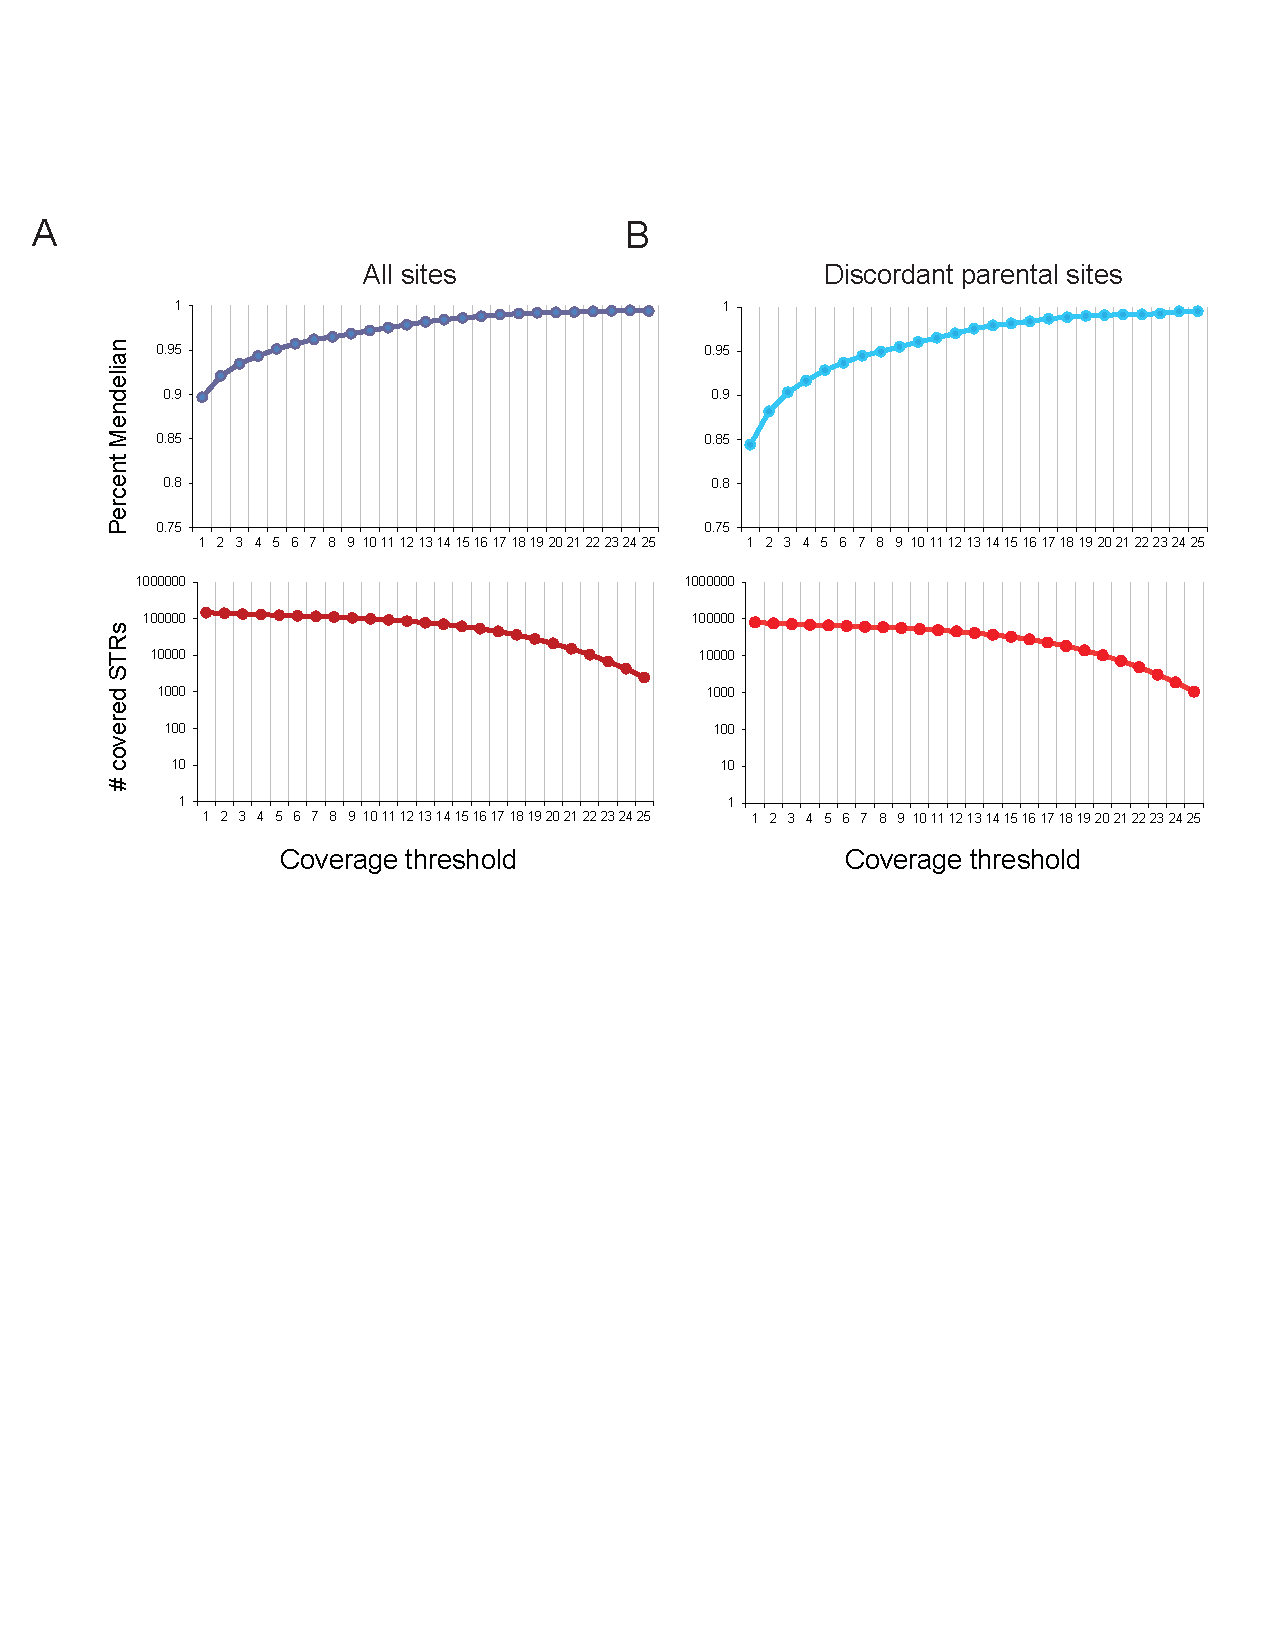
\includegraphics[width=0.5\textwidth]{Figures/Chapter2/Fig4.pdf}
\caption{\textbf{Validating lobSTR by Mendelian inheritance in a HapMap trio.} Mendelian inheritance (blue) rose to 99\% above 17x coverage. The number of covered loci at each coverage threshold is shown in red. \textbf{(A) Mendelian inheritance of all covered loci.} \textbf{(B) Mendelian inheritance of loci with discordant parental allelotypes.}}
\end{figure}

\subsection{Validating lobSTR accuracy with DNA electrophoresis}
We sought to compare lobSTR calls to the results of DNA electrophoresis, which is considered the gold standard for STR allelotyping. First, we focused on a set of STR markers that are used for forensic DNA fingerprinting. As an input for lobSTR, we sequenced a male genome from our lab collection with three runs of Illumina GAIIx for 101PE cycles that yielded ~740 million reads. The autosomal sequencing coverage was 36x according to alignment with mainstream algorithms. lobSTR identified 1.6 million informative reads that mapped to $\sim$140,000 STR loci, with an average of 4.91x coverage of diploid STR loci. In parallel, we used a commercial forensic kit to genotype 14 autosomal STR markers on a capillary electrophoresis platform. Thirteen out of 14 markers were covered by at least a single sequence read and 8 markers were covered by at least 3 sequence reads. The marker that was not covered spanned more than 129bp, exceeding the limit for detecting informative reads with the 101bp sequence reads.

We observed good concordance between lobSTR and the capillary results (\textbf{Table \ref{tab:lobtab3}}). lobSTR correctly called all but one of the 8 markers that were covered by at least 3 reads and most of the alleles in loci that were covered with 2 or less reads. Remarkably, some of these markers, such as D8S1179, displayed two heterozygous alleles that did not match the reference. Other alleles, such as in Penta D and Penta E, correctly returned 20bp and 25bp length differences from the reference allele, respectively. The capillary results of one tetranucleotide marker, THO1, exhibited a non-integer number of copies (9 repeats + 3bp). lobSTR reported exactly the same results, further demonstrating that STRs can be called within a single base pair resolution. lobSTR also correctly called a homozygous STR that was covered by a single read. In another 4 markers with coverage of ≤2x, lobSTR correctly called one allele and missed the other allele due to sequencing coverage. We observed only a single erroneous call due to stutter noise in the D5S818 locus. This homozygous locus was covered by three sequence reads: two correct and one with a single repeat expansion. With such a low sequencing coverage, the allelotyping algorithm was not able to identify the noisy read and assigned a heterozygous state to the locus. 

\begin{table}
\centering
\label{tab:lobtab3}
\begin{adjustbox}{width=1\textwidth}
\begin{tabular}{l l l l l l l l}
\hline
STR locus & lobSTR (bp) & Converted lobSTR & Capillary & Hg18 & Repeat & Coverage & Result$^a$\\
\hline
D8S1179 & -8/8 & 11/15 & 11/15 & 13 & [TCTA]n & 13 & Y\\
CSF1PO & -12/-4 & 10/12 & 10/12 & 13 & [AGAT]n & 13 & Y\\
TPOX & 0/12 & 8/11 & 8/11 & 8 & [AATG]n & 12 & Y \\
THO1 & 11/11 & 9.3/9.3 & 9.3 & 7 & [AATG]n & 11 & Y\\
D16S539 & 4/12 & 12/14 & 12/14 & 11 & [GATA]n & 5 & Y\\
D7S820 & -20/-8 & 8/11 & 8/11 & 13 & [GATA]n & 3 & Y\\
Penta D & -20/0 & 9/13 & 9/13 & 13 & [AAAGA]n & 3 & Y\\
D5S818 & 0/4 & 11/12 & 11 & 11 & [AGAT]n & 3 & E \\
D3S1358 & -4/-4 & 15/15 & 15/17 & 16 & [TCTN]n & 2 & P\\
PentaE & 25/25 & 10/10 & 10/15 & 5 & [AAAGA]n & 1 & P \\
FGA & -4/-4 & 21/21 & 21/24 & 22 & [TTTC]n & 1 & P\\
D18S51 & -12/-12 & 15/15 & 15 & 18 & [AGAA]n & 1 & Y\\
D13S317 & 4/4 & 12/12 & 11/12 & 11 & [TATC]n & 1 & P\\
\hline
\end{tabular}
\end{adjustbox}
\caption{\textbf{Capillary platform results versus lobSTR results for the CODIS set.} $^a$Y - both platforms agree. P - lobSTR reported only one allele out of two. E - lobSTR reported an allele that does not exist.}
\end{table}

Next, we evaluated lobSTR calls made in 12 low-pass sequenced genomes from the Human Genome Diversity Project (HGDP) \cite{GreenKrauseBriggsEtAl2010,ReichGreenKircherEtAl2010}. Five genomes had coverage of 1.4x-1.9x with 109bp reads, and the other seven had coverage of 4.8x-7.7x with 77bp reads (\textbf{Supplemental Table 3}). One hundred and ninety five STRs with equivalent entries in the lobSTR reference have been genotyped in these genomes using DNA electrophoresis as part of the CEPH-HGDP panel \cite{RamachandranDeshpandeRosemanEtAl2005,PembertonSandefurJakobssonEtAl2009}. Combining lobSTR results from all datasets gave 59 comparable markers with coverage of 3-5 reads with a median coverage of 3x (\textbf{Supplemental Table 4}). Despite the low coverage, lobSTR correctly returned 75\% of the genotypes and 85\% of the allele calls. Most of the alleles showed at least 5bp difference from the reference and some alleles showed a difference of 24bp and were correctly called. We did not observe a significant correlation between errors and the size of the variation. 

\subsection{Genome-wide STR profiling confirms previously locus-centric observations}
Encouraged by the accuracy and speed of lobSTR, we harnessed our pipeline to establish a reliable reference for future studies. Our input dataset was a male individual that, as of today, has been sequenced to highest coverage of 126-fold from a blood sample \cite{AjayParkerAbaanEtAl2011}. Fourteen billion sequencing reads were obtained from 100bp PE runs on Illumina GAIIx and HiSeq 2000. lobSTR ran for 26 hours using 25 CPUs. It aligned $\sim$6 million reads to approximately 180,000 STR loci out of the 249,000 in the Tandem Repeat Table reference with average coverage 20.82 for autosomal loci. The average reference allele length of undetected loci was 150bp, whereas the mean reference length of detected loci was 41bp. Therefore, in most cases, the undetected loci could not physically be spanned by a single read of the current sequencing length.

We assigned each autosomal STR to one of four allelotype categories: both alleles match the reference (homozygous reference), one allele matches the reference (heterozygous reference), both alleles do not match the reference but are the same (homozygous non-reference), and both alleles are different and do not match the reference (heterozygous non-reference). In all previous experiments, a coverage threshold of 20x resulted with near-perfect STR calling even for dinucleotide loci. To increase the reliability of our results, we focus the analysis on the 97,844 loci that were called with at least this sequencing coverage. The length distribution of these alleles in the reference was mainly between 25-50bp with a low number of very long STRs (\textbf{Figure \ref{fig:lobfig5}A}). 

Similar to the other genomes in this study, 55\% (52,338) of the STR loci differed from the reference: 22,271 (23\%) loci were heterozygous reference, 15,515 (16\%) loci were homozygous non-reference, and 14,552 (15\%) loci were heterozygous non-reference. The other 43,335 (45\%) loci were homozygous reference. Some of the variations reached to 49bp difference from the reference allele. On average, STR variations showed 6.3bp difference from the reference allele and 41\% of the variations were more than 5bp away from the reference (\textbf{Figure \ref{fig:lobfig5}B}). Thus, mainstream-dependent analysis pipelines that can tolerate only a few nucleotide indels, such as BWA, are likely to miss most STR variations.

The genome-wide STR dynamics reported by lobSTR confirm previous findings of locus-centric studies. The rate of STR polymorphism showed a striking correlation with the repeat unit length (\textbf{Figure \ref{fig:lobfig5}C}). Dinucleotide STRs are nearly equally likely to fall into any of the above four categories, whereas hexanucleotide STRs are most likely to match the reference. This trend matches results of a previous study that measured the mutation rate of a few hundreds of Y-STR loci as a function of repeat unit length \cite{JarveZhivotovskyRootsiEtAl2009}.  Similar to our results, the authors showed that penta- and hexanucleotide repeats mutate at half the rate of tri- and tetra-nucleotide repeats. We also found that the rate of STR polymorphism is significantly correlated to the length of the STR allele in the reference (\textbf{Figure \ref{fig:lobfig5}D}). The non-reference loci (n=52,338) had significantly greater lengths than loci that are homozygous reference (n=43,335) (p<0.05, one-sided Mann-Whitney test for each allelotype category versus reference) as previously reported in studies that analyzed a few dozen STRs \cite{BrinkmannKlintscharNeuhuberEtAl1998,Ellegren2000}. 

\begin{figure}[h!]
\centering
\label{fig:lobfig5}
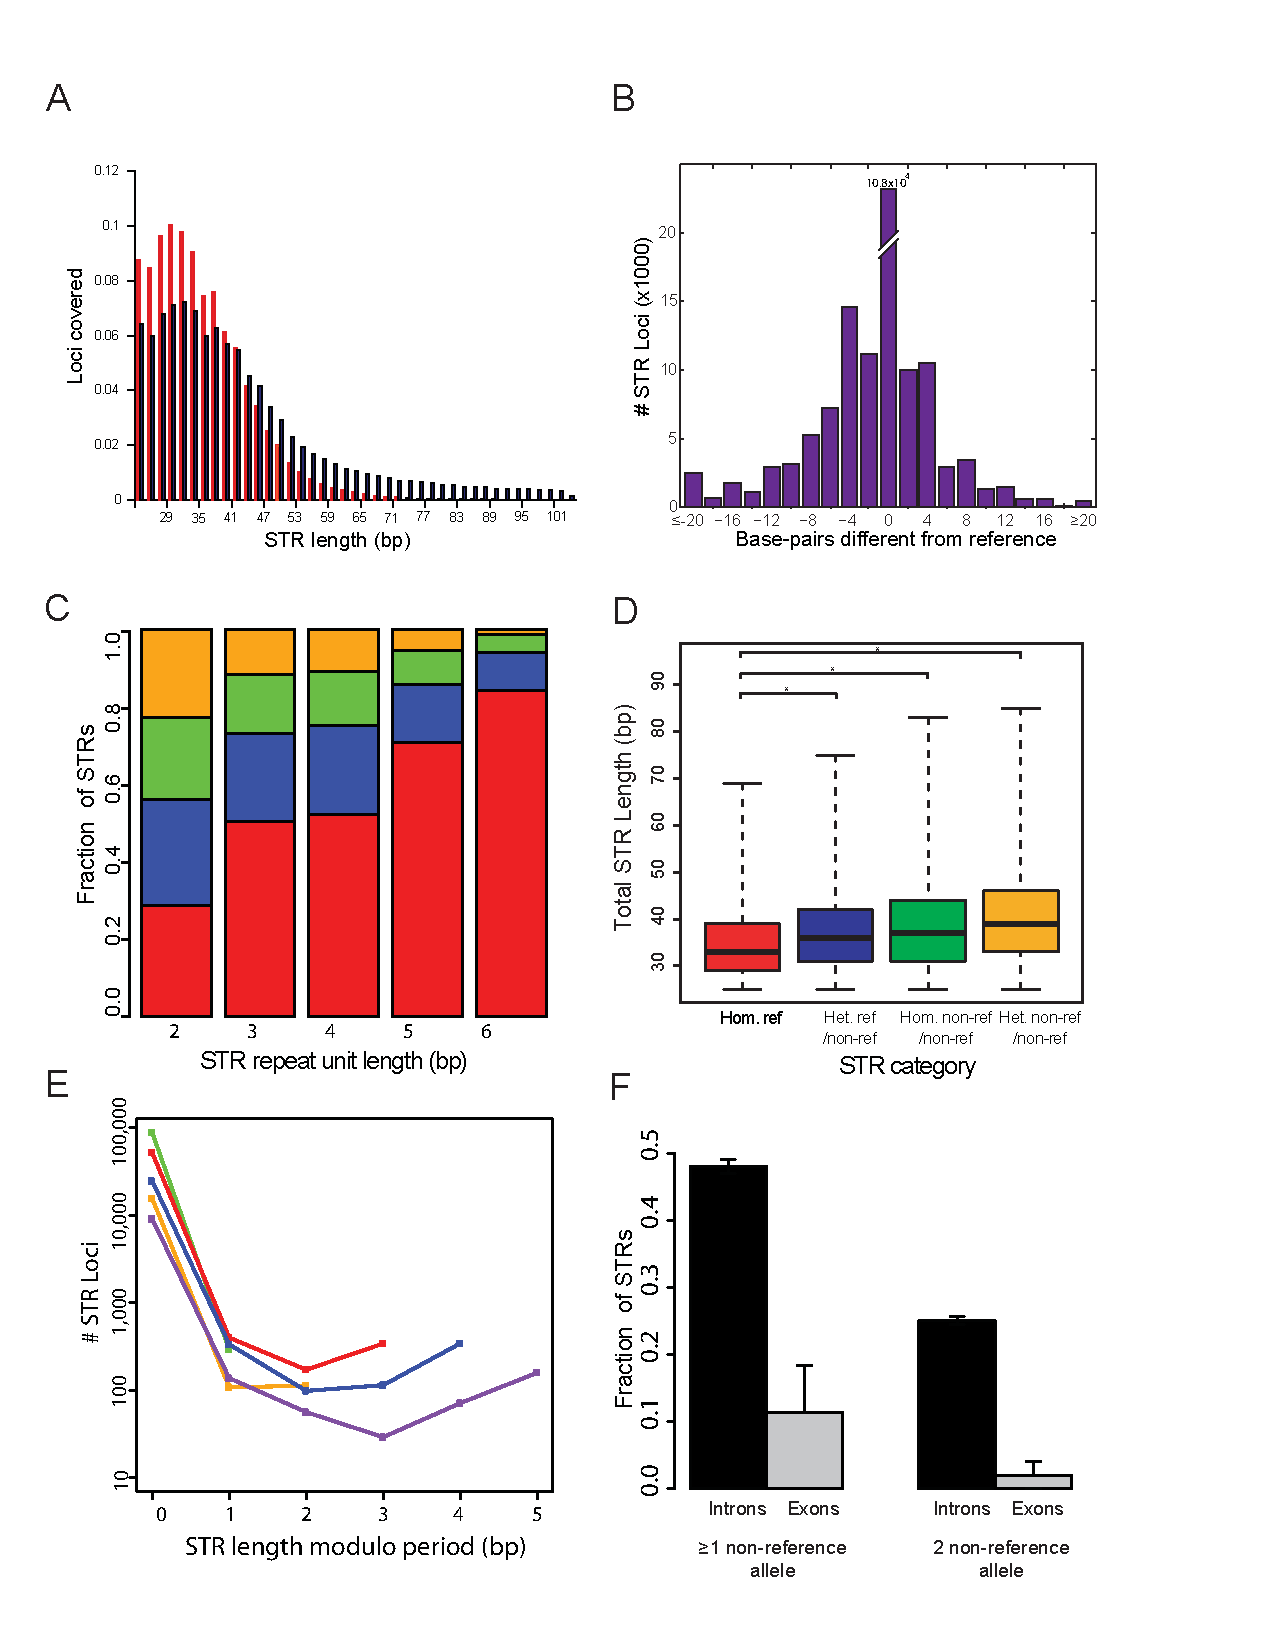
\includegraphics[width=0.5\textwidth]{Figures/Chapter2/Fig5.pdf}
\caption{\textbf{Genome-wide STR profile of an individual.} \textbf{(A) Distribution of STRs with 20x coverage or more as a function of the allele size in hg18.} \textbf{(B) Distribution of allele size differences from reference in lobSTR calls.} The average difference was 6.3bp away from the reference. \textbf{(C) STR polymorphism as function of period.} The number of STR alleles matching the reference sequence increases with increasing repeat unit length (the colors in the entire panel are as follows: red - homozygous reference, blue - heterozygous non-reference/reference, green - homozygous non-reference/non-reference, orange - heterozygous non-reference/non-reference \textbf{(D) Longer STR regions are more polymorphic.} The median STR length (thick black line) increases with the number of variant alleles. * denotes a significant (p<0.05) difference according to a one-sided Mann–Whitney test. Boxes denote the interquartile range and whiskers denote 3 times the interquartile range. \textbf{(E) lobSTR shows mutational trends at single base pair resolution.} The number of base pairs difference from reference modulo the period size versus the number of alleles detected (in logarithmic scale) is shown for each period (green - period 2, orange - period 3, red - period 4, blue - period 5, purple - period 6). Incomplete STR unit differences tend to differ by a full unit +/- 1bp from the reference. \textbf{(F) Fraction of trinucleotide STRs with non-reference alleles in introns versus exons.} 95\% confidence intervals are given by the error bars.}
\end{figure}

We also used lobSTR to determine genome-wide trends of STRs at single base pair resolution (\textbf{Figure \ref{fig:lobfig5}E}). Overall, 99\% of alleles varying from the reference allele showed differences that were complete multiples of the STR unit. This trend varied by period, with dinucleotide STRs least likely (0.3\%) to differ by an incomplete motif unit and hexanucleotide most likely (4.7\%).

Finally, lobSTR reported significant differences between repeat variations in intronic and exonic regions (\textbf{Figure \ref{fig:lobfig5}F}). Intronic trinucleotide STRs were twice as likely to exhibit at least one non-reference allele than exonic regions (0.480-0.502 95\% CI and 0.179-0.336 95\% CI for introns and exons, respectively), and nearly five times as likely to exhibit two non-reference alleles (0.107-0.119 95\% CI and 0-0.047 95\% CI for introns and exons, respectively). Significantly, lobSTR reported that 1.9\% (62 out of 3276) of the intronic trinucleotide STRs showed length differences that were not a multiple of three nucleotides. On the other hand, all reported exonic trinucleotide variants retained the reading frame. In addition, lobSTR allelotyped 34,667 intronic and 7 exonic non-trinucleotide STRs. Of the intronic non-trinucleotide STRs, 18,277 (53\%) showed at least one allele with a frameshift deviation, and 8,686 (25\%) showed two frameshifted alleles. Surprisingly, 3 of the 7 exonic loci, all tetranucleotides, showed expansions by units of 4bp, which would result in a frameshift mutation. In one case, in exon 8 of DCHS2, the frameshift variation was homozygous. This call was supported by 33 independent reads, showing a potential loss of function in this gene.

Taken together, the overall findings of lobSTR in this genome serve as a biological validation for the accuracy and utility of genome-wide STR profiling using our technique.

\section{Discussion}
STR profiling techniques have changed very little in the past two decades, relying on the faithful yet cumbersome capillary electrophoresis technique to scan a few dozen loci at a time. The advent of HTS has ushered in the opportunity to conduct genome-wide STR variation analyses. Here, we presented an end-to-end solution for this task. Our solution bypasses the gapped alignment problem, has no inherent indel limitation, and can reliably profile highly polymorphic STRs at a single base pair resolution. We provided a detailed comparison between lobSTR and popular mainstream aligners and showed that even with long reads, these aligners are significantly biased towards the detection of the reference allele. We have established the feasibility of lobSTR to profile STR loci from a total of 20 genomic datasets and demonstrated the strategy's accuracy by analyzing its consistency, ability to trace Mendelian inheritance, and comparing its results to orthogonal molecular techniques. Moreover, our genome-wide STR analysis confirms previous biological observations, which further highlights the algorithmic validity. 

lobSTR results from the trio genomes and the Ajay et al. genome consistently showed genome-wide polymorphism rates of 55\%-57\% for STRs with lengths 25bp and over. A recent study by McIver et al. \cite{McIverFondonSkinnerEtAl2011} evaluated the performance of STR calling using post-BWA alignment files with a set of quality rules. Using a mixture of Illumina 45-100bp reads and 454 reads from two trios in the 1000Genoems project, they reported that 1.1\% of the STRs with lengths of 20bp and over were polymorphic. We wondered if the polymorphism discrepancy between the studies could be explained by the shorter reading lengths in the McIver study that biased their calls to very short, less polymorphic STRs. However, when we ran lobSTR on the 1000Genomes CEU trio datasets (Methods), we found again that 57\% of the STRs were polymorphic (25,885 out of 45,461 STRs that were called with ≥5x coverage at the three genomes). These results suggest that STR profiling that is restricted by the default BWA indel tolerance -- 5bp for the Illumina datasets in the McIver et al. study -- can significantly reduce the sensitivity for observing STR variations. 

We envision that lobSTR will be used in parallel to conventional analysis pipelines in order to augment variation calling to STR loci. The fast running time of our algorithm should not impose a significant computational burden on users. A low coverage genome of 5x takes about an hour on a standard server with 25 CPUs, a high coverage genome of 30x takes eight hours using the same settings, and a ultra-high covered genome of 126x takes 26 hours (\textbf{Supplemental Table 2}).

Currently, the major barrier for STR profiling is the sequencing read length, as the number of detectable STRs is limited to those that are entirely spanned by a single read. To test the effect of genomic coverage on STR profiling, we sampled reads from the 126x genome and calculated the amount of reported STRs (\textbf{Supplemental Figure \ref{fig:lobsup6}}). With genome-wide coverage of 40x, there are more than 100,000 STRs that will be pass an STR-coverage threshold of 10x. However, higher genomic coverage does not linearly improve the number of STRs that pass this threshold, marking a potential upper bound of sequencing read lengths of 100bp. We also explored the utility of the longer reads by Sanger, 454, and IonTorrent for STR profiling of personal genomes using lobSTR (\textbf{Supplemental Table 5} and \textbf{Supplemental Text \ref{sec:lobsupptext}}). Longer reads indeed increased the number of reported STR loci compared to the same autosomal coverage by Illumina. However, out of these, Sanger seemed to be the only method to produce reliable STR reads. We expect that as sequencing reads continue to increase in both length and quality, lobSTR's performance will further improve and allow inclusion of a larger number of STR variations. Ultimately, these will include large pathogenic expansion, such as those in Huntington's disease, which can span more than 100bp. 

As of today, sequence analysis algorithms can detect almost any type of genetic variations, from SNPs \cite{GoyaSunMorinEtAl2010} and indels \cite{KoboldtChenWylieEtAl2009,GoyaSunMorinEtAl2010} to CNVs and chromosomal translocations \cite{ChenWallisMcLellanEtAl2009}. lobSTR adds a new layer of information with tens of thousands of highly polymorphic genetic variations that have a multitude of applications, from personal genomics, to population studies, forensics analysis, and cancer genome profiling.

\section{Methods}
\label{sec:lobmethods}
\subsection{Comparing lobSTR to mainstream aligners}
All alignment strategies were tested in a Linux environment, on a server with 4 twelve-core AMD Opteron 6100 and 128Gbyte of RAM. The following software versions were tested: BWA version 0.5.7, Bowtie version 0.12.7, and Novoalign freeware version 2.7.13, BLAT version 34, and GATK version 1.3-21.

The input was 5 million Illumina reads of the male sample from our lab collection. BLAT results were filtered to include only the top hit for each read. We suppressed multi-mappers in all other tools. Informative STR reads were identified by the intersectBed tool of the Bedtools packages \cite{QuinlanHall2010}. We converted CIGAR scores to the number of base pairs difference from the reference allele by counting any insertions or deletions falling within and directly adjacent to the STR region. Simulating reads from pathogenic STR loci was conducted using a simple Python script available by request from the authors. 

\subsection{Determining the expected number of non-reference reads}

A previous study by The Utah Marker Development Group has shown that 70\% of thousands of randomly chosen tetranucleotide STR loci are polymorphic. We also re-analyzed Payseur et al. data to infer the polymorphism rate in STRs with length ≥25bp in the assembled genome of Craig Venter using results reported in their Supplementary Tables 1-5. Concordant with the Utah study, this rate was 66\%.

The rate of non-reference STR reads is bounded between two extreme cases. The lower bound is that all polymorphic STRs are heterozygous with a reference allele. Thus, only half of the reads from variable loci will show a non-reference allele, which gives 33\% as a lower bound. The upper bound is that all polymorphic STRs are different from the reference in their two alleles. In this case, every read from a variable locus will show a non-reference allele, which gives 66\% as an upper bound.  

\subsection{Biological replicates analysis}
Raw reads for blood-derived and saliva-derived genomic DNA from the same individual were downloaded from the NCBI short read archive (\url{www.ncbi.nlm.nih.gov/sra}) with accessions SRX097307 and SRX097312, respectively. Loci in which (1) less than 75\% of reads agreed with the allelotype call in both samples or (2) the locus was covered in either sample by more than three times the mean coverage level were removed from the analysis.

\subsection{CEU trio data for Mendelian inheritance}
The HapMap CEU trio were NA12877 (father), NA12878 (mother), and NA12882 (son). Raw reads were downloaded from the European short read archive (\url{www.ebi.ac.uk/ena/}) with accessions ERP001228, ERP001229, and ERP001230, respectively. To determine if an STR followed Mendelian inheritance, we required that the alleles detected in the son could be explained by inheriting one allele from each parent. Low quality loci were filtered as described in Biological replicates analysis.

\subsection{Validating lobSTR accuracy using capillary electrophoresis}
Four Catch-All buccal swabs (Epicenter, QEC89100) were used to collect the DNA sample according to the manufacturer protocol. gDNA was extracted by QuickExtract (Epicentre), followed by phenol-chloroform purification and ethanol precipitation. Library preparation was performed according to the standard Illumina protocol. Three runs of 101bp paired-end with a GAIIx platform were used for sequencing. The study was approved by MIT's Committee on the Use of Humans as Experimental Subjects (COUHES). The general sequencing coverage was analyzed as previously reported \cite{ErlichEdvardsonHodgesEtAl2011}. 

Capillary electrophoresis results were obtained from Sorenson Genomics laboratory using the commercial Promega PowerPlex 16 system. To find the genomic positions of these loci, we downloaded corresponding primers that target these loci from the Short Tandem Repeats Internet Database (STRBASE) website (\url{http://www.cstl.nist.gov/strbase/}) of the US National Institute of Standards and Technology (NIST) and used the In Silico PCR tool on the UCSC genome browser to reveal their location. Two loci had proprietary primers and their genomic location could not be identified. The STR repeats in the sequencing file were converted to the PowerPlex allele nomenclature using the NIST definitions.

\subsection{Obtaining CEPH-HGDP STR allelotypes}
STR allelotypes along with a table of RefSeq reference alleles were downloaded from the Rosenberg lab site (\url{www.stanford.edu/group/rosenberglab/repeatsDownload.html}). The allelotypes were given as the number of repeats converted from PCR product size as described in Pemberton et al. \cite{PembertonSandefurJakobssonEtAl2009}. The repeat number is given as reference repeat number plus the difference in product size from the reference divided by the motif size. Sequence data were downloaded from the NCBI Short Read Archive with accessions: ERX004003, ERX004002, ERX004001, ERX004000, ERX0039999, ERX004007, ERX007978, ERX007977, ERX007976, ERX007975, ERX007974, ERX007973, ERX007972.

Using the STS marker table available from the UCSC Genome Browser, we converted the Pemberton et al. markers to hg18 genomic coordinates and annotated them using the TRF table. lobSTR calls that are supported by three or more reads were converted to the Pemberton results. Non-integer repeats reported by lobSTR were rounded to the smallest integer for compatibility with Pemberton data. Markers that could not be faithfully annotated were removed from the analysis.

\subsection{Genome-wide STR profiling of a deeply sequenced personal genome}
Raw sequencing reads for accession number ERP000765 were downloaded from the European Nucleotide Archive's Sequence Read Archive (\url{http://www.ebi.ac.uk/ena/}). The Mann-Whitney test was performed using the wilcox.test function in R. Confidence intervals were calculated using a normal approximation to the Poisson distribution, with a 95\% confidence interval of $\lambda\pm 1.96\sqrt{\lambda}$, where $\lambda$ is the estimated mean of the distribution. Only loci with greater than 20-fold coverage were included in the analysis. Exon and intron coordinates were obtained from the UCSC table browser for human genome build hg18. 

\subsection{1000 Genomes data analysis for the McIver Study}
The HapMap CEU trio were NA12878 (daughter), NA12891 (father), and NA12892 (mother). Raw sequencing reads for the CEU HapMap trios with length of at least 47bp were downloaded from the 1000 genomes NCBI ftp site (\url{ftp://ftp-trace.ncbi.nih.gov/1000genomes/ftp/}). 228, 274, and 214 files were included for individuals NA12878, NA12891, and NA12892. To accommodate the shorter read lengths, lobSTR was run with non-default parameters –fft-window-size 20 –fft-window-step 10, --maxflank 100, and –extend-flank 5. 

\section{Acknowledgements}
Y.E is an Andria and Paul Heafy Family Fellow. This publication was supported by the National Defense Science and Engineering Graduate Fellowship (M.G.) and by a fellowship from the Edmond J. Safra Bioinformatics program at Tel-Aviv University (D.G.). D.G. and S.R. acknowledge support from Israeli Science Foundation grant ISF 1227/09 and an IBM Open Collaborative Research grant. We thank Mona Sheikh, Dina Esposito, and Alon Goren for useful comments on the manuscript, Assaf Gordon for his assistance with multithreading programming, Cole Trapnell for his assistance with preparing lobSTR executables, Mona Sheikh and Sam Sinai for testing lobSTR code, and Dina Esposito for preparing samples for genotyping. 

\section{Supplemental Text}
\label{sec:lobsupptext}
\subsection{lobSTR algorithm}

\subsubsection{Sensing}
The aim of the sensing step is to find informative reads and characterize their STR sequence. The first task of the algorithm is to detect whether a read contains a repetitive sequence. The algorithm breaks the sequence read into overlapping windows with length of $w$ nucleotides and $r$ nucleotide overlap between consecutive windows. In practice, we use $w=24$ and $r=12$. Then, it measures the sequence entropy of each window, according to:

\begin{equation}
E(S_j) = -\sum_{i \in \Sigma}f_i \log_2 f_i
\end{equation}

where $E$ is the entropy, $S_j$ is the sequence of the $j$-th window, $\Sigma$ is the alphabet set, $i$ is a symbol in the alphabet, and $f_i$ is the frequency of symbol $i$. A fully random sequence results in the maximal entropy score that equals to $\log_2(|\Sigma|)$, whereas a repetitive sequence overuses a few symbols and results in a low entropy score, ideally zero in the case of a perfect homopolymer run.

The entropy score proved extremely powerful in discriminating STR sequences from other genomic sequences (\textbf{Supplemental Figure \ref{fig:lobsup2}A}). We calculated the entropy score of sliding windows of 24bp from all documented human STR sequences of repeat unit length of 2-6bp that span up to 100bp. In parallel we scored one million randomly sampled human genomic sequences of 24bp. Then, we classified the input sequences according to their entropy score. The area under the receiver-operating curve (ROC) was 98.3\% when the entropy measurement used the four nucleotides as the input alphabet. We further boosted the classification performance by calculating the entropy using dinucleotide symbols, meaning that “AA” maps to one symbol, “AC” maps to a different symbol, and so forth. In this case, the area under the ROC climbed to 99.4\%, which renders it a nearly perfect classifier. Accordingly, lobSTR uses the dinucleotide symbols for the entropy measure, and we empirically found that an entropy threshold of 2.2 bits provides the optimal performance in terms of speed and number of aligned STR reads.

lobSTR uses the pattern of entropy scores to identify informative reads that fully encompass STR regions. These reads display a series of windows with entropy score below-threshold (the STR region) that are flanked by one or more windows with entropy score above-threshold (the non-repetitive regions) (\textbf{Supplemental Figure \ref{fig:lobsup2}B}). The algorithm only retains reads that follow this pattern. Approximately 97\% of whole genome sequence reads are excluded by this rapid procedure. This significantly contributes to the algorithm's speed, since only a few simple entropy calculations are required to identify the informative STR reads in massive sequencing datasets.

The next task of the sensing step is to determine the length of the repeat unit. Most STR loci do not contain a perfect series of the same repeat unit \cite{Benson1999}. We took a spectral analysis approach that quickly integrates information over the entire STR region to reliably identify the repeat consensus even in imperfect repeats \cite{SharmaIssacRaghavaEtAl2004}. Starting from the window with the lowest entropy score, consecutive windows scoring below the threshold are merged. The sequence of the merged repetitive region is represented as $M$, an $n \times 4$ binary matrix, where $n$ is the number of nucleotides in the repetitive region, the $i$-th row of the matrix corresponds to the $i$-th position of the sequence, and each column corresponds to a different nucleotide type (A,C,G,T). For instance, the DNA sequence ACCGT is represented as:

\begin{equation}
\left[
\begin{array}{c c c c}
1 & 0 & 0 & 0 \\
0 & 1 & 0 & 0 \\
0 & 1 & 0 & 0 \\
0 & 0 & 1 & 0 \\
0 & 0 & 0 & 1 \\
\end{array}
\right]
\end{equation}

The power spectrum of the STR matrix is calculated by performing a Fast Fourier Transform along the columns of the matrix:

\begin{equation}
S(f) = \sum_{y=1}^4 \left( \sum_{x=1}^n M_{x,y} \cdot e^{-\frac{2\pi ixf}{n}} \right) ^2
\end{equation}

Where $M_{x,y}$ is the element in the $x$-th row and $y$-th column of $M$.

STRs have a unique fingerprint in the frequency domain \cite{SharmaIssacRaghavaEtAl2004,ZhouDuYan2009}. Similar to repetitive signals in the time domain, the spectral response of STR elements is characterized by harmonics - a strong signal in recurrent frequency bins and a weak signal in other bins (\textbf{Supplemental Figure \ref{fig:lobsup2}C}). The peaks of the harmonics for a repeat unit of length $k$ dwell in the $\frac{ni}{k} \text{ mod } n$ bins, $i = \{ 0, \pm 1, \pm 2, \hdots \}$. For instance, in a case of n=24, a dinucleotide STR generates a strong signal in bins 0 and $\pm$12. A trinucleotide STR generates a strong signal in bins 0, $\pm$8, and $\pm$16. The algorithm integrates over the normalized energy of the first harmony (i.e. $i$=1) of each possible repeat unit between 2 to 6bp. The consensus repeat unit length is selected according to the highest energy of the corresponding frequency bin (\textbf{Supplemental Figure \ref{fig:lobsup2}D}). Some STR regions may show strong signals in more than one energy bin (i.e., repeats of period 4 show strong energy in both the second and fourth harmonics, and repeats with several insertions or deletions may have more than one strong harmonic). If the second highest harmonic has energy within 30\% of the highest, lobSTR will attempt alignment using the second best period choice if alignment using the first choice fails.

Finally, the algorithm determines the actual STR sequence. It uses a rolling hash function to record all possible $k$-mers in the STR region, where $k$ is the reported repeat unit length described above. The most frequently occurring $k$-mer is set to be the repeat unit of the STR. The output of the sensing step is (a) the consensus sequence of the STR's repeat unit in the canonical form (see Supplemental Methods for the canonical form definition) (b) the sequence read divided into three regions: the STR region, and upstream and downstream flanking regions that correspond to the location of the above threshold windows. 

\subsubsection{Alignment}
The aim of the alignment step is to reveal the identity and the repeat length of an STR-containing read. We do not attempt to align the entire sequence read to the genome to avoid time-prohibitive gapped alignment. Instead, lobSTR employs a divide-and-conquer approach. It separately anchors the upstream and downstream flanking regions of STR-containing sequence reads, without mapping the STR region itself. This procedure identifies the genomic location of the STR and reveals the repeat length by measuring the distance between the flanking regions.

A major challenge of the divide-and-conquer approach is to specifically map the short flanking regions to the genome. To circumvent this problem, we restrict the alignment to STR loci with the same repeat sequence that was reported by the sensing step. We built a reference that holds the flanking regions of all the 240,351 STR loci with repeat unit 2-6bp in the human genome according to the Tandem Repeat Finder table \cite{Benson1999}. The flanking strings are compressed using a Burrows Wheeler Transform \cite{BurrowsWheeler1994} (BWT) to allow efficient searching. All flanking strings of STRs with the same repeat structure are organized under the same BWT structure (Supplemental Methods). Thus, lobSTR only searches a single BWT data structure that corresponds to the repeat sequence, which typically holds up to a few thousand loci. Then, lobSTR intersects the potential mapping positions of the upstream and downstream regions to identify a single compatible location and excludes multiple mappers. This procedure not only speeds up the alignment, but enables higher rates of unique mapping even when the flanking regions are only a few nucleotides long. 

To determine the length of the STR in the read, the algorithm uses the following equation: 

\begin{equation} \label{eq:alnstep}
L = s - (d - u ) + L_{ref}                                                                  
\end{equation}

Where $L$ is the observed STR length, $s$ is the length of the sequence read, $d$ is the genomic coordinate of the last nucleotide in the downstream region, $u$ is the genomic coordinate of the first nucleotide of the upstream region, and $L_{ref}$ is the length of the STR region in the reference genome. 

One important aspect of Eq. 4 is that inaccuracies in the sensing step regarding the exact boundaries of the STR do not affect the reported length of the STR. However, insertions or deletions in the flanking regions might be reported as STR differences, although they are not actual differences in the STR region itself. To mitigate this issue, lobSTR performs local realignment of the entire read once a match is found using the \cite{NeedlemanWunsch1970}. Indels that are detected in the flanking regions are not taken into account and removed from Eq. \ref{eq:alnstep}, providing accurate length calling of the STR region. In addition, the local realignment is used to produce a CIGAR string with the locations of the indels in the read. Downstream genotype callers can use the output of lobSTR to call SNPs and indels in the STR region and its flanking regions. 

The output of the alignment step is the genomic coordinates of the aligned read, the strand, the STR region extracted from the read, the STR motif, the nucleotide length difference compared to the reference genome as described above, the CIGAR string, and the realignment score. We report the alignments in a custom tab-delimited format, as well as in the BAM format \cite{LiZhaoLinEtAl2009} to ensure compatibility with other downstream bioinformatics tools.

\subsubsection{Allelotyping}
The aim of the allelotyping step is to determine the most likely alleles of each STR locus by integrating information from all aligned reads and the expected stutter noise, which is created due to in vitro slippage events during sample preparation. This part of the program uses a BAM file as input and reports the allelotype calls.

By analyzing real sequencing data, we found that the length of the repeat unit is a major determinant of the stutter noise distribution (Supplemental Methods). In accordance with the mutation dynamics of STRs previously reported \cite{Ellegren2004}, short repeat units are associated with higher stutter noise and long repeat units are more immune to noise (\textbf{Supplemental Figure \ref{fig:lobsup3}A}). We did not find a significant association between stutter noise and the length of the STR (\textbf{Supplemental Figure \ref{fig:lobsup3}B}) as was observed in past studies \cite{HaugeLitt1993}.

We developed a generative model for stutter noise that consists of two steps: (a) with probability $\pi(k)$, the read is a product of stutter noise, where $k$ denotes the repeat unit length (b) if the read is a product of stutter noise, then with probability $\mu(s; \lambda_k)$, the noisy read deviates by $s$ base pairs from the original allele, where $\mu(s; \lambda_k)$ is a Poisson distribution with parameter $\lambda_k$. The probabilities that the deviation is positive (repeat expansion) or negative (repeat contraction) are equal. 

The user has two options to estimate the model parameters $\pi(k)$ and $\lambda_k$. In the case of a male genome, the user can instruct lobSTR to scan the hemizygous sex chromosomes to accumulate unambiguous data about stutter noise distribution. The algorithm observes the stutter probability for each repeat unit length and uses a logistic regression to infer $\pi(k)$ (\textbf{Supplemental Figure \ref{fig:lobsup3}A}) and a Poission regression to learn $\lambda_k$. In the case of a female genome, users can use pre-computed values either from our observations or analyze male data in their collection. 

Overall, the probability of generating a read with $L$ bp in the STR region from a hemizygous locus with an STR with A bp in the STR region is:

\begin{equation}
P(L|A, k) = 
\begin{array}{c c}
1-\pi(k) & \text{if } L=A \\
\frac{\pi{k}}{2} \mu(|A-L|-1, \lambda_k) & \text{otherwise} \\
\end{array}
\end{equation}

In a diploid STR locus with $A$ and $B$ repeat lengths, we use the following heuristic to approximate the likelihood of observing a read with length $L$:

\begin{equation}
P(L|A,B,k) = max(P(L|A,k),P(L|B,k))
\end{equation}

This heuristic was found to be more robust when the two STR alleles have large length differences.

Let $\vec{R}$ be a vector that describes the STR lengths of sequence reads from the same locus after removing PCR duplicates (Supplemental Methods). Since each remaining sequence read is a product of an independent series of PCR rounds, we assume that the stutter noise of different entries in $\vec{R}$ is independent. Accordingly: 

\begin{equation} \label{eq:lobloglik}
\log[P(\vec{R}|A,B,k) = \sum_{L\in \vec{R}}\log[P(L|A,B,k)]]
\end{equation}

Thus, the most likely allelotype call is when Eq. (7) is maximized with respect to $A$ and $B$. To find the best bi-allelic combination, we simply iterate over all possible pairs of STR lengths observed at the interrogated locus and compute the likelihood of generating the observed data given the noise model. For example, if $\vec{R}=(13,13,12,12,12)$, we calculate the log likelihood in Eq. \ref{eq:lobloglik} for the combinations: ($A$=12,$B$=12), ($A$=12,$B$=13), and ($A$=13,$B$=13). In addition to the log likelihood score, we require a minimum threshold of the variant allele in order to call a locus as heterozygous, with a default threshold of 20\% and a minimum percentage of reads supporting the resulting allelotype, which defaults to 50\%. In the case of sex chromosome loci for a male sample, only homozygous allelotypes are considered. The most likely $(A,B)$ combination is reported.

For each STR locus, the allelotyping step returns the chromosome, start, and end of the locus, the STR motif and period, the reference repeat number from TRF, the allelotype call given as the number of base pairs difference from reference for each allele, coverage, number of reads agreeing with the allelotype call, the number of reads disagreeing with the allelotype call, and the number of reads supporting each observed allele.

\subsection{Technical Evaluation of lobSTR}
\subsubsection{Comparison between lobSTR sensing step and the TRF tool}
Tandem Repeat Finder was developed to find repetitive elements in large sequence contigs. Conceptually, it could also process short reads and replace the lobSTR sensing step in characterizing STR repeats. To compare the performance of the two lobSTR sensing step and TRF, we challenged the two tools with a set of 5 million 101bp whole-genome Illumina reads. To make a fair comparison, TRF was restricted to a maximum repeat unit period of six nucleotides and lobSTR ran on a single CPU. 

Our results indicate that lobSTR's sensing step is significantly more adequate for high throughput sequencing data. lobSTR running time was just under 8 minutes compared to 6.5 hours for TRF (about 50 times slower, \textbf{Supplemental Figure \ref{fig:lobsup4}A}). This means that analyzing personal genomes would take weeks instead of half a day of running time. Moreover, 94\% percent of reads that were flagged as informative by both methods were reported with the same repeat sequence (\textbf{Supplemental Figure \ref{fig:lobsup4}B}). Most of the discordant results occurred in STRs of period 5 or 6 where lobSTR and TRF could not reach a consensus regarding the repeat unit of imperfect repeats. Last, lobSTR flagged as informative 75\%-85\% of the reads that were flagged by TRF, with higher sensitivity with increasing STR purity (\textbf{Supplemental Figure \ref{fig:lobsup4}C}). Thus, while lobSTR cannot detect every read that is detected by TRF, it does reach high sensitivity with 1/50 of the running time which is more suited to the ultra-exponential trajectory of high throughput sequencing datasets. 

\subsubsection{lobSTR performance with different sizes of STRs}
The size of the flanking regions determines the mappability of STR containing reads. In order to find the minimal flanking regions, we extracted genomic sequences of 100bp upstream and downstream of all STRs in the TRF table and organized them in prefix trees according to their canonical repeat unit. Then, we exhaustively aligned target STRs by allowing increased flanking region lengths and reporting the minimal length when a unique and correct alignment was achieved. Since this step is time prohibitive, we focused our analysis on a set of 2050 STR from the CODIS set, exonic regions, and genealogical Y-STR markers that were covered by 100bp reads. Our results show that a total of 8-9bp of upstream and downstream flanking regions is a lower bound for unique alignment of 80\% of tested STRs (\textbf{Supplemental Figure \ref{fig:lobsup5}A}). This means that with 100bp reads, lobSTR can theoretically detect STR regions of up to 84nt.  

We also determined the power of lobSTR to detect reads with very short STR regions due to strong repeat contraction. These reads have higher entropy and might not cross the threshold in the sensing step. To simulate this effect, we ran TRF on a set of 5 million input reads in a setting returning detected STRs as few as 12bp long. We then measured the performance of lobSTR to detect reads from these short STR loci and found that repetitive elements with 12nt were well captured (\textbf{Supplemental Figure \ref{fig:lobsup5}B}). Our overall results suggest that lobSTR can perform well in detecting STRs of 12-84bp. 

\subsubsection{lobSTR performance on various sequenecing platforms}
To test lobSTR performance on other sequencing platforms than Illumina, we ran the algorithm on publicly available genomes from three different platforms: Sanger (Craig Venter genome) \cite{LevySuttonNgEtAl2007}, 454 (Watson genome) \cite{WheelerSrinivasanEgholmEtAl2008}, and IonTorrent (Moore genome) \cite{RothbergHinzRearickEtAl2011}. In the absence of orthogonal information about STRs in these genomes, we estimated the performance of lobSTR by several parameters: (a) the ratio of aligned STR reads to the total input (b) the fraction of reads with a non-integer number of repeat units different from reference (c) the coverage of STR loci (\textbf{Supplemental Table 5}).

As expected from its long read length and high accuracy, Sanger sequencing showed the best performance. It produced the best ratio of reads that aligned to STR loci and showed the lowest fraction (7.3\%) of STR reads with a non integer number of repeat units difference from reference. Importantly, the Sanger fraction of non-integer number of repeats was close to the Illumina fraction (8.0\%). 454 produced more STR aligned reads per amount of sequencing data than Illumina but 25\% of the STR reads showed a non-integer number of repeat units. IonTorrent showed the worst performance in both the ratio of STR reads and non-integer repeats.  The high number of STR reads with non-integer repeat units is presumably because 454 and Ion Torrent exhibit indel error when sequencing homopolymer runs that are abundant in many types of repeats (e.g. AAAAC).

Our results show that lobSTR can process sequencing files from other high throughput sequencing platforms and report STR reads. However, the accuracy of the STR calls is expected to be inferior to that reported for Illumina. We expect that improvement in homopolymer sequencing in 454 and Ion Torrent will make their datasets more amenable to STR profiling. 

\subsubsection{STR coverage as a function of input libraries}
We sought to explore the function of STR coverage by lobSTR to the genome-wide coverage of autosomal regions. Using the genome sequenced to 126x coverage by Ajay, et al. \cite{AjayParkerAbaanEtAl2011} described in the main text, we sampled from the BAM file produced by lobSTR for a range of desired coverage levels. We then allelotyped only this subset of reads and counted how many STR loci were covered by at least one informative read (\textbf{Supplemental Figure \ref{fig:lobsup6}}).

As a rule of thumb for 100bp reads, we found that STRs obtain an average coverage of approximately one-fifth the genome-wide autosomal coverage. In addition, we found that around 60,000 to 80,000 STRs can be covered by at least a single sequence read even with a shallow genomic coverage of less than 5x. The number of STRs covered by at least 1 read rapidly plateaued to ~180,000 loci after a genome-wide coverage of around 40x. 

Certain STR loci in the TRF table cannot be detected regardless of the coverage. The main limitation is that 100bp reads cannot span 16\% of the STR entries in TRF. Other STR regions dwell in repetitive elements and generate non unique alignments, such as the Y-STR marker DYS464a/b/c/d/e/f, which has multiple locations \cite{KehdyPena2010}. Reads from these loci will be flagged as multi-mappers and will be removed from the analysis. Finally, some STR regions do not pass the entropy threshold due to their imperfect repeat structure and will not be detected using lobSTR default parameters. This can be circumvented by lowering the lobSTR entropy threshold but will require substantial running time.

\subsubsection{Coverage bias in heterozygous loci}
We found a slight but statistically significant bias of 1:1.06 in the number of reads towards the shorter alleles in heterozygous loci (one sided Mann-Whitney test, p $<$ 0.05). For instance, there are on average $\sim$2 more reads that support the shorter allele when an STR is covered by 30 reads.  This observation can be explained by a PCR bias as reported by a previous study \cite{WattierEngelSaumitou-LapradeEtAl1998}. Since this small effect only becomes visible in ultra-high coverage STRs, lobSTR does not currently correct for it.

\subsubsection{Hardware requirements}
With the given TRF reference, lobSTR reaches a peak memory footprint of 0.3Gb regardless of input size and can process about 0.6 million reads per minute on a single processor. On 25 processors, lobSTR took 26 hours to process the genome sequenced to 126x coverage described in the main text, rendering the hardware requirements of lobSTR well within the range of routinely performed bioinformatics tasks such as SNP calling and short read alignment. The processing times for several genomes analyzed in this paper are given in \textbf{Supplemental Table 2}. 

\section{Supplemental Methods}
\subsection{Building an STR reference}
The STR reference was built according to the entries of the Simple Tandem Repeat Table for human reference genome build hg18, available from the UCSC genome browser (this reference was used for all other results as well) \cite{Kent2002}. The table was filtered to include STRs with repeat unit lengths of 2-6bp. Nearly half of the loci are dinucleotide repeats. The number of STR loci with each repeat unit length is given in \textbf{Supplemental Table 6}. The 10 most common repeat units are given in \textbf{Supplemental Table 7}. The median length of STR regions is near 40bp for each repeat unit length. The distribution of repeat region sizes increases slightly with the repeat period, and less than 6\% of STR loci span more than 100bp (\textbf{Supplemental Figure \ref{fig:lobsup7}}). The majority of reference STRs lie in intergenic regions. 1,221 reference loci overlap exonic regions.

STRs display cyclic ambiguity. For example, consider the following STR: GACGACGACGACGAC. This STR can be described in three ways (GAC)5, (ACG)5, or (CGA)5, as well as by (GTC)5, (CGT)5, or (TCG)5 on the reverse strand. The sequence repeats in the TRF table are reported in a redundant format that does not distinguish between cyclic shifts. We converted all repeat sequences in the table to a canonical form in which the repeat sequence is the lexicographically highest among all possible cyclic representations of the sequence and their reverse complements. STRs whose repeat sequences contradicted the canonical repeat unit length, such as TTT listed as period 3 instead of 1, were removed from the reference. lobSTR reports the period of the STR according to the canonical form.

For mapping Illumina reads, the reference consists of the ±150bp flanking regions of each STR locus. We grouped reference sequences from loci with the same canonical STR repeat unit into a single FASTA file and built a single BWT index using the BWA function ``bwa index –a is'' on each file.

\subsection{PCR duplicate removal}
By default all reads with the same 5' coordinate and length are flagged as PCR duplicates and collapsed into a single read. The user has the option to turn PCR duplicate removal off. If a group of PCR duplicate reads are associated with more than one STR length, lobSTR uses a majority vote to determine the STR length of the collapsed read. If the majority vote results in a tie, the STR length of the collapsed read is determined according to the read with the highest average quality score. All reported sequencing coverage numbers are given after removing PCR duplicates.

\subsection{Building a model for stutter noise}
We analyzed Illumina reads from approximately 6,000 hemizygous loci on the sex chromosomes of a male individual from our lab collection. We assumed that the mode of the STR lengths in each locus was the true allele. All reads differing from the modal allele differed by either one (76\% of noisy reads) or two (24\% of noisy reads) repeats. Initial analysis of the stutter noise was done using R and was implemented in C++/R in the allelotyping script that is part of the lobSTR package.

\subsection{lobSTR implementation details}
lobSTR is written in C/C++ and calls on R for allelotyping step. We made an effort to use existing, highly optimized libraries for lobSTR implementation to increase the speed of the program. The spectral analysis in the detection step was implemented using FFTW \cite{FrigoJohnson1998} and the alignment step uses extensive parts of the BWA code \cite{LiDurbin2009a} for BWT-indexing and the BamTools library \cite{BarnettGarrisonQuinlanEtAl2011} for reading and writing BAM files. 

From the user's perspective, lobSTR consists of running two simple programs: one command for sensing and alignment, followed by a command for allelotyping aligned reads from a BAM file. In the simplest setting, the user just needs to specify the input files, the prefix name of the output files, and the location of the reference, which is provided with the software. However, we also provide advanced options that include modification of the detection threshold, re-sizing the FFT windows, and increasing the tolerance to sequencing errors in the flanking regions (\textbf{Supplemental Table 1}). The user can also build a custom reference using a tool in the lobSTR package.

\subsection{lobSTR comparison across sequencing platforms}
Raw reads for the Watson genome were downloaded from the NCBI short read archive with accession SRX000114. Reads for the Moore genome were downloaded from the Europe	an short read archive with accession ERS024569. Reads for the Venter genome were downloaded from TraceDB (Genbank accession ABBA00000000). For the Venter genome, we trimmed the first 50bp of every read due to the high error rate at the beginning of Sanger sequence reads and discarded reads whose length after trimming was less than 100bp.

\pagebreak
\section{Supplemental Figures}

\subsection{Supplemental Figure 1}
\begin{figure}[h!]
\centering
\label{fig:lobsup1}
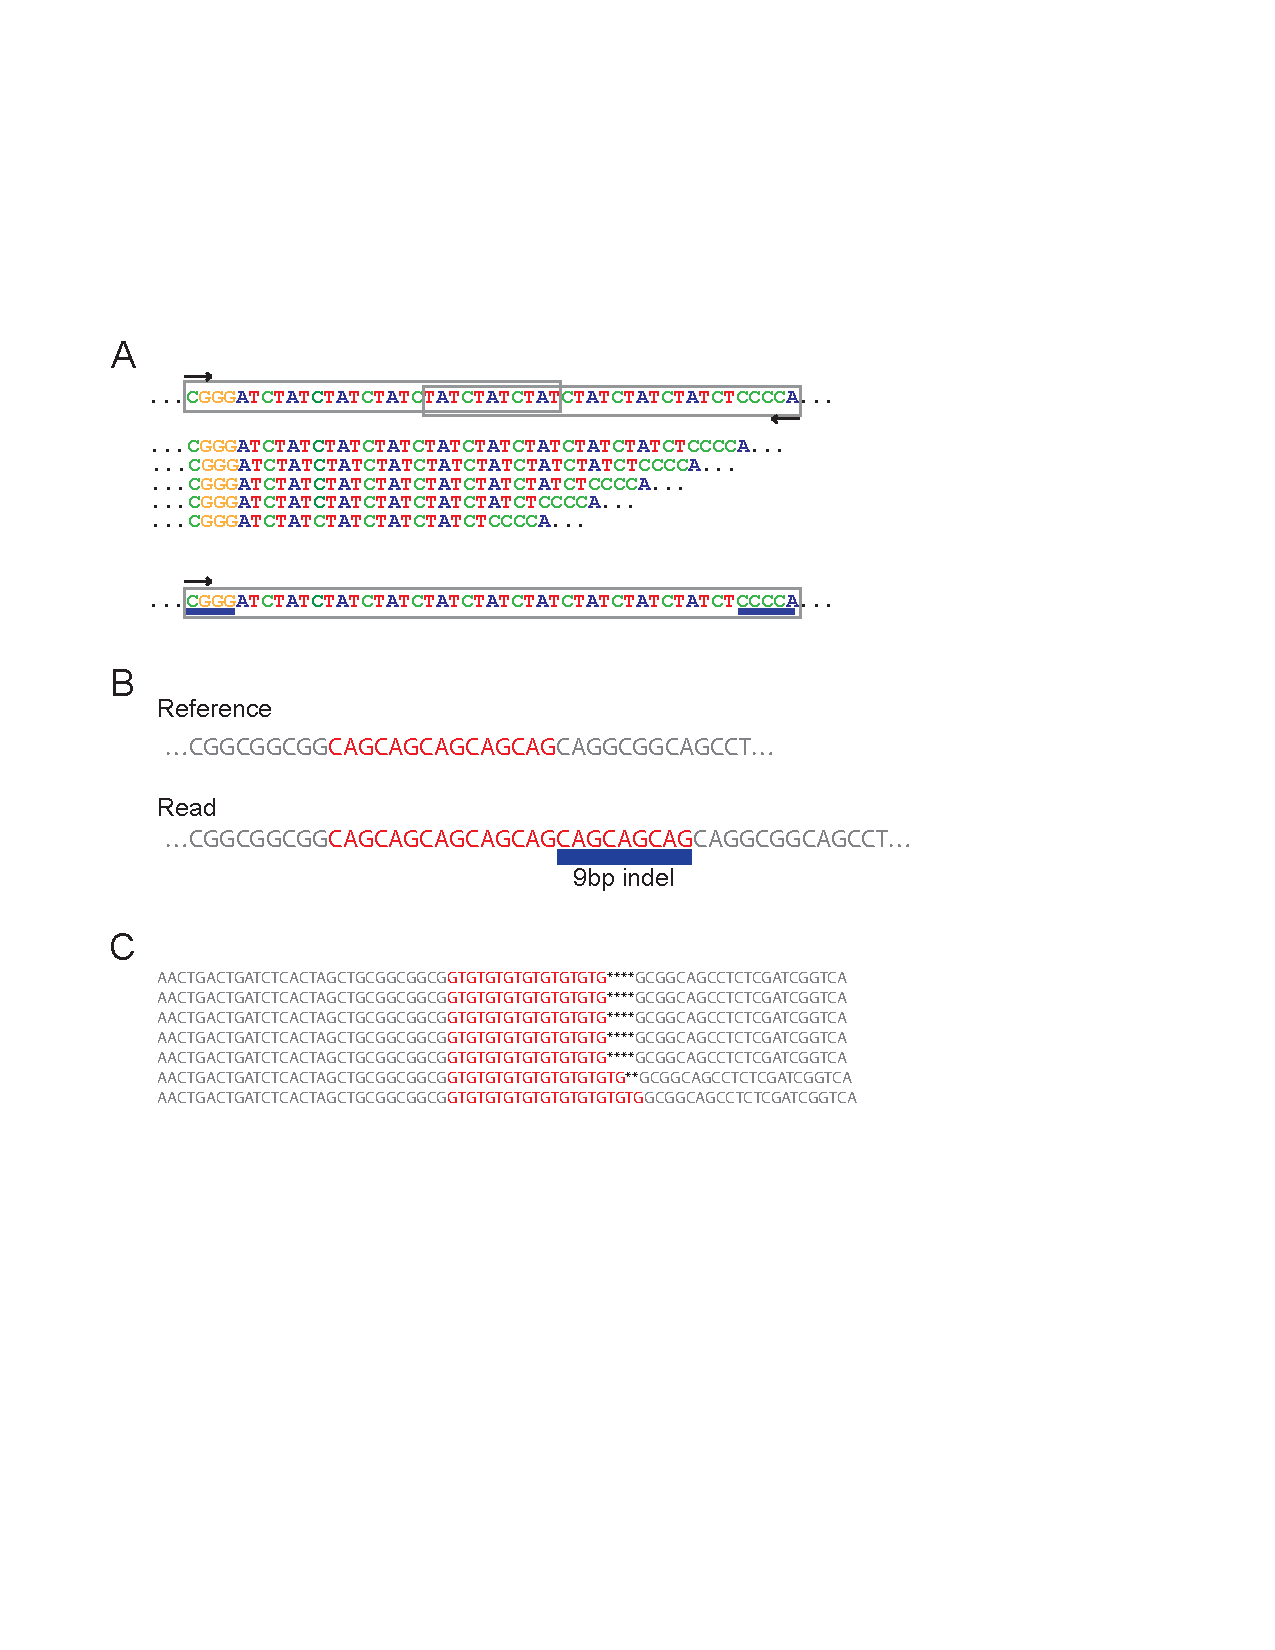
\includegraphics[width=0.65\textwidth]{Figures/Chapter2/SuppFig1.pdf}
\end{figure}
\textbf{Feasibility of STR profiling with HTS.} \textbf{(A) Long paired-end reads are not a sufficient condition for STR profiling.} Each read end (gray box) only partially covers the STR locus (top). Although the ends overlap and together span the entire locus, the number of repeat units is ambiguous (middle), since the exact overlap length is unknown. Single-ends that span the entire STR are informative (bottom). The single-end read (gray box) encompasses the flanking regions outside the STR locus (blue lines). These allow the read to be anchored to obtain unambiguous information about the STR length. \textbf{(B) Modest STR polymorphisms translate to large indels.} Thus, detecting non-reference STR reads requires cumbersome processing times by mainstream aligners \textbf{(C) An example of stutter noise due to PCR slippage events.} A series of sequence reads were obtained from the same allele. The last two reads have additional repeats due to PCR slippage events. This can confound a naive STR calling strategy to report that the locus is heterozygous.

\pagebreak
\subsection{Supplemental Figure 2}
\begin{figure}[h!]
\centering
\label{fig:lobsup2}
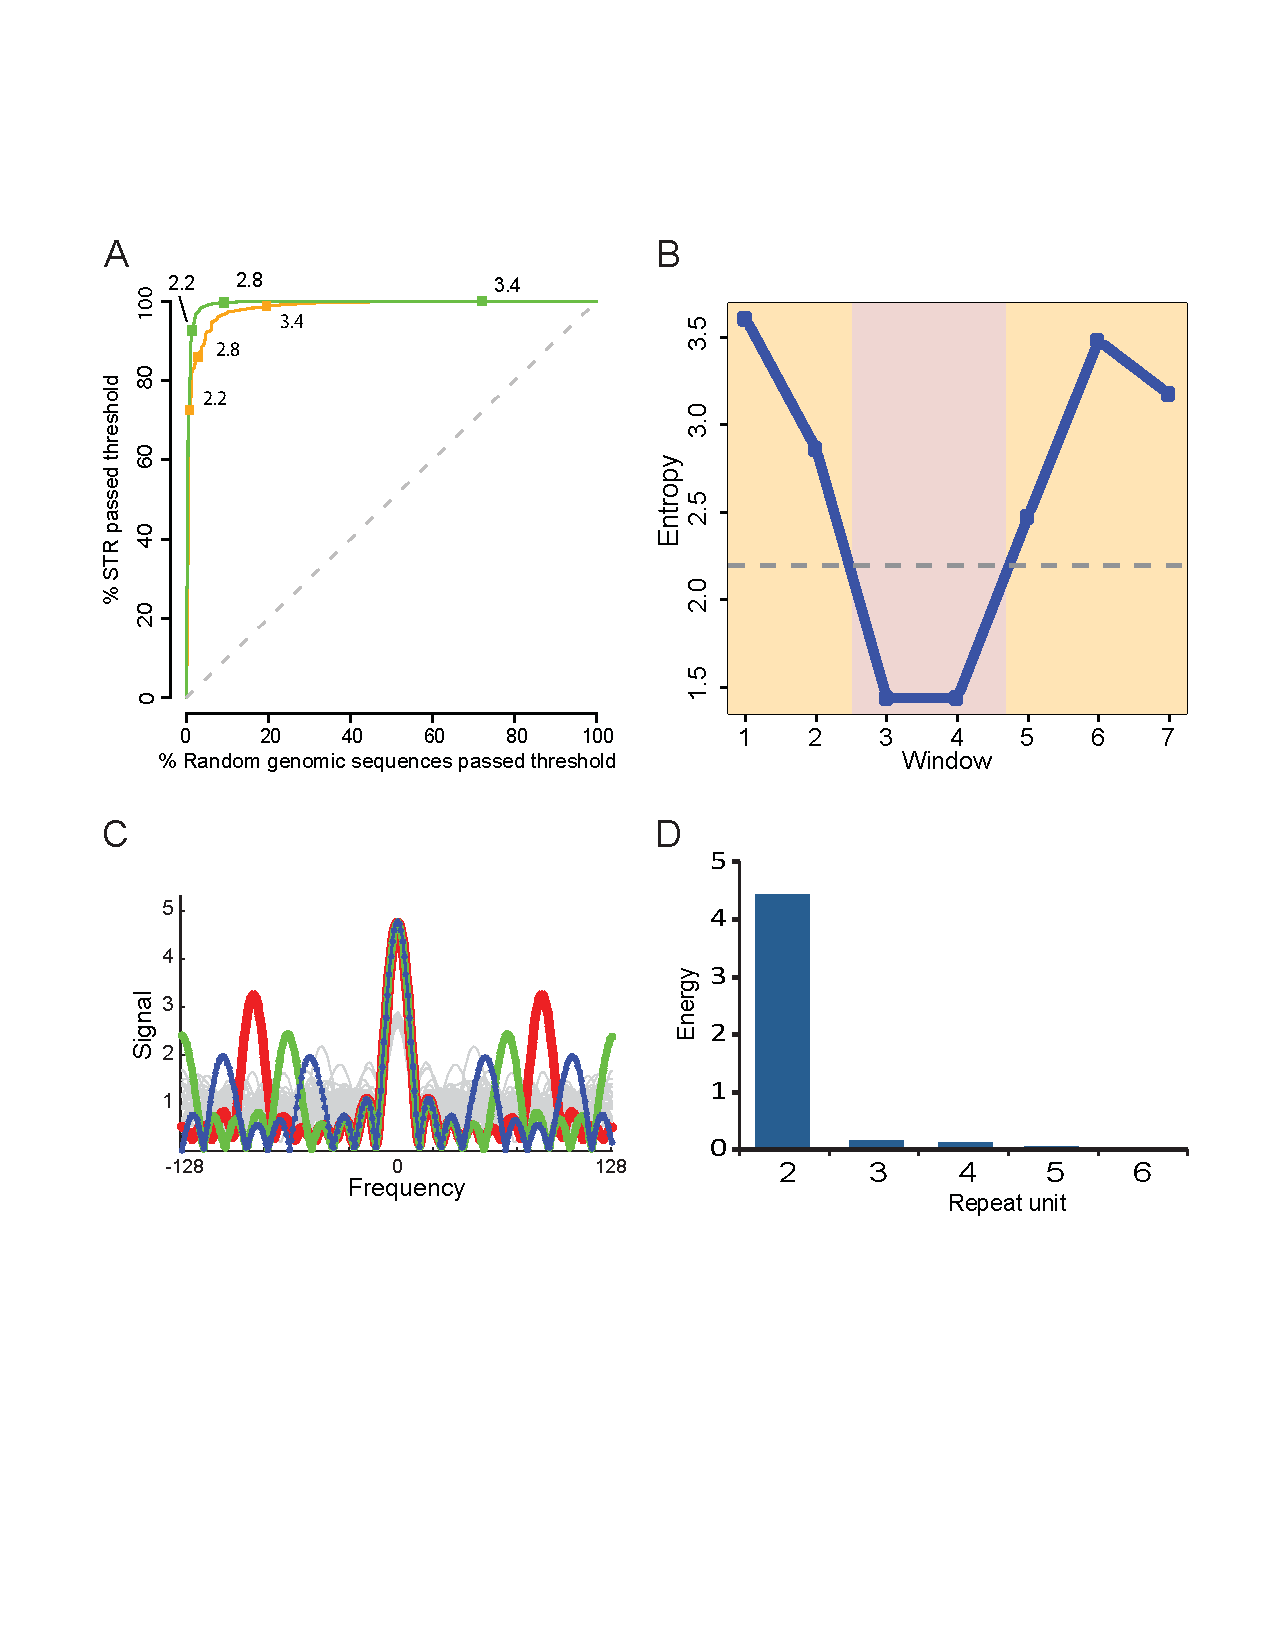
\includegraphics[width=0.65\textwidth]{Figures/Chapter2/SuppFig2.pdf}
\end{figure}
\textbf{Detection of STR containing reads} \textbf{(A) Entropy scores discriminate between STR sequences and random genomic sequences.} The receiver operating curve of the rate of STRs passing the threshold (sensitivity) versus the rate of random genomic sequences passing the threshold (1-specificity). The dinucleotide entropy (green) shows nearly perfect classification and outperforms the mononucleotide entropy (orange). The numbers on the curves denote the corresponding entropy threshold \textbf{(B) Informative reads have a unique signature in entropy analysis.} The dinucleotide entropy score is presented for sliding windows along the STR-containing sequence. The flanking regions (yellow) have a high entropy score, whereas the STR-containing region (pink) exhibits a low score. The dashed line depicts lobSTR's default entropy threshold \textbf{(C) STR periods create distinct signals in the frequency domain.} The normalized spectral response of STR repeats is characterized by distinct harmonics corresponding to the repeat unit size (blue - 5mer, green - 4mer, red - 3mer, gray - random noise) \textbf{(D) Spectral analysis determines the repeat unit length.} The period whose first harmonic shows the maximum energy is chosen as the repeat length. The example displays the normalized energies of periods 2 through 6 of a dinucleotide STR. 

\pagebreak
\subsection{Supplemental Figure 3}

\begin{figure}[h!]
\centering
\label{fig:lobsup3}
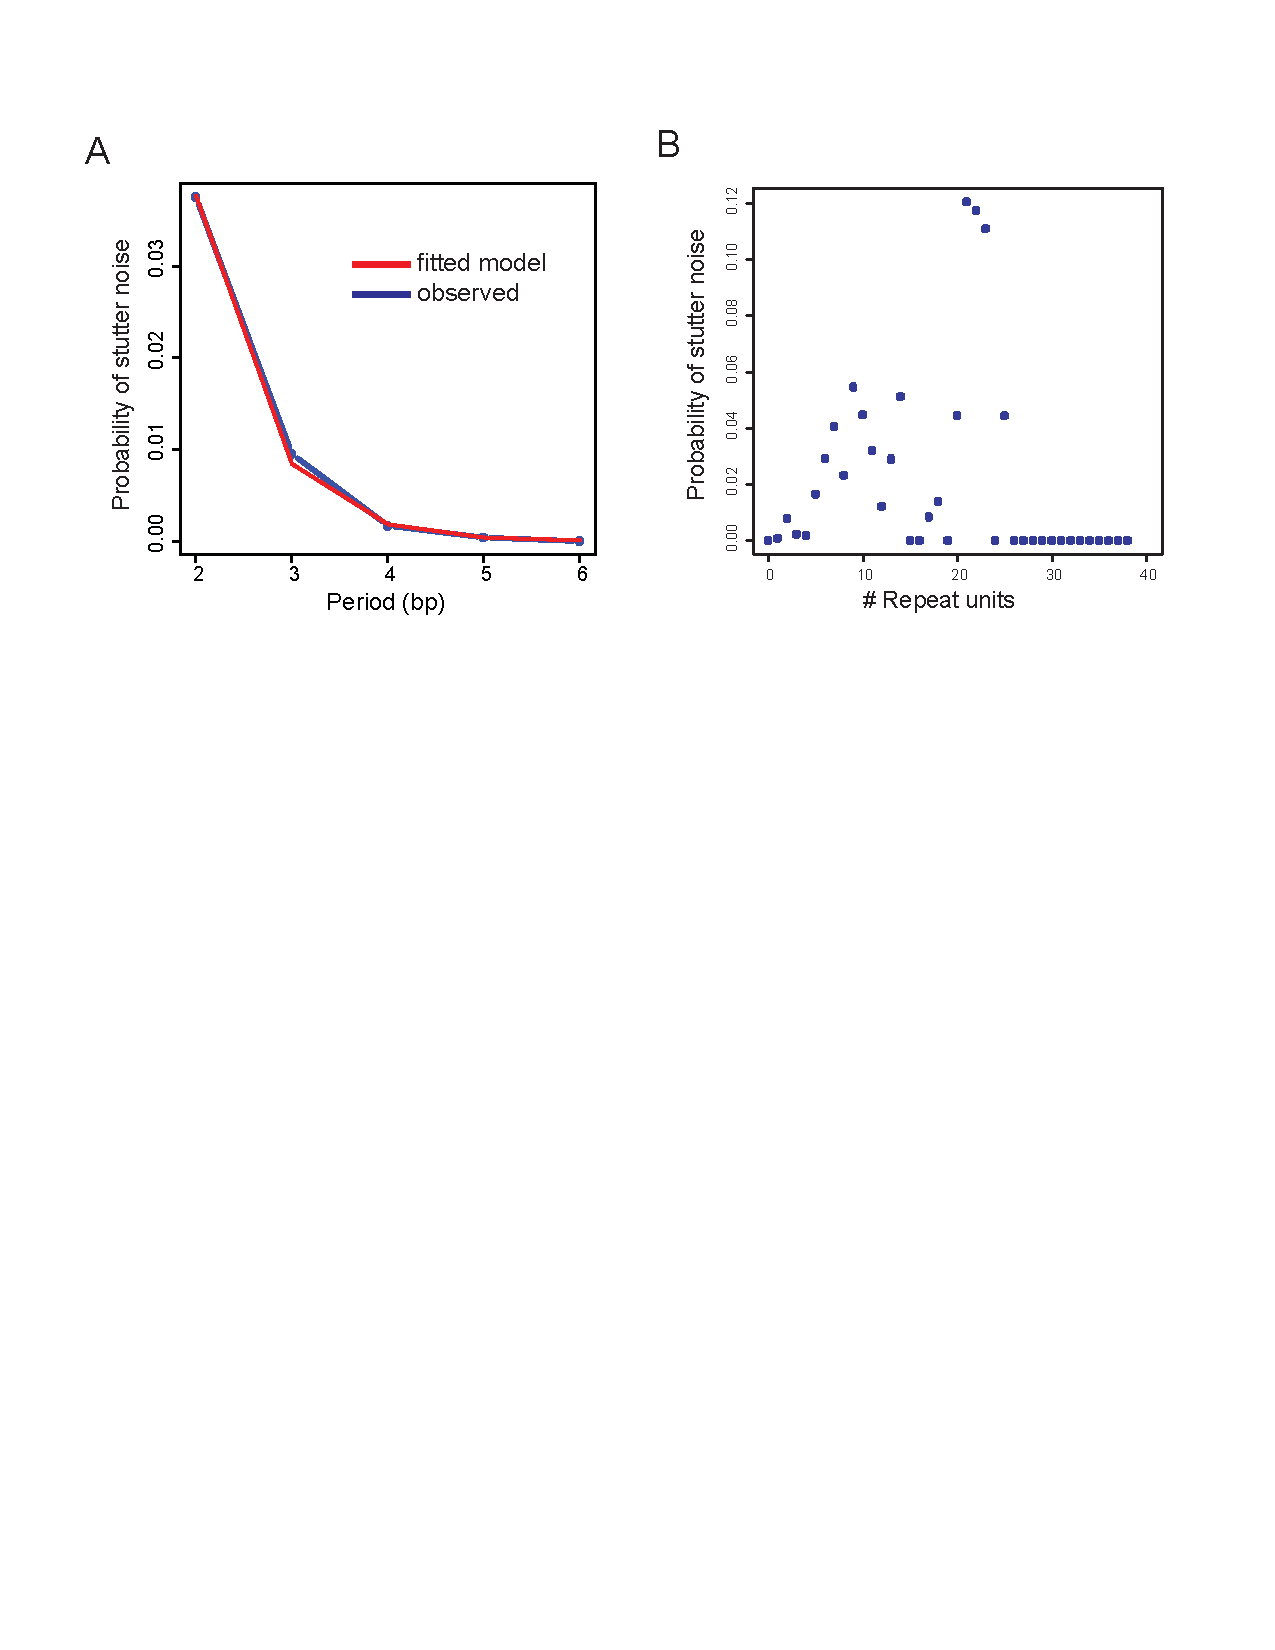
\includegraphics[width=0.7\textwidth]{Figures/Chapter2/SuppFig3.pdf}
\end{figure}
\textbf{The allelotyping step models the likelihood of PCR stutter noise.} \textbf{(A) Stutter noise as a function of STR period.} The probability of PCR stutter noise decreases with period length. Stutter noise (blue) was measured as the percentage of reads from a male sample aligned to sex chromosomes that did not exhibit the mode number of repeat units. We fitted a logistic regression (red) to model noise based on STR period. \textbf{(B) Probability of PCR stutter noise as a function of STR number.} There is no strong association between the STR region length and the stutter noise. 

\pagebreak
\subsection{Supplemental Figure 4}

\begin{figure}[h!]
\centering
\label{fig:lobsup4}
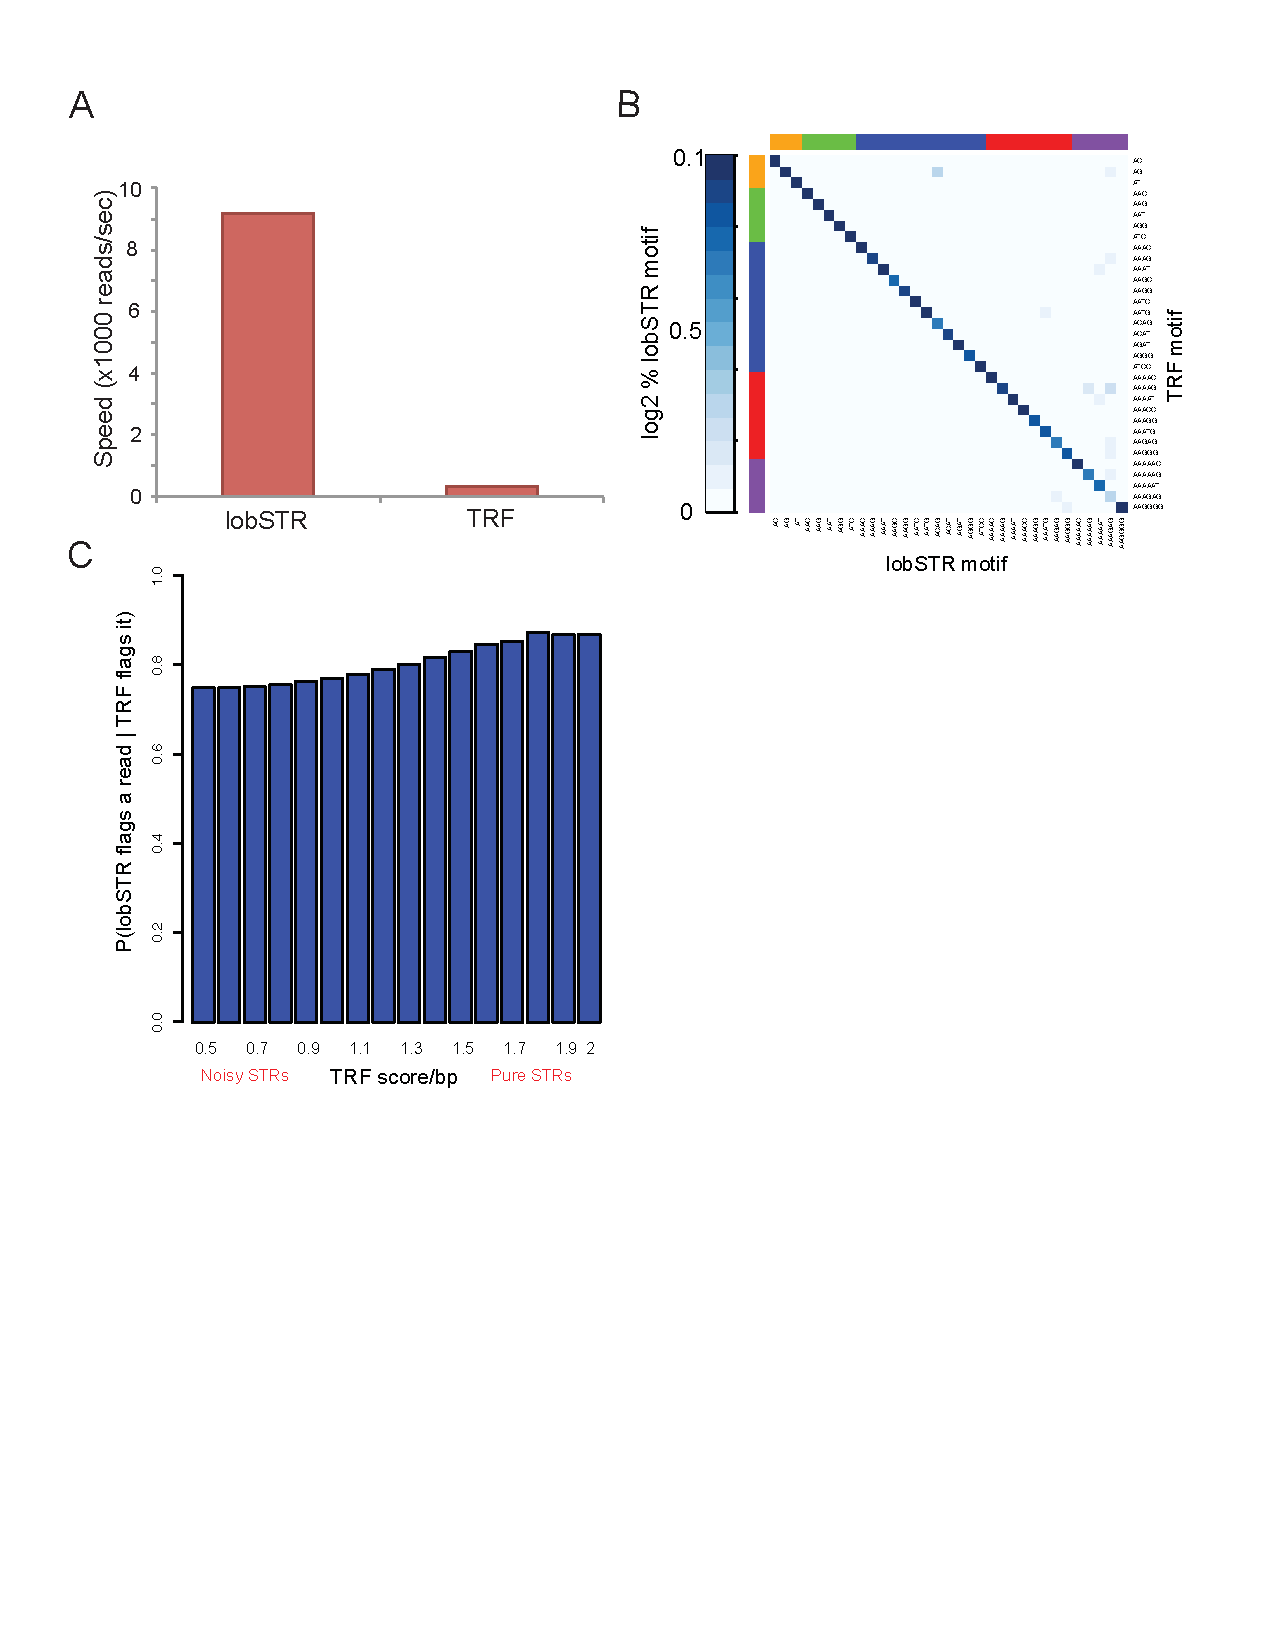
\includegraphics[width=0.7\textwidth]{Figures/Chapter2/SuppFig4.pdf}
\end{figure}
\textbf{Evaluation of the lobSTR sensing step versus TRF} \textbf{(A) lobSTR senses reads 50 times faster than TRF} \textbf{(B) lobSTR motif detection agrees with Tandem Repeat Finder.} In reads where both lobSTR and TRF detect an STR, a comparison of the most represented motifs is shown. Each column is normalized to sum to one, so that values are given in the percentage of instances of a motif detected by lobSTR that were detected as a given motif in TRF. (orange = period 2, green = period 3, blue = period 4, red = period 5, purple = period 6). Overall, lobSTR and TRF agreed in 94\% of the calls \textbf{(C) lobSTR flagging rate for reads that were flagged by TRF as a function of STR purity.} lobSTR flags about 75\% of the reads that were detected from noisy STRs and 85\% of the reads from pure STRs. 

\pagebreak
\subsection{Supplemental Figure 5}

\begin{figure}[h!]
\centering
\label{fig:lobsup5}
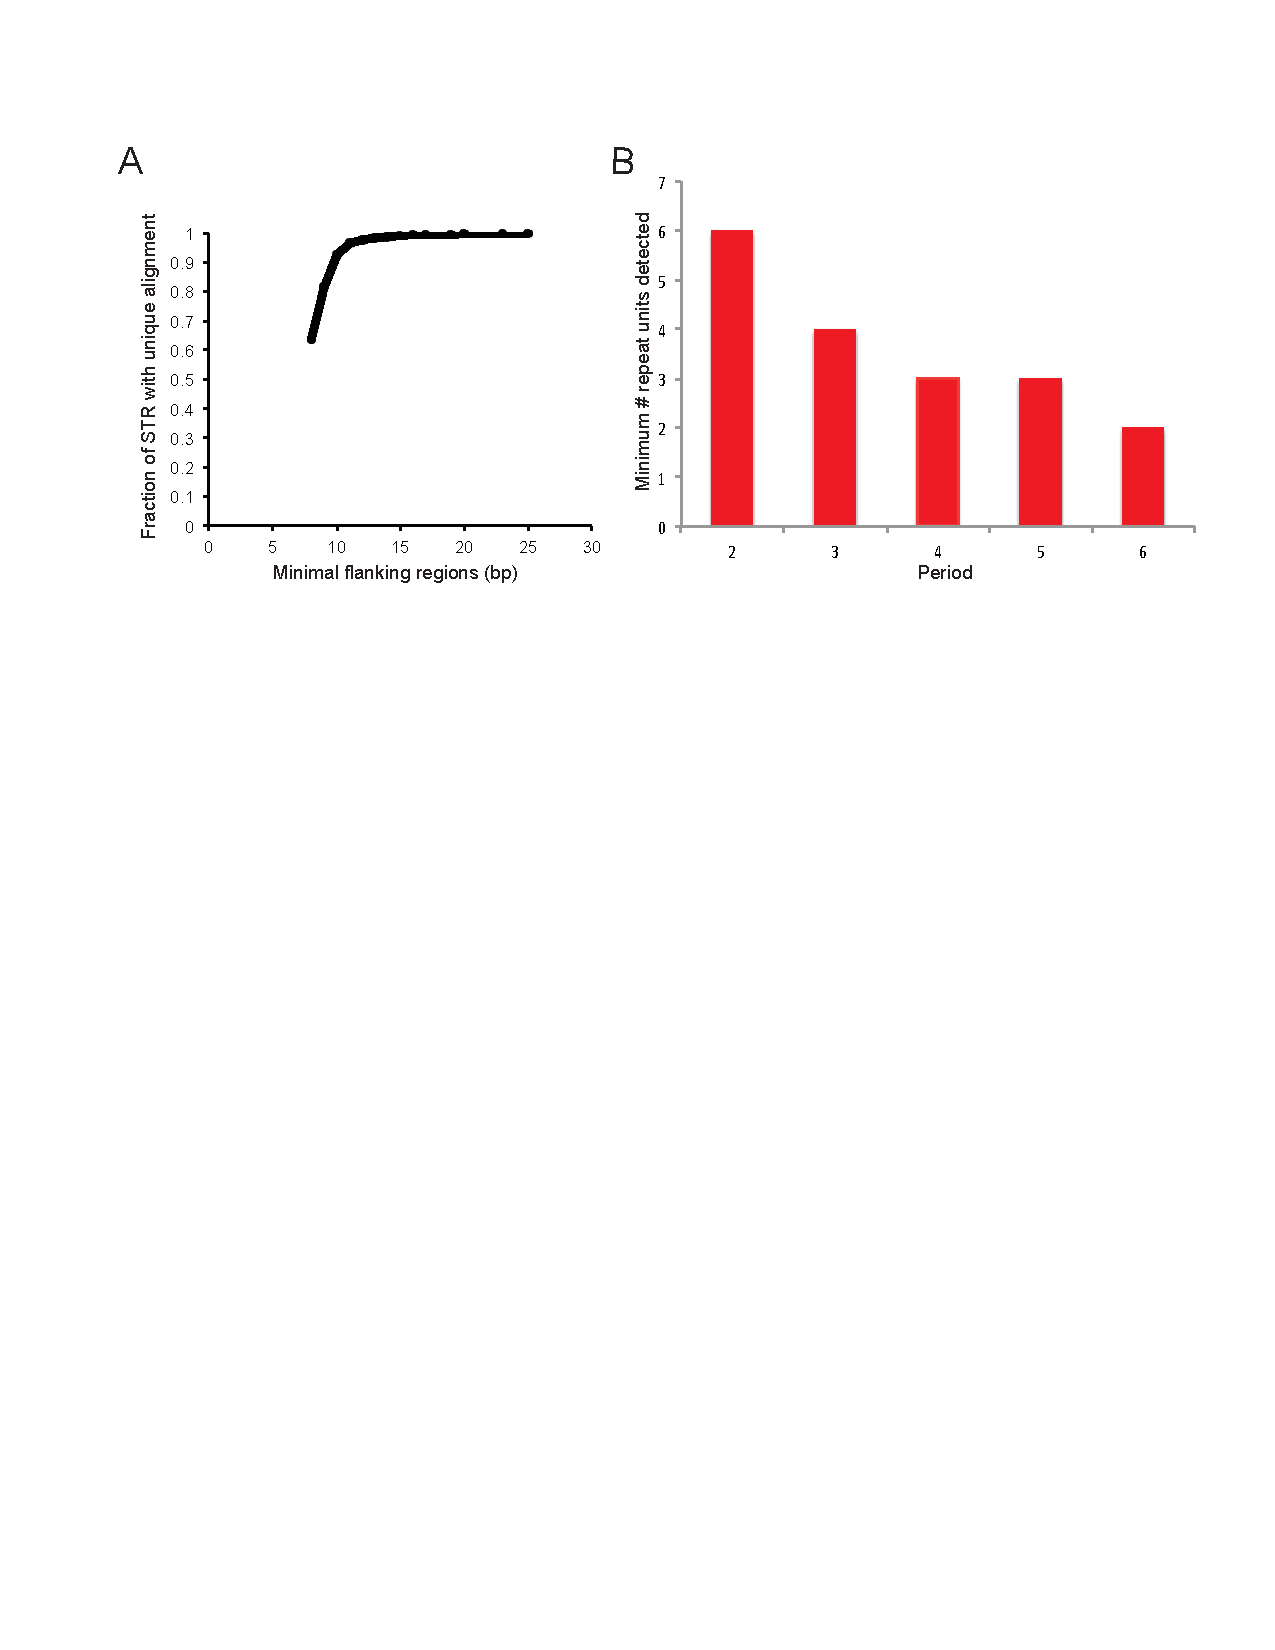
\includegraphics[width=0.7\textwidth]{Figures/Chapter2/SuppFig5.pdf}
\end{figure}
\textbf{Range of STR lengths that lobSTR can process.} lobSTR is able to process STRs with total lengths in the range of 12-84bp from 100bp reads. \textbf{(A) Mappability imposes a lower bound on the size of flanking regions for alignment.} We found that above 9bp upstream and downstream flanking regions, nearly 100\% of STR regions are uniquely aligned \textbf{(B) lobSTR can detect STRs with minimal repeat units.} lobSTR can detect STR regions spanning as few as 12 base pairs. 

\pagebreak
\subsection{Supplemental Figure 6}

\begin{figure}[h!]
\centering
\label{fig:lobsup6}
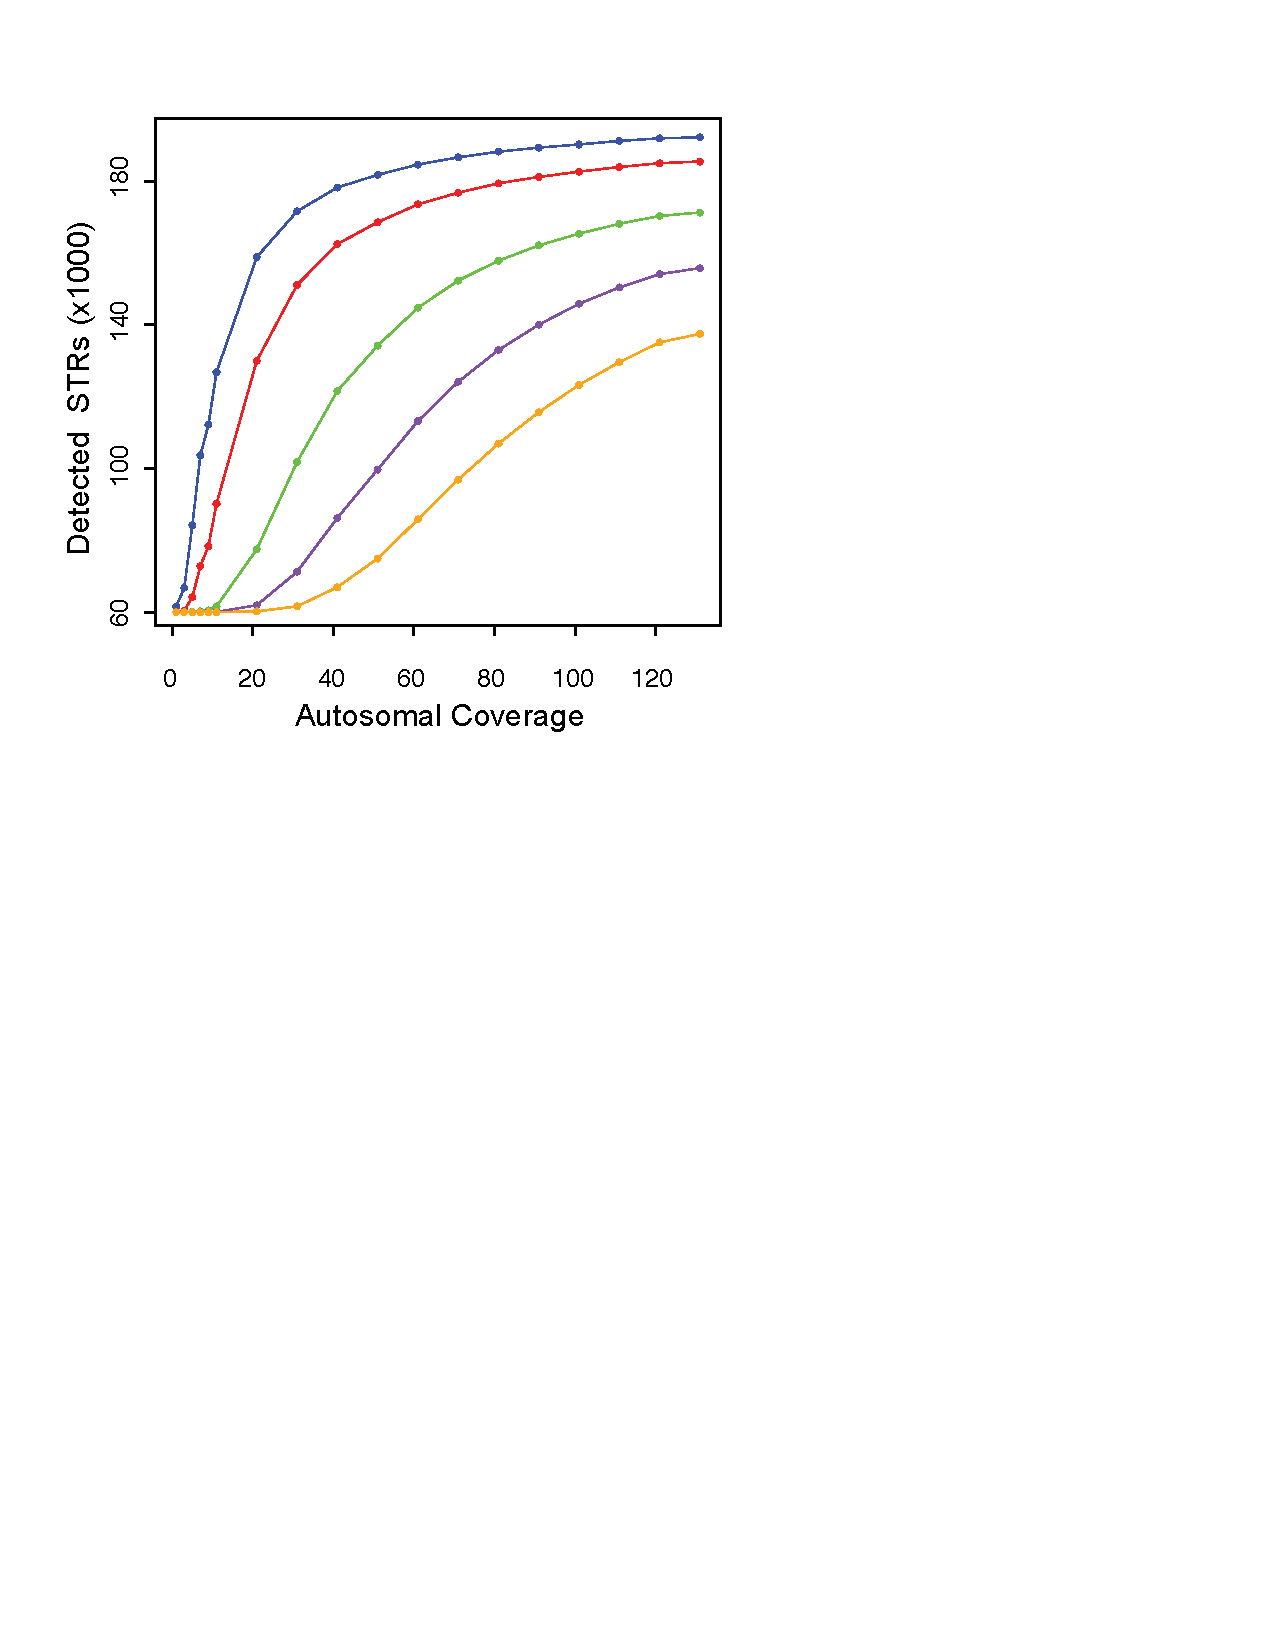
\includegraphics[width=0.7\textwidth]{Figures/Chapter2/SuppFig6.pdf}
\end{figure}
\textbf{Coverage requirements for STR allelotyping.} The number of STR loci at various STR coverage levels (blue - 3x, red - 5x, green - 10x, purple - 15x, orange - 20x) is shown as a function of autosomal genomic coverage. Various coverage levels were simulated by sampling from the aligned reads file of the 126x genome under the assumption that number of aligned STR reads is approximately proportional to genome-wide coverage.

\pagebreak
\subsection{Supplemental Figure 7}
\begin{figure}[h!]
\centering
\label{fig:lobsup7}
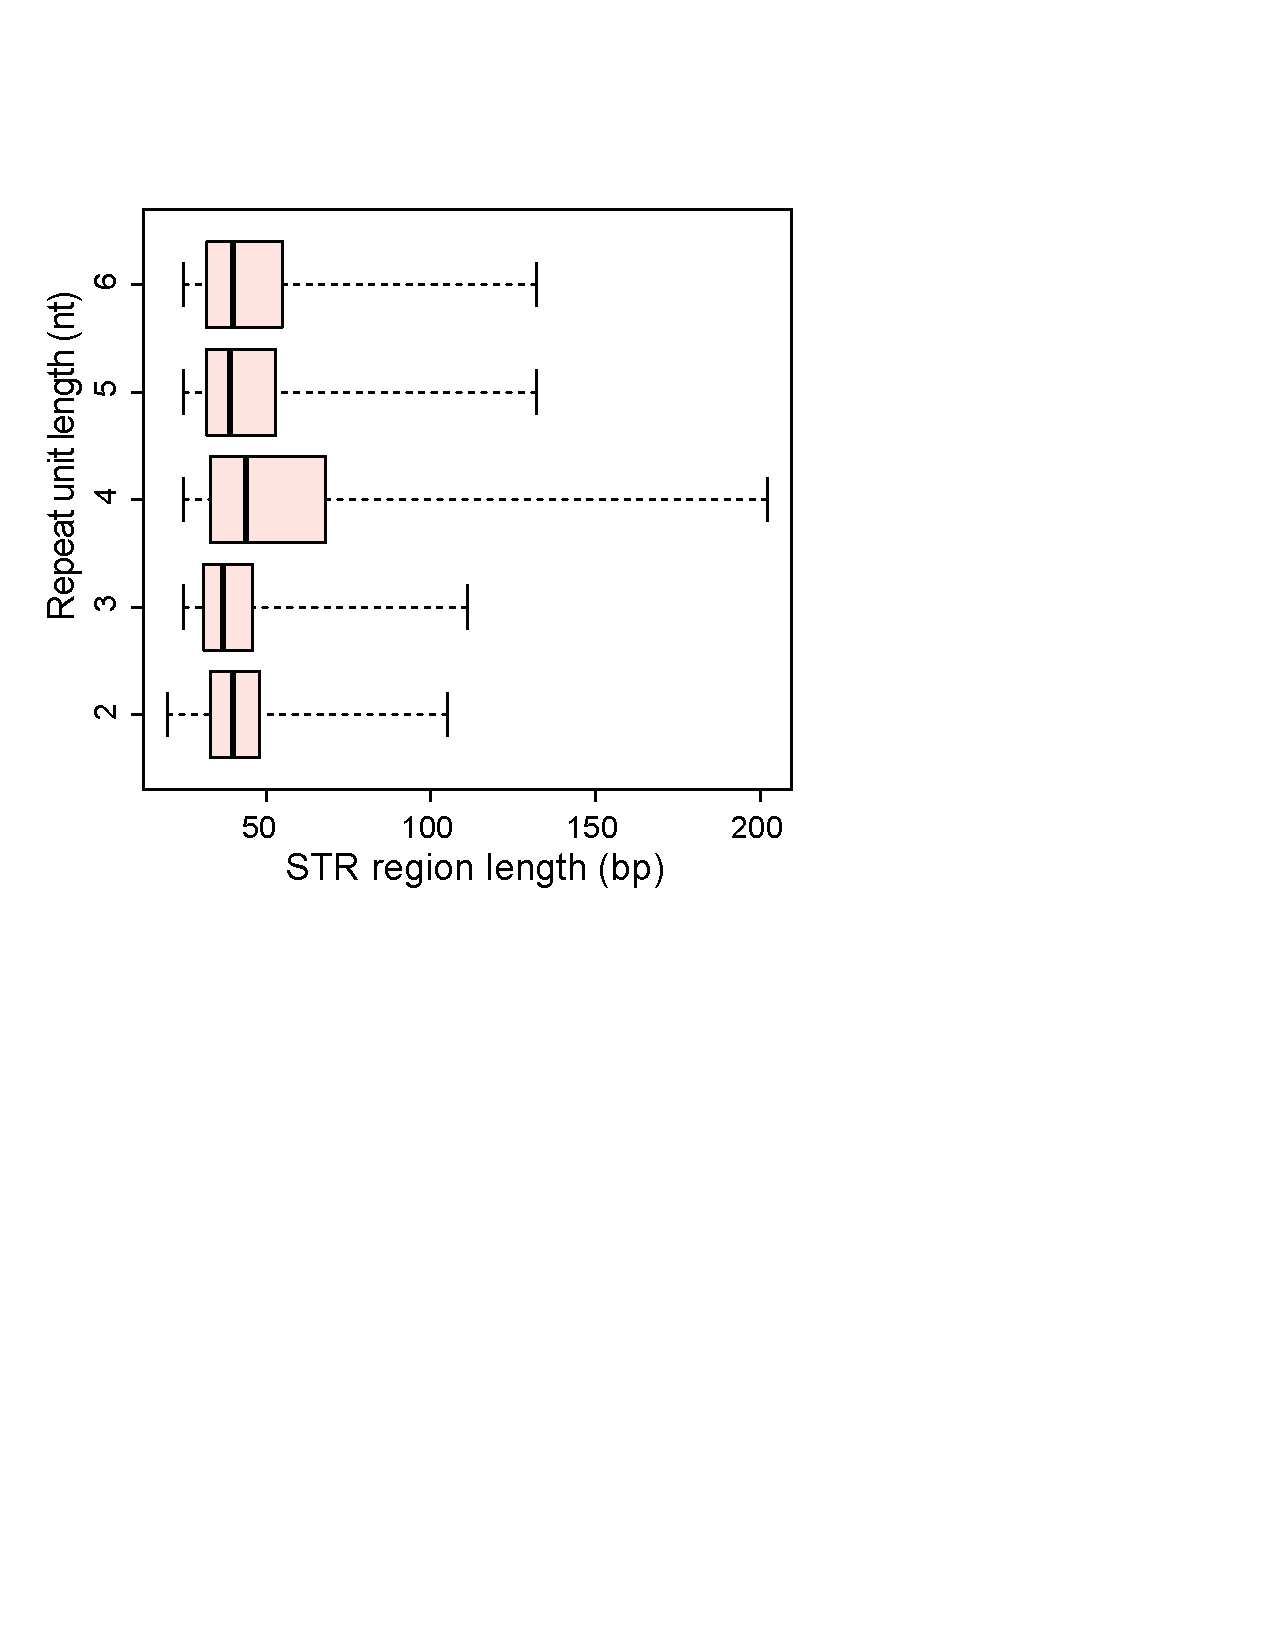
\includegraphics[width=0.7\textwidth]{Figures/Chapter2/SuppFig7.pdf}
\end{figure}
\textbf{Length distribution of STRs.} Most periods have a median STR repeat length (thick black line) of around 40bp. The repeat region total length and length variance increase slightly with increasing repeat period.
\section{Supplemental Tables}
%% TODO figures/tables and legends
\iffalse \bibliography{MGymrekRefs.bib} \fi

\chapter{The landscape of human STR variation}
\label{chap:catalog}

\hzline

Much of this chapter was first published as:

\begin{itemize}
\item[] Willems TF, \textbf{Gymrek M}, Highnam G, The 1000 Genomes Project, Mittelman D, Erlich Y. The
  Landscape of Human STR Variation. \emph{Genome Res}. (August 2014).
\end{itemize}

\hzline

\textbf{Abstract:} Short tandem repeats are among the most polymorphic loci in the human genome. These loci play a role in the etiology of a range of genetic diseases and have been frequently utilized in forensics, population genetics, and genetic genealogy. Despite this plethora of applications, little is known about the variation of most STRs in the human population. Here, we report the largest-scale analysis of human STR variation to date. We collected information for nearly 700,000 STR loci across over 1,000 individuals in phase 1 of the 1000 Genomes Project. Extensive quality controls show that reliable allelic spectra can be obtained for close to 90\% of the STR loci in the genome. We utilize this call set to analyze determinants of STR variation, assess the human reference genome's representation of STR alleles, find STR loci with common loss-of-function alleles, and obtain initial estimates of the linkage disequilibrium between STRs and common SNPs. Overall, these analyses further elucidate the scale of genetic variation beyond classical point mutations.

\section{Introduction}
STRs are abundant repetitive elements that are comprised of recurring DNA motifs of 2- 6 bases. These loci are highly prone to mutations due to their susceptibility to slippage events during DNA replication \cite{Ellegren2004}. To date, STR mutations have been linked to at least 40 monogenic disorders \cite{PearsonNicholEdamuraCleary2005,Mirkin2007}, including a range of neurological conditions such as Huntington's disease, amyotrophic lateral sclerosis, and certain types of ataxia. Some disorders, such as Huntington's disease, are triggered by the expansion of a large number of repeat units. In other cases, such as oculopharyngeal muscular dystrophy, the pathogenic allele is only two repeat units away from the wild-type allele \cite{BraisBouchardXieEtAl1998}. In addition to Mendelian conditions, multiple studies have suggested that STR variations contribute to an array of complex traits \cite{GemayelVincesLegendreEtAl2010}, ranging from the period of the circadian clock in Drosophila \cite{SawyerHennessyPeixotoEtAl1997} to gene expression in yeast \cite{VincesLegendreCaldaraEtAl2009} and splicing in humans \cite{HefferonGromanYurkEtAl2004,SathasivamNeuederGipsonEtAl2013}.

Beyond their importance to medical genetics, STR variations convey high information content due to their rapid mutations and multi-allelic spectra. Population genetics studies have utilized STRs in a wide-range of methods to find signatures of selection and to elucidate mutation patterns in nearby SNPs \cite{TishkoffVarkonyiCahinhinanEtAl2001,SunHelgasonMassonEtAl2012}. In DNA forensics, STRs play a significant role as both the US and the European forensic DNA databases rely solely on these loci to create genetic fingerprints \cite{KayserKnijff2011}. Finally, the vibrant genetic genealogy community extensively uses these loci to develop impressive databases containing lineages for hundreds of thousands of individuals \cite{KhanMittelman2013}.

Despite their utility, systematic data about the landscape of STR variations in the human population is far from comprehensive. Currently, most of the genetic information concerns a few thousand loci that were part of historical STR linkage and association panels in the pre SNP-array era \cite{BromanMurraySheffieldEtAl1998,TamiyaShinyaImanishiEtAl2005} and several hundred loci involved in forensic analysis, genetic genealogy, or genetic diseases \cite{RuitbergReederButler2001,PearsonNicholEdamuraCleary2005}. In total, there are only 5,500 loci under the microsatellite category in dbSNP139. For the vast majority of STR loci, little is known about their normal allelic ranges, frequency spectra, and population differences. This knowledge gap largely stems from the absence of high-throughput genotyping Downloaded from genome.cshlp.org on December 8, 2015 - Published by Cold Spring Harbor Laboratory Press techniques for these loci \cite{JorgensonWitte2007}. Capillary electrophoresis offers the most reliable method to probe these loci, but this technology scales poorly. More recently, several studies have begun to genotype STR loci with whole-genome sequencing datasets obtained from long read platforms such as Sanger sequencing \cite{PayseurJingHaasl2011} and 454 \cite{MollaDelcherSunyaevEtAl2009}. However, due to the relatively low throughput of these platforms, these studies analyzed STR variations in only a few genomes.

Illumina sequencing has the potential to profile STR variations on a population-scale. However, STR variations present significant challenges for standard sequence analysis frameworks \cite{TreangenSalzberg2012}. In order to reduce computation time, most alignment algorithms employ heuristics that reduce their tolerance to large indels, hampering alignment of STRs with large contractions or expansions. In addition, due to the repetitive nature of STRs, the PCR steps involved in sample preparation induce in vitro slippage events \cite{HaugeLitt1993}. These events, called stutter noise, generate erroneous reads that mask the true genotypes. Because of these issues, previous largescale efforts to catalog genetic variations have omitted STRs from their analyses \cite{AbecasisAltshulerAutonEtAl2010} and early attempts to analyze STRs using the 1000 Genomes data were mainly focused on exonic regions \cite{McIverFondonSkinnerEtAl2011} or extremely short STR regions with a relatively small number of individuals based on the native indel callset \cite{AnandaWalshJacobEtAl2012}.

In our previous studies, we created publicly available programs that specialize in STR profiling using Illumina whole-genome sequencing data \cite{GymrekGolanRossetEtAl2012,HighnamFranckMartinEtAl2013}. Recently, we deployed one of these tools (lobSTR) to accurately genotype STRs on the Y chromosome of anonymous individuals in the 1000 Genomes Project to infer their surnames \cite{GymrekMcGuireGolanEtAl2013}, demonstrating the potential utility of STR analysis from Illumina sequencing. Here, we used these tools to conduct a genome-wide analysis of STR variation in the human population using the sequencing data of the Phase 1 of the 1000 Genome Project.

\section{Results}
\subsection{Identifying STR loci in the human genome}
The first task in creating a catalog of STR variation is to determine the loci in the human reference that should be considered as STRs. This problem primarily stems from the lack of consensus in the literature as to how many copies of a repeat distinguish an STR from genomic background \cite{LeclercqRivalsJarne2007,FondonMartinRichardsEtAl2012,SchaperKajavaHauserEtAl2012}. For example, is $(AC)_2$ an STR? What about $(AC)_3$ or $(AC)10$? Furthermore, as sporadic bases can interrupt repetitive DNA sequences, purity must also be taken into account when deciding whether a locus is a true STR.  

We employed a quantitative approach to identify STR loci in the reference genome. Multiple lines of study have proposed that the birth of an STR is a relatively rare event with complex biology \cite{Ellegren2004,GemayelVincesLegendreEtAl2010,AnandaWalshJacobEtAl2012,BuschiazzoGemmell2006,OliverSlashinskiWangEtAl2012,KelkarEckertChiaromonteEtAl2011}. The transition from a proto-STR to a mature STR requires non-trivial mutations such as the arrival of a transposable element, slippage-induced expansion of the proto-STR, or precise point mutations that destroy non-repetitive gaps between two short repeat stretches. Based on these observations, it was suggested that randomly-shuffled DNA sequence should rarely produce mature STR sequences and therefore can be used as negative controls for STR discovery algorithms \cite{GemayelVincesLegendreEtAl2010,SchaperKajavaHauserEtAl2012}. We utilized this approach to identify STR loci in the human genome while controlling the false positive rate \cite{SuppWillemsGymrekHighnamEtAl2014}. We first integrated the purity, composition, and length of putative STRs in the genome into a score using Tandem Repeats Finder [TRF] \cite{Benson1999}. Then, we generated random DNA sequences using a second-order Markov chain with similar properties to the human genome (i.e. nucleotide composition and transition frequencies). We tuned the TRF score threshold such that only 1\% of the identified STR loci in our collection were expected to be false positives. The resulting score thresholds were in good qualitative agreement with those previously produced using a variety of alternative experimental and analytical methods \cite{LaiSun2003,FondonMartinRichardsEtAl2012,KelkarStrubczewskiHileEtAl2010} \cite{SuppWillemsGymrekHighnamEtAl2014}. We then evaluated the false negative rate of our catalog using two methods \cite{SuppWillemsGymrekHighnamEtAl2014}. First, we collected a preliminary call set of repeat number variability across the human population with a highly permissive definition of STR loci. We found that our catalog misses only $\sim 1$\% of loci that exhibited repeat variability in the permissive call set \cite{SuppWillemsGymrekHighnamEtAl2014}. Second, we also collated a set of about 850 annotated bona-fide STR loci, mainly from the CODIS forensic panel and Marshfield linkage panel. Only 12 (1.4\%) of these markers were not included in the catalog based on the TRF score threshold. The results of the two validation methods suggest that our catalog includes $\sim$99\% of the true STRs in the genome and has a false negative rate of about 1\%. 

Overall, our STR reference includes approximately 700,000 loci in the human genome. About 75\% of these loci are di and tetra-nucleotide STRs, while the remaining loci are tri, penta and hexa-nucleotide STRs \cite{SuppWillemsGymrekHighnamEtAl2014}. Approximately 4,500 loci overlap coding regions, 80\% of which have either trimeric or hexameric repeat units.  In addition, the reference contains a roughly equal proportion of interrupted and uninterrupted microsatellites.  

\subsection{Profiling STRs in 1000 Genomes samples}
We collected variations for these 700,000 STR loci using 1,009 individuals from phase 1 of the 1000 Genomes Project (\textbf{Methods \ref{sec:catmet}, \cite{SuppWillemsGymrekHighnamEtAl2014}}). These samples span populations from five continents and were subject to low coverage ($\sim$5x) whole-genome sequencing using 76bp and 100bp Illumina paired-end reads. In addition, high coverage exome sequencing data was available for 975 of these samples and was integrated with the whole-genome raw sequencing files.  

We tested two distinct STR genotyping pipelines designed to analyze high-throughput sequencing data, namely lobSTR \cite{GymrekGolanRossetEtAl2012} and RepeatSeq \cite{HighnamFranckMartinEtAl2013}. Briefly, lobSTR utilizes the non-repetitive flanking regions surrounding STRs to align reads and assess their allele lengths, while RepeatSeq utilizes Bayesian model selection to genotype previously aligned STR-containing reads. Despite significant methodological differences, the STR genotypes from the two tools were quite concordant and matched for 133,375,900 (93\%) out of the 143,428,544 calls that were reported by both tools. We tested multiple methods to unify the two call sets in order to further improve the quality \cite{SuppWillemsGymrekHighnamEtAl2014}. However, none of these integration methods improved the accuracy. Since the lobSTR calls showed better quality for highly polymorphic STRs, we proceeded to analyze STR variations using only this call set.  

On average, we collected STR genotypes for approximately 530 individuals per locus (\textbf{Figure \ref{fig:catfig1}a}) and 350,000 STR loci per individual (\textbf{Figure \ref{fig:catfig1}b}), accumulating a total of about 350 million STR genotypes in the catalog. We examined the marginal increase in the number of covered STR loci as a function of sample size (\textbf{Methods \ref{sec:catmet}, Figure \ref{fig:catfig1}c}). Our analysis shows that after analyzing 100 samples, there is a negligible increase in the number of genotyped STRs. However, even with all of the data, 3\% of STR loci are persistently absent from the catalog. The average reference allele length of the missing STR loci was 182bp compared to 31bp for the rest of the reference, suggesting that the missing STR loci have allele lengths beyond the read length of Illumina sequencing. We also examined the marginal increase of polymorphic STR loci with minor allele frequencies (MAF) greater than 1\%. Again, we observed an asymptote after approximately 100 samples. These saturation analyses suggest that with the current sample size, the STR variation catalog virtually exhausted all loci with MAF$>$1\% that can be observed with 100bp Illumina reads and our analysis pipeline.  

\begin{figure}[h!]
\centering
\label{fig:catfig1}
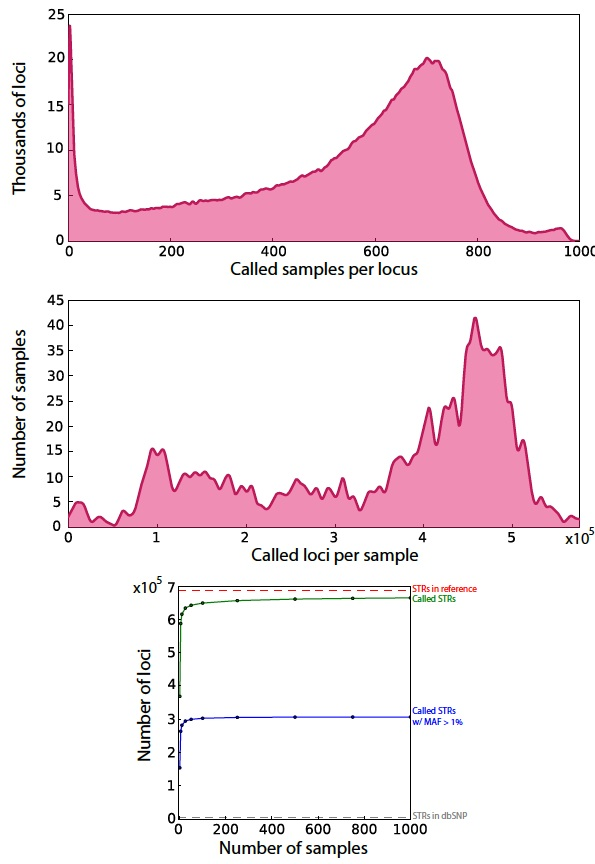
\includegraphics[width=0.5\textwidth]{Figures/Chapter3/Fig1.jpg}
\caption{\textbf{Call set statistics} \textbf{(A) Distribution of the number of called samples per locus.} The average is 528 samples per STR with a standard deviation of 231 \textbf{(B) Distribution of the number of called loci per sample.} The average is 349,892 STR per sample with a standard deviation of 145,135 \textbf{(C) Saturation curves for the catalog.} The number of called loci (green) rapidly approaches the total number of STRs in the genome (red line). The number of called loci with a MAF$>$1\% (blue) saturates after 100 samples and far exceeds the number of STR variants in dbSNP (grey line close to the Xaxis).}
\end{figure}

The full catalog of STR variations is publicly available at \url{http://strcat.teamerlich.org} in VCF format. In addition, the website provides a series of graphical interfaces to search for STR loci with specific biological properties such as distance to splice sites, obtain summary statistics such as allelic spectrum and heterozygosity rates, and view the supporting raw sequencing reads. 

\subsection{Quality assessment}
To initially assess the accuracy of our STR calls, we first examined patterns of Mendelian inheritance (MI) of STR alleles for three low-coverage trios present in the sample set. In total, we accumulated half a million genotypes calls. Without any read depth threshold, 94\% of the STR loci followed MI (\textbf{Figure \ref{fig:catfig2}a}). The MI rates increased monotonically with read depth and restricting the analysis to loci with at least ten reads increased the Mendelian inheritance to over 97\%.  

Next, we compared the concordance of the calls in our catalog to those obtained using capillary electrophoresis, the gold standard for STR calling (\textbf{Methods \ref{sec:catmet}}). We focused on datasets containing Marshfield and PowerPlex Y chromosome panel genotypes that are available for a subset of the 1000 Genomes individuals. These panels ascertain some of the most polymorphic STR loci, testing our pipeline in a challenging scenario. The Marshfield capillary panel \cite{Rosenberg2006} reported 5,164 genotypes that overlapped with the lobSTR calls and pertained to 157 autosomal STRs and 140 individuals, while the PowerPlex capillary panel reported 784 genotypes that overlapped with the lobSTR calls and pertained to 17 Y-STRs and 228 individuals.  

One key question is finding an adequate cost function to assess the concordance between the STR calls. In SNPs, the proportion of mismatches is a natural measure of concordance due to their binary nature. However, for STRs, this approach assigns the same penalty for missing one repeat unit and ten repeat units. As an alternative, we focused on measuring the goodness-of-fit ($R^2$) between the STR dosages. The dosage of an STR was defined as the sum of the number of base pairs after subtracting the reference allele. For example, if the genotype was 16bp/18bp and the reference allele was 14bp, the dosage of the locus was set to 2+4=6, while for hemizygous loci the dosage was the difference from the reference allele. We focused on assessing dosage concordance because of the growing body of studies suggesting that the phenotypic impact of STRs is strongly correlated with length \cite{GebhardtZankerBrandt1999,ShimajiriArimaTanimotoEtAl1999,ContenteDittmerKochEtAl2002,HefferonGromanYurkEtAl2004}. $R^2$ confers the property that the cost is proportional to the (squared) magnitude of the error in terms of length. In addition, the $R^2$ of the dosages measures the amount of genetic variance that was recovered by lobSTR under strict additivity, which might be important for downstream association studies. 

After regressing the lobSTR dosages with the capillary dosages, the resulting goodness of fit estimators ($R^2$) were 0.71 for the autosomal genotypes and 0.94 for the Y chromosome genotypes (\textbf{Figure \ref{fig:catfig2}b; \cite{SuppWillemsGymrekHighnamEtAl2014}}). By further stratifying the autosomal calls by the capillary genotype, we found that lobSTR correctly reported 89.5\% of all homozygous loci and recovered one or more alleles for 91.5\% of all heterozygous loci, but only correctly reported both alleles for 12.8\% of all heterozygous loci \cite{SuppWillemsGymrekHighnamEtAl2014}. For the Y chromosome, 95\% of the lobSTR genotypes exactly matched the capillary genotypes for the PowerPlex Y panel \cite{SuppWillemsGymrekHighnamEtAl2014}. 

Collectively, these results suggest that the individual allele lengths are relatively accurate and that the primary source of noise is the recovery of only one STR allele for heterozygous loci, an issue known as allelic dropout. This statement is supported by the relatively good accuracy achieved for the homozygous autosomal loci and hemizygous Y chromosome loci, and the monotonically increasing relationship between heterozygote accuracy and read depth, with a heterozygote accuracy of nearly 80\% achieved for loci covered by 6 or more reads (Supplemental Figure 4). In general, allelic dropouts are quite expected given the relatively low sequencing coverage but are also known to be an issue in genotyping STRs with capillary electrophoresis \cite{PompanonBoninBellemainEtAl2005}.   

We performed various analyses that demonstrate that allelic dropouts do not hamper the ability to deduce population-scale patterns of human STR variation. First, we examined the concordance of heterozygosity rates obtained from the lobSTR and the capillary calls for Marshfield STRs in three European subpopulations (CEU, GBR and FIN). The heterozygosity rate is based on the frequency spectrum of a locus (\textbf{Methods \ref{sec:catmet}}) and should be unaffected by random allelic dropout. As expected, we found that the heterozygosity rates were highly similar between the capillary and the lobSTR results (\textbf{Figure \ref{fig:catfig2}c}). The regression slope was 0.996 and the root mean squared error (RMSE) was 0.044 based on over 200 STRs. This analysis shows that the heterozygosity estimates obtained from our call set are relatively unbiased. 

We also benchmarked the quality of population-scale patterns by comparing the allelic spectra for the Marshfield loci \cite{SuppWillemsGymrekHighnamEtAl2014}. We found that in most cases, the lobSTR and capillary spectra matched in the median and interdecile range of the reported allelic lengths. We also inspected the frequency spectra of STRs that are part of the forensic CODIS test panel using a similar procedure (\textbf{Figure \ref{fig:catfig2}d; \cite{SuppWillemsGymrekHighnamEtAl2014}}). A previous study reported the spectra of these loci by genotyping $\sim$200 Caucasians in the United States using capillary electrophoresis \cite{BudowleSheaNiezgodaEtAl2001}. Again, these comparisons resulted in similar patterns for eight of the ten analyzed markers. We found marked biases only for FGA and D18S51, with lobSTR reporting systematically shorter alleles. As the maximal allele sizes of these two loci are over 80bp, the long alleles are seldom spanned by the mixture of 76 and 100 bp Illumina reads in Phase 1, creating a bias toward shorter alleles.  

We sought to further characterize potential biases towards ascertaining shorter alleles with lobSTR and the 76bp/100bp Illumina reads. To that end, we inspected the concordance between the lobSTR calls and the NCBI reference (\textbf{Figure \ref{fig:catfig2}e}). The NCBI reference was generated by long Sanger reads and therefore should be an unbiased estimator of the most common allele in the population. In the absence of any systematic bias towards shorter alleles, the expected deviation of a lobSTR allele from the NCBI reference should be zero. On the other hand, in the presence of such a bias, the lobSTR calls should be systematically smaller than the NCBI reference and generate a negative deviation. We found that the median deviation of lobSTR was around zero for STRs with reference alleles up to 45bp. Above this threshold, we started to observe systematic deviations towards shorter alleles. The deviation did not monotonically decrease but exhibited a local maximum around 65bp, which presumably stems from the heterogeneity of the sequencing read lengths and the exhaustion of alleles that can be spanned by 76bp reads. Importantly, only 10\% of all loci in our catalog have a reference allele greater than 45bp. This implies that for the vast majority of the loci, the allelic spectra are expected to be unbiased.  

\begin{figure}[h!]
\centering
\label{fig:catfig2}
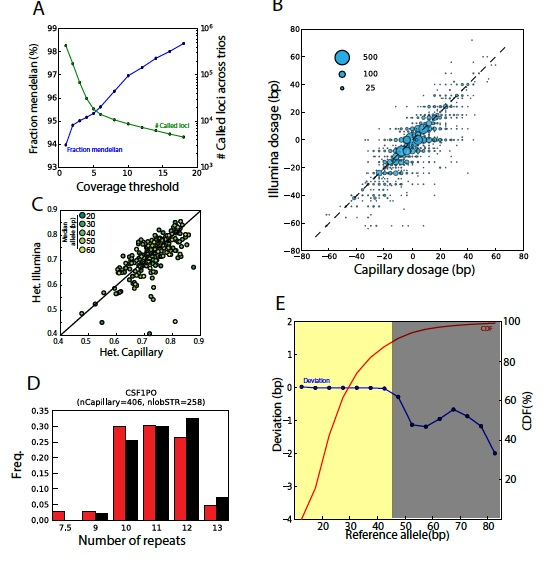
\includegraphics[width=0.5\textwidth]{Figures/Chapter3/Fig2.jpg}
\caption{\textbf{Quality assessments of the STR catalog} \textbf{(A) Consistency of lobSTR calls with Mendelian inheritance.} The blue line denotes the fraction of STR loci that followed Mendelian inheritance as a function of the read coverage threshold. The green line denotes the total number of calls in the three trios that passed the coverage threshold \textbf{(B) Concordance between lobSTR and capillary electrophoresis genotypes.} The STR calls were taken from the highly polymorphic Marshfield panel. The dosage is reported as the sum of base pair differences from the NCBI reference. The area of each bubble is proportional to the number of calls of the dosage combination and the broken line indicates the diagonal \textbf{(C) Comparison of heterozygosity rates for Marshfield panel STRs.} The color denotes the length of the median allele of the STR (dark-short; bright-long) \textbf{(D) A comparison of allelic spectra obtained by lobSTR and capillary electrophoresis for a CODIS marker in European individuals.} Red: lobSTR, black: capillary electrophoresis. nlobSTR and nCapillary indicate the number of alleles called in the respective call sets. \textbf{(E) The reliable range of lobSTR allelic spectra.} The figure presents the median deviation of the lobSTR calls from the NCBI reference as a function of the NCBI reference alleles (blue curve). Negative deviations indicate a potential preference towards ascertaining shorter alleles. STRs with reference alleles of up to $\sim$45bp show very minimal deviations (yellow region) and are expected to display unbiased frequency spectra with the current read lengths. These STR loci comprise close to 90\% of the total genotyped STRs in our catalog (red curve).}
\end{figure}

\subsection{Validation using population genetics trends}
To further assess the utility of our catalog, we tested its ability to replicate known population genetics trends. We specifically wondered about the quality of the most variable STR loci in the catalog. One hypothesis is that these loci are just extreme cases of genotyping errors; an alternative hypothesis is that these loci are truly polymorphic and can provide useful observations about the underlying populations.  We first compared the heterozygosities of the 10\% most variable autosomal loci across ten different subpopulations from Africa, East Asia, and Europe. Consistent with the Out-of-Africa bottleneck \cite{StonekingKrause2011}, we found that the genetic diversity of the African subpopulations significantly exceeded those of Europe and East Asia (sign test; $p < 10^{-50}$ for any African non-African pair) (\textbf{Figure \ref{fig:catfig3}a; \cite{SuppWillemsGymrekHighnamEtAl2014}}). Second, we focused on the 100 most heterozygous autosomal loci in our catalog and inspected the ability of STRUCTURE \cite{PritchardStephensDonnelly2000} to cluster a subset of the samples into three main ancestries in an unsupervised manner. Our results show that all of these samples clustered distinctly by geographical region (\textbf{Figure \ref{fig:catfig3}b}). These analyses demonstrate that even the most variable loci in the catalog still convey valid genetic information that can be useful for population genetic analyses. Finally, we also analyzed the genetic variability of all STRs with MAF$>$1\% on the autosome, X chromosome, and Y chromosome (\textbf{Figure \ref{fig:catfig3}c}). Autosomal STRs showed the highest variability, followed by STRs on the X and the Y chromosomes. This result is consistent with the differences in the effective population sizes of these three types of chromosomes, providing an additional sanity check.  

\begin{figure}[h!]
\centering
\label{fig:catfig3}
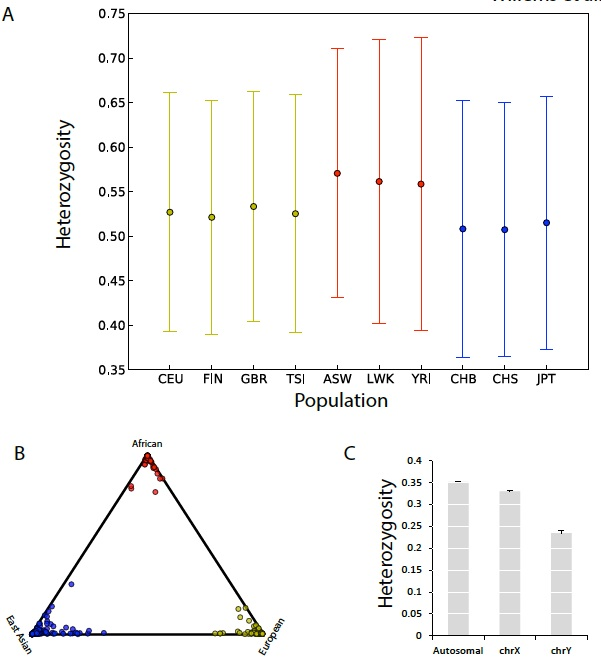
\includegraphics[width=0.5\textwidth]{Figures/Chapter3/Fig3.jpg}
\caption{\textbf{Evaluation of the STR catalog for population genetics} \textbf{(A) Genetic diversity of the 10\% most heterozygous autosomal loci in different populations.} Yellow: European, Red: African, Blue: East Asian. The mean heterozygosities (dot) of the African subpopulations consistently exceed those of the non-African subpopulations. The whiskers extend to ± one standard deviation. See Supplemental Table 3 for population abbreviations \textbf{(B) STRUCTURE clustering based on the 100 most polymorphic autosomal STR loci.} Each subpopulation clusters tightly by geographic origin. Color labels as in \textbf{(A). (C) Average STR heterozygosity as a function of chromosome type.} Bars denote the standard error.}
\end{figure}

In summary, the multiple lines of quality assessment suggest that our catalog can be used to infer patterns of human STR variations such as heterozygosity, allelic spectra, and population structure. The most notable shortcoming of the catalog is allelic dropouts stemming from the low sequencing coverage of the 1000 Genomes. However, the experiments above suggest that valuable summary statistics can be extracted from the call set despite this caveat. 

\subsection{Patterns of STR variation}
Despite a plethora of STR studies, there is no consensus in the literature regarding the effect of motif characteristics on STR variability. The classical study by Weber and Wong \cite{WeberWong1993} originally suggested that tetranucleotide STRs mutate more rapidly than those with dinucleotide motifs based on the analysis of de-novo mutation in trios for 50 STRs. This finding was recently supported by a much larger trio-based study of nearly 2500 STRs \cite{SunHelgasonMassonEtAl2012}. However, various other studies have suggested that dinucleotides have higher mutation rates \cite{ChakrabortyKimmelStiversEtAl1997,PembertonSandefurJakobssonEtAl2009}. These disagreements may largely stem from the fact that many of these studies considered very small panels of STRs that are subject to ascertainment biases. 

\begin{figure}[h!]
\centering
\label{fig:catfig4}
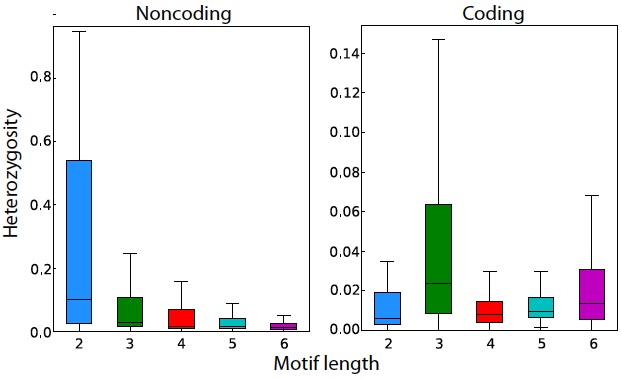
\includegraphics[width=0.5\textwidth]{Figures/Chapter3/Fig4.jpg}
\caption{\textbf{Motif length and coding capabilities as determinants of STR variability.} STR heterozygosity monotonically decreases with motif length for noncoding loci and is generally reduced in non-coding (left) versus coding regions (right). The box extends from the lower to upper quartiles of the heterozygosity distribution and the interior line indicates the median. The whiskers extend to the most extreme points within 1.5*IQR of the quartiles.}
\end{figure}

To address this open question, we analyzed the sequence determinants of STR variation in our catalog. We found that for noncoding STRs, variability monotonically decreased with motif length (\textbf{Figure \ref{fig:catfig4}}). In contrast, loci with trimeric and hexameric motifs were the most polymorphic among coding STRs. These STR loci can vary without introducing frameshift mutations and therefore may be exposed to weaker purifying selection. In addition, coding STRs demonstrated significantly reduced heterozygosity compared to noncoding STRs for periods 2-5bp (Mann-Whitney U test; $p < 0.01$, \cite{SuppWillemsGymrekHighnamEtAl2014}) while hexameric STRs showed no statistically significant difference in variability between these two classes. To ensure that the dependence between motif length and heterozygosity was not confounded by length or purity biases, we stratified STR heterozygosity for pure STRs based on major allele length and motif length. This analysis still showed an inverse correlation between motif length and STR variability after stratification based on the length of the most common allele \cite{SuppWillemsGymrekHighnamEtAl2014}. In addition, this analysis showed a monotonic increase in STR variability as a function of the major allele length. Similar trends also applied for STRs with various levels of impurities, albeit with a reduced magnitude of effect and slight deviations from monotonicity \cite{SuppWillemsGymrekHighnamEtAl2014}. This observation is concordant with previous studies \cite{Ellegren2000,LaiSun2003,WhittakerHarbordBoxallEtAl2003}.

Next, we explored the effect of nucleotide composition on STR variability, another issue for which the literature has not yet reached a consensus. Previous studies have suggested that AT repeats are the least variable motif for dinucleotide STRs \cite{PembertonSandefurJakobssonEtAl2009,BachtrogAgisImhofEtAl2000}, whereas other studies claimed that AT repeats are the most variable motif \cite{SunHelgasonMassonEtAl2012,KelkarTyekuchevaChiaromonteEtAl2008}. We repeated our analysis by stratifying the STRs based on motif sequence and major allele length \cite{SuppWillemsGymrekHighnamEtAl2014}. The resulting per-motif variability results were remarkably similar with those generated using a comparison of orthologous STRs in humans and chimps \cite{KelkarTyekuchevaChiaromonteEtAl2008}. Our analysis shows that AT repeats are in general more variable that AC repeats after controlling for length of the most major allele. Similarly, for most motif lengths, STRs with an [A]nT motif tend to be more variable with long major allele lengths. However, we could not find a clear pattern across motif lengths, which is similar to the result of a previous analysis of a few dozens Y-STRs \cite{BallantyneGoedbloedFangEtAl2010}. 

\subsection{The prototypical STR}
We also wondered about the prototypical pattern of variation of an STR locus in terms of the number of alleles and their distribution. We found that 30\% of STRs have a common polymorphism with at least two alleles with frequencies above 5\%. Dinucleotide STRs have the highest rate, with 48\% of these loci displaying a common polymorphism. Moreover, 30\% of all dinucleotide STRs have more than 3 alleles with a frequency above 5\%. On the other hand, hexanucleotide STRs have the lowest common polymorphism rate, with only 13\% of these loci displaying a common polymorphism \cite{SuppWillemsGymrekHighnamEtAl2014}.  

Next, we turned to finding the prototypal allelic spectra of STRs. For each STR, we normalized the reported alleles such that they reflected the distance in number of repeats from the locus' most common allele. Then, we generated histograms that show the allelic spectra by aggregating all the alleles of STRs with the same motif length. This coarse-grained picture was similar across repeat lengths \cite{SuppWillemsGymrekHighnamEtAl2014}.  The allelic spectrum of an STR is unimodal and relatively symmetric. There is one, highly prevalent major allele, two less common alleles one repeat above and one repeat below the most common allele, and a range of rare alleles with monotonically decreasing frequency that reach over ±5 repeats from the most common allele.  

We also wondered about the population differentiation of autosomal STRs. We analyzed the $R_{st}$ \cite{Slatkin1995} for each STR between African, Asian, and European populations for STRs with heterozygosity above 5\% \cite{SuppWillemsGymrekHighnamEtAl2014}. The average Rst was between 4.5-6\% across the motif lengths and the median was around 2-3\%. In coding regions, when compared to noncoding STRs, the average $R_{st}$ was less than half for trimeric STRs but the same for hexameric STRs. Our results regarding population differentiation using STRs are reminiscent of a classical study that found similar levels of differentiation by analyzing close to 800 STR markers \cite{RosenbergPritchardWeberEtAl2002}.

\subsection{STRs in the NCBI reference and LoF analysis}
We were interested in assessing how well the most common alleles are represented in the NCBI reference (\textbf{Figure \ref{fig:catfig5}a}). We found that for over 69,000 loci (10\% of our reference set), the most common allele across the 1000 Genomes populations was at least one repeat away from the NCBI hg19 reference allele. Furthermore, the length of the most common allele only matched the length of the orthologous chimp STR 50\% of the time, reflecting the high mutability of these loci. In addition, 15,581 loci (2.25\%) in the reference genome were 10bp or more away from the most common allele in our dataset.  

For STRs in coding regions, the most common allele for 48 loci (1.1\% of coding STRs) did not match the allele present in the NCBI reference \cite{SuppWillemsGymrekHighnamEtAl2014}. In 46 out of 48 of these cases, these differences occurred for loci with trinucleotide or hexanucleotide repeats and conserved the reading frame. Moreover, for the two loci whose most common alleles were frame-shifted, these variations are unlikely to trigger the non-sense mediated decay pathway. The deletion of one 4bp unit in \emph{DCHS2} occurs a few nucleotides before the annotated RefSeq stop codon. This variation slightly alters the location of the stop codon and affects only five amino acids in the C-terminus of the protein. The 14bp deletion in \emph{ANKLE1} occurs in the last exon of the gene and introduces about 20 new amino acids into the tail of the protein. 

We also sought to identify a confident set of STR loci with relatively common loss of function (LoF) alleles. To accomplish this goal, we considered only alleles supported by at least two reads and 30\% of the total reads per called genotype. We further required that alleles be carried by 10 or more samples. Seven common LoF alleles across five genes passed this criterion: \emph{DCHS2, FAM166B, GP6, SLC9A8}, and \emph{TMEM254} \cite{SuppWillemsGymrekHighnamEtAl2014}. Out of these 5 genes, only \emph{GP6} has known implications for a Mendelian condition: a mild platelet-type bleeding disorder \cite{DumontLasneRothschildEtAl2009,HermansWittevrongelThysEtAl2009}. However, the LoF mutation in this gene resides in the last exon and is unlikely to induce the non-sense mediated decay pathway. In conclusion, the LoF analysis indicates that common STR polymorphisms rarely disrupt the reading frame.  

\subsection{Linkage disequilibrium between STRs and SNPs}
The linkage disequilibrium (LD) structure of STRs and SNPs is largely unknown. On top of recombination events, the SNP-STR LD structure also absorbs STR back mutations that could further shift these pairs of loci towards equilibrium. However, there is minimal empirical data in the literature about the pattern of this LD structure, most of which pertains to a few hundred autosomal Marshfield markers \cite{PayseurPlaceWeber2008}. To get a chromosome-wide estimate, we inspected STR loci on the hemizygous X chromosomes in male samples. Similar to the Y chromosome data, these calls do not suffer from allelic dropouts and are already phased with SNP alleles, conferring a technically reliable dataset for a chromosome-wide analysis.  

\begin{figure}[h!]
\centering
\label{fig:catfig5}
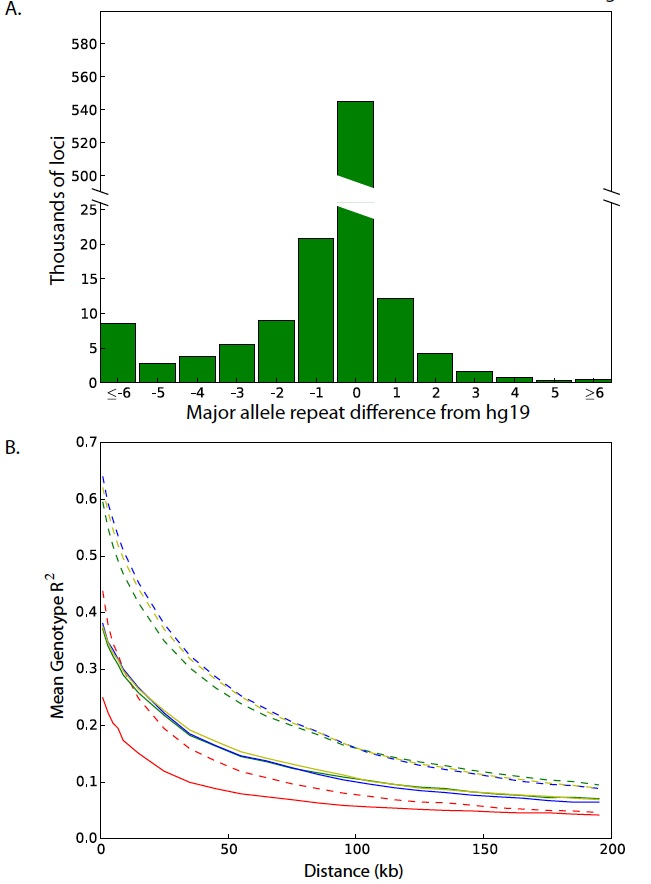
\includegraphics[width=0.5\textwidth]{Figures/Chapter3/Fig5.jpg}
\caption{\textbf{Population-scale analyses of STR variation (A) Distribution of base-pair differences between each locus' most common allele and the NCBI reference allele (B) Patterns of linkage disequilibrium for SNPs and STRs on the X chromosome.} SNP-SNP LD (dashed lines) generally exceeds SNP-STR LD (solid lines) across a range of distances and for Africans (red), Admixed Americans (green), Europeans (yellow) and East Asians (blue).}
\end{figure}

We determined the LD in terms of the $R^2$ between SNPs and STRs as a function of the distance between these markers. Only STRs and SNPs with common polymorphisms were used for the analysis. Hexameric STRs were not included due to the small sample size of 24 sites; for the other repeat motifs, we obtained hundreds to thousands of polymorphic markers. We stratified the STR-SNP LD based on the four major continental populations (Africa, Asia, Europe, and America) and contrasted them to the patterns for classical SNP-SNP LD (\textbf{Figure \ref{fig:catfig5}b}). In all cases, the SNP-SNP LD consistently exceeded mean STR-SNP LD. In addition, the African population demonstrated markedly reduced levels of SNP-STR LD and SNP-SNP LD, consistent with its larger effective population size. In general, dinucleotide STRs showed the weakest LD with nearby SNPs, which likely stems from their higher mutation rates \cite{SuppWillemsGymrekHighnamEtAl2014}. To ensure that the reduction in STR-SNP LD did not stem from comparing $R^2$ values for multiallelic and biallelic makers, we converted the STR alleles to binary markers, where the two states corresponded to the most common allele and all alternative alleles grouped together. The resulting levels of mean SNP-STR LD using these binary genotypes were nearly identical to those obtained using the multiallelic STR genotypes, indicating that this potential issue had little effect \cite{SuppWillemsGymrekHighnamEtAl2014}. 

Overall, this analysis shows that the average SNP-STR LD is approximately half of the SNP-SNP LD for variations with the same distance on the X chromosome. Since the effective population size of the X chromosome is smaller than that of the autosome, the STR-SNP LD should be even smaller on the autosome. These results suggest that association studies with tagging SNPs might be considerably underpowered to detect loci with causal STRs, specifically dinucleotide loci. 

\section{Discussion}
In the last few years, population-scale sequencing projects have made tremendous progress in documenting genetic variation across human populations. The 1000 Genomes Project has already reported approximately 40 million SNPs, 1.4 million insertion and deletions, and over 10,000 structural variants \cite{AbecasisAltshulerAutonEtAl2010} . Similar catalogs, albeit to lesser degrees of completeness, have been produced for other types of variations, such as LINE-1 insertions \cite{EwingKazazian2011} and Alu repeat variations \cite{HormozdiariAlkanVenturaEtAl2011}. Here, we presented a population-scale analysis of STR variation, adding another layer of genetic variation to existing catalogs.  

Our analysis significantly augments the level of knowledge of STR variation. Currently, dbSNP reports data for only 5,500 STR loci. Our catalog provides data on close to 700,000 STR loci, which encompasses 97\% of the STRs with motifs of 2-6bp in the genome, and contains over 300,000 STR loci with a MAF of over 1\%. One caveat of our catalog is the low reliability of individual genotypes due to allelic dropout. Nonetheless, we showed using multiple lines of analysis that summary statistic results such as frequency spectra and variation trends can be extracted from the catalog for most of the STRs. Another caveat of our catalog is that with the mixture of 76bp and 100bp sequencing reads, we could only unbiasedly ascertain the allelic spectra of about 90\% of the STRs, those with NCBI alleles of up to 45bp. To indicate this caveat, our website alerts users about a potential bias in the allelic spectrum when inspecting STRs with reference allele length beyond this range. However, we expect caveat will be alleviated in the near future with the public release of the Phase 3 data that re-sequenced a large number of Phase 1 samples with 100bp Illumina reads. We expect that this dataset will enable the generation of unbiased allelic spectra for longer STRs. 

Despite these limitations, our data provides several biological insights about STR variation. Shorter repeat motif, longer major allele, higher purity of the repeat motif, and residing outside of a coding region are all associated with an increase in STR variability. Most of the STR loci display a unimodal distribution with one very common allele and series of minor alleles with rapidly declining frequencies. This picture suggests that the stepwise mutation model largely describes the creation of new alleles in most of these loci. An open question is the exact mutation rate per generation for each locus in the genome. This question is theoretically addressable with sufficiently large number of samples by analyzing the distribution of squared differences in the repeat size between two alleles of the same locus \cite{SunHelgasonMassonEtAl2012}. However, this question cannot be addressed by our call set due to the large number of allelic dropouts that might confound such an analysis and should be addressed with datasets obtained from deeply covered genomes. 

The landscape of STR variations in the apparently healthy 1000 Genomes individuals suggests several rules of thumbs for analyzing STR variations for medical sequencing. Previous work found that membrane proteins of several pathogens contain STR loci with non-triplet motifs whose variations can be beneficial to the organism \cite{GemayelVincesLegendreEtAl2010}. These STRs confer high evolvability and adaptability of these proteins by dynamically changing the reading frame. In contrast, our data suggests that for the vast majority of human proteins, frame-shift mutations in their STR regions are not favorable. Only a handful of STRs harbor common frame-shift polymorphisms and half of the LoF alleles create a very small change in the C-terminus tail of the protein. Based on these observations, we hypothesize that most of the non-triplet coding STRs are not well tolerated and are exposed to negative selection similar to regular indels in the same region. Therefore, it is advisable for medical sequencing projects to also analyze these loci and treat them as regular LoF alleles rather than filtering them. This rule of thumb is well-echoed in a recent study of medullary cystic kidney disease type 1 that implicated the genetic pathology in a frame-shift mutation caused by a length change of a homopolymer run \cite(Kirby et al. 2013). For in-frame STR variations, our call set contains deep allelic spectra of most of these loci, providing reference distributions of apparently healthy alleles. These spectra can be used to identify atypical STR alleles and might serve as an indicator for pathogenicity.  

Although STR alleles within our call set rarely induced frame-shifts, they may introduce premature stop codons by modulating the splicing machinery. Several prior studies have observed a direct dependence of splicing efficiency on STR repeat number for \emph{CFTR} \cite{HefferonGromanYurkEtAl2004}, \emph{HTT} \cite{SathasivamNeuederGipsonEtAl2013} and \emph{NOS3} \cite{HuiStanglLaneEtAl2003}. To facilitate the analysis of such cases, we created a dedicated table on the catalog website that specifies all of the 2,237 STRs that reside within 20 base pairs of an exon-intron boundary.  

Another issue raised by our findings is the potential contribution of STRs to complex traits. Using the prototypical allelic spectra, we estimate that the average variance of STR repeat dosage is 3, 0.7, 0.4, 0.25 and 0.1 for 2-6mer STRs, respectively. Interestingly, the theoretical maximum variance for a bi-allelic SNP dosage is 0.5, six times smaller than the observed variance of dinucleotide STRs. From a theoretical statistical genetics perspective, this suggests that causal dinucleotide STR loci could explain a considerable fraction of phenotypic variance even with a relatively modest effect size. Therefore, if each STR allele in a locus slightly changes a quantitative trait in a gradual manner, the net effect on the phenotypic variance could be quite large due to the wide range of these alleles and their relatively high frequencies. Interestingly, we found that loci with dinucleotide motifs show relatively weak LD with SNPs, suggesting that GWAS studies with SNP arrays are prone to miss causal STR loci. Given the theoretical potential of STRs to contribute to phenotypic variance on one hand and their weaker LD to tagging SNPs on the other hand, one intriguing possibility is that STRs contribute to the missing heritability phenomenon of complex traits \cite{ManolioCollinsCoxEtAl2009,PressCarlsonQueitsch2014}. Our hope is that this catalog can be a reference point to test this hypothesis in future studies.  

\section{Methods}
\label{sec:catmet}

\subsection{Call set generation}
The raw sequencing files for Phase 1 of the 1000 Genomes Project were analyzed.

The lobSTR calls were generated using computing resources hosted by Amazon Web Services, GitHub version 8a6aeb9 of the lobSTR genotyper and Github version a85bb7f of the lobSTR allelotyper (\url{https://github.com/mgymrek/lobstr-code}). In particular, the lobSTR genotyper was run using the options fft-window-size=16, fft-window-step=4 and bwaq=15 and a default minimum flanking region of 8bp on both sizes of the STR region. Reads that were aligned to multiple locations were excluded from the analysis. PCR duplicates were removed from the resulting BAM files for each experiment using SAMtools \cite{LiHandsakerWysokerEtAl2009}. The individual BAMs were merged by population and the lobSTR allelotyper was run using all population BAMs concurrently, the include-flank option and version 2.0.3 of lobSTR's Illumina PCR stutter model.  

RepeatSeq (available \url{http://github.com/adaptivegenome/repeatseq}) was run using default parameters on the read alignments produced by the 1000 Genomes project. 

For both programs, we used the set of 700,000 STRs that was constructed using the second-order Markov framework \cite{SuppWillemsGymrekHighnamEtAl2014}. 

\subsection{Estimating the number of samples per locus and number of loci per sample}
The distributions of the call set parameters were smoothed using the gaussian\_kde function in the scipy.stats python package. Covariance factors of 0.01 and 0.025 were used to smooth the samples per locus and loci per sample distributions, respectively. 

\subsection{Saturation analysis}
We determined the number of loci with calls for sample subsets containing 1, 5, 10, 25, 50, 100, 250, 500, 750 and 1000 individuals. In particular, we began by randomly selecting 1 individual. To create a subset of 5 individuals, we then added 4 more random individuals and so on. For each of these sample subsets, we determined the number of loci with one or more STR calls across all samples in the subset. We repeated this whole process 10 times and used the median number of called loci across each of the 10 repetitions to create the saturation profile for all loci. 

We also determined whether loci had a MAF $>$ 1\% using all 1009 samples. We then used a procedure analogous to the one described above to select subsets of samples and determine whether or not each of these loci had a corresponding call in each subset. This procedure resulted in the saturation profile for loci with MAF $>$ 1\%. 

\subsection{Mendelian inheritance}
The three low-coverage trios contained within the dataset consisted of the following sample sets: HG00656, HG00657, HG00702 (trio 1), NA19661, NA19660, NA19685 (trio 2) and NA19679, NA19678, NA19675 (trio 3). To assess the consistency with Mendelian inheritance for a given trio, only loci for which all three samples had calls were analyzed. The coverage assigned to each trio of calls corresponded to the minimum coverage across the three samples. 

\subsection{Capillary electrophoresis comparison}
Capillary electrophoresis comparison Marshfield genotypes \cite{Rosenberg2006} were downloaded from \url{http://www.stanford.edu/group/rosenberglab/data/rosenbergEtAl2005/combined-1048.stru}. Prior to comparing genotypes, offsets were calculated to match the lobSTR calls to the length of the Marshfield PCR products. For each locus, all observed offsets were considered and scored and the optimally scoring offset across all samples was selected. In particular, for each sample, an offset was scored as a 1, 0.5, 0.25 or 0 if the lobSTR calls matched exactly, were homozygous and recovered one Marshfield allele, were heterozygous and recovered one Marshfield allele or did not match at all, respectively.  Only loci with at least 20 calls were considered in the comparison. Finally, the Pearson correlation coefficient was calculated using the sum of the allele length differences from hg19 for each locus in each sample.

Y-chromosome PowerPlex genotypes were downloaded from the 1000 Genomes Y chromosome working group FTP site. Offsets were once again calculated to match the length of the PCR products to the lobSTR calls. For each locus, the offset was calculated as the most common difference between the lobSTR and PowerPlex genotypes across samples. Only loci with at least 5 calls were considered in the comparison and the R2 was calculated between the allele length differences from hg19 for each locus in each sample. In addition, the 15 heterozygous lobSTR calls were ignored.  

Slopes and $R^2$ values for STR dosage comparisons were calculated using the linregress function in the scipy.stats package.  To mitigate the effects of outliers, we explored using regular linear regression, regression with a zero intercept and L1 penalized regression. The resulting slopes were essentially invariant to the calculation method and so statistics were reported based on traditional linear regression.  

\subsection{Heterozygosity calculations}
For each analysis, heterozygosity was calculated using the aggregated frequency spectra according to the formula $H_E = 1-\sum_i f_i^2$ where $f_i$ denotes the frequency of the $i$th allele at the locus.

\subsection{Summary statistic comparisons}
The allelic spectra of the Marshfield panel were downloaded from \url{http://research.marshfieldclinic.org/genetics/genotypingData_Statistics/markers/} and parsed using a custom Perl script (data and script available on \url{https://github.com/erlichya/str_catalog_supplemental_scripts}). Samples from the CEU, GBR, TSI, and FIN subpopulations were analyzed, and only markers with more than 50 calls were included.

We utilized all of the lobSTR calls for the CEU, GBR and FIN subpopulations to generate the lobSTR frequency spectra for each CODIS marker. Spectra were not available for 3 of the CODIS markers (D21S11, VWa, TPOX). D21S11 is too long to be spanned by Illumina reads; we had annotation difficulties for VWa and TPOX (assigning the correct STR in hg19 to the NIST STR). We then compared the available frequency spectra to those published for a Caucasian population in the United States \cite{BudowleSheaNiezgodaEtAl2001} . Because of some annotation differences between the capillary data and our reference locations, we shifted the lobSTR spectra for the D8S1179 marker by +2 repeat units. Finally, repeat lengths for which the maximum frequency was less than 2\% were not displayed. 

\subsection{Comparison of population heterozygosity}
To obtain accurate measures of heterozygosity, autosomal STR loci with less than 30 calls in any of the 10 subpopulations considered were ignored. Of the remaining loci, the 10\% most heterozygous (24,637 loci) were selected and their means and standard deviations were calculated. To determine whether a pair of populations had systematically different heterozygosity at these loci, we paired the heterozygosities for each locus and counted the number of pairs in which population A had a larger heterozygosity than population B. Ignoring the relatively small number of loci in which heterozygosities were identical, the p-value for this over/underrepresentation was then calculated using the cdf function in the scipy.stats.binom python package.  

\subsection{Deviation of lobSTR calls from the NCBI reference}
For each locus with one or more genotyped samples, we calculated the mean deviation of all samples' genotypes from the NCBI reference allele. We then pooled these per-locus deviations by reference allele length using 5bp intervals. The median within each length bin resulted in the corresponding plot of deviation vs. reference allele length. 

\subsection{Sample clustering}
STRUCTURE version 2.3.4 was utilized to perform the MCMC-based clustering. The program was run using MAXPOPS=3, BURNIN=500000, NUMREPS=1000000, no prior population information, unphased genotypes, the admixture model and no linkage disequilibrium. All 321 samples from the JPT, CHB, YRI and CEU subpopulations present in the data were clustered based on the 100 most heterozygous autosomal STRs with at least 750 called samples. Samples for which at least 75\% of the selected makers were missing calls were not including in the resulting visualization. The final triangle plot therefore contained data for 71, 80, 81, and 82 samples from the CEU, CHB, JPT and YRI populations, respectively.  

\subsection{STR variability trends}
Analysis was restricted to STRs with at least 100 called samples. STRs that overlapped an annotated RefSeq translated region were regarded as coding and these annotations were downloaded from the UCSC table browser on 2/11/2014.  The mannwhitneyu function in the scipy.stats python package was used to test for significant differences between coding and non-coding STR heterozygosity. For analyses related to allele length or purity, STRs were further restricted to those whose most common allele matched the hg19 reference to enable calculation of the locus' purity. In particular, the purity of each of these STRs was calculated as the fraction of possible positions within the STR region where the subsequent bases corresponded to a cyclic permutation of the STR's motif. The pearsonr function in the scipy.stats python package was used to calculate the Pearson correlation coefficients and their associated p-values, where each STR's length and heterozygosity represented an individual point. Finally, to generate the plots of heterozygosity vs. length, the heterozygosity for each length was calculated as the mean variability of loci within 2bp.   

\subsection{Extraction of orthologous chimp STR lengths}
Tandem Repeats Finder was run on the panTro4 assembly of the chimp genome using the default parameters and a minimum score threshold of 5. To resolve overlapping repeats, we discarded repeats with period greater than six and scanned from low to high coordinates and selected the highest scoring repeat for each overlap conflict. The chimp coordinates were mapped to hg19 coordinates using liftOver and a minimum mapping fraction of 50\%. We then intersected these coordinates with those of our reference panel and retained those loci within our panel that had a single intersecting chimp repeat whose motif matched. This resulted in orthologous chimp repeats for $\sim$83\% of our reference set of STRs.  

\subsection{$R_{ST}$ levels}
The Rst was calculated according to Slatkin \cite{Slatkin1995} using a custom Python script (code available on \url{https://github.com/erlichya/str_catalog_supplemental_scripts}). The African, European and Asian populations were comprised of the same subpopulations used throughout this study, except that the ASW population was omitted due to potential admixture. Only loci with heterozygosity above 5\% and at least 100 genotyped samples were considered. 

\subsection{Assessing linkage disequilibrium}
In order to avoid phasing SNPs and STRs, we only analyzed X chromosome genotypes in male samples. SNP calls for the corresponding samples were obtained from the 1000 Genomes Phase 1 11/23/2010 release and any pseudoautosomal loci were ignored. Analysis of STR-SNP LD was restricted to STR loci with both a heterozygosity of at least 9.5\% and at least 20 genotypes for each super population (African, East Asian, European and Ad Mixed American). For each STR that met this requirement, we identified all SNPs within 200 KB of the STR start coordinate. After filtering out SNPs with a MAF below 5\% in any of the four super populations, we calculated the level of LD for the remaining STR-SNP pairs. In particular, the $R^2$ was calculated between the SNP genotype indicator variable and the base pair difference of the STR from the reference. We also recalculated the STR-SNP LD after converting the STR alleles to binary variables, where the most common allele and all alternative alleles were mapped to 0 and 1, respectively. This binary mapping was applied to each super population individually. 

For SNP-SNP LD calculations, a seed SNP was identified for each STR meeting the aforementioned requirements. In particular, the SNP closest to the STR’s start coordinate with MAF $>$ 5\% for each super population was selected. If no such SNP existed within 1Kb, no SNP was selected and the STR was omitted from the STR-SNP LD analysis. Otherwise, we identified all SNPs within 200 KB of the seed SNP and once again removed SNPs with a MAF $<$ 5\% in any of the super populations. The LD between the seed SNP and each of these remaining SNPs was then assessed as the R2 between the two SNP genotype indicator variables.  

\section{Acknowledgements}
M.G. is supported by the National Defense Science and Engineering Graduate Fellowship. Y.E. is an Andria and Paul Heafy Family Fellow and holds a Career Award at the Scientific Interface from the Burroughs Wellcome Fund. This study was funded by a gift from Cathy and Jim Stone and an AWS Education Grant award. The authors thank Chris Taylor Smith, Wei Wei, Qasim Ayub, and Yali Xue for providing the results of the Y-STR panel for the 1000 Genomes individuals and the 1000 Genomes Project members for useful discussions. Y.E. dedicates this manuscript to Lia Erlich that was born during the last revision of this work.
\iffalse \bibliography{MGymrekRefs.bib} \fi

\chapter{Abundant contribution of short tandem repeats to gene expression variation in humans}

\hzline

Most of this chapter was first published as:

\begin{itemize}
\item[] \textbf{Gymrek M}, Willems TF, Guilmatre A, Zeng H, Markus B, Georgiev S, Daly MJ, Price AL, Pritchard JK, Sharp AJ, Erlich Y. Abundant contribution of short tandem repeats to gene expression ariation in humans. \emph{Nature Genetics}. (2015).
\end{itemize}

\hzline

\textbf{Abstract:} The contribution of repetitive elements to quantitative human traits is largely unknown. Here, we report a genome-wide survey of the contribution of Short Tandem Repeats (STRs), one of the most polymorphic and abundant repeat classes, to gene expression in humans. Our survey identified 2,060 significant expression STRs (eSTRs). These eSTRs were replicable in orthogonal populations and expression assays. We used variance partitioning to disentangle the contribution of eSTRs from linked SNPs and indels and found that eSTRs contribute 10\%-15\% of the cis-heritability mediated by all common variants. Further functional genomic analyses showed that eSTRs are enriched in conserved regions, co-localize with regulatory elements, and can modulate certain histone modifications. By analyzing known GWAS hits and searching for new associations in 1,685 deeply-phenotyped whole-genomes, we found that eSTRs are enriched in various clinically-relevant conditions. These results highlight the contribution of short tandem repeats to the genetic architecture of quantitative human traits.

\section{Introduction}
In recent years, there has been tremendous progress in identifying genetic variants that affect expression of nearby genes, termed cis expression quantitative trait loci (cis-eQTLs). Multiple studies have shown that disease-associated variants often overlap cis-eQTLs in the affected tissue \cite{MoffattKabeschLiangEtAl2007,BarrettHansoulNicolaeEtAl2008,ArdlieDelucaSegreEtAl2015}. These observations suggest that understanding the genetic architecture of the transcriptome may provide insights into the cellular-level mediators underlying complex traits \cite{NicaMontgomeryDimasEtAl2010,NicolaeGamazonZhangEtAl2010,WardKellis2012}. So far, eQTL-mapping studies have mainly focused on SNPs and to a lesser extent on bi-allelic indels and CNVs as determinants of gene expression \cite{StrangerNicaForrestEtAl2007,GrundbergSmallHedmanEtAl2012,LappalainenSammethFriedlanderEtAl2013}. However, these variants do not account for all of the heritability of gene expression attributable to cis-regulatory elements as measured by twin studies, leaving on average about 20-30\% unexplained \cite{GrundbergSmallHedmanEtAl2012,WrightSullivanBrooksEtAl2014}.  It has been speculated that such heritability gaps could indicate the involvement of repetitive elements that are not well tagged by common SNPs \cite{ManolioCollinsCoxEtAl2009,PressCarlsonQueitsch2014}. 

To augment the repertoire of eQTL classes, we focused on Short Tandem Repeats (STRs), one of the most polymorphic and abundant types of repetitive elements in the human genome \cite{Ellegren2004,GemayelVincesLegendreEtAl2010}. These loci consist of periodic DNA motifs of 2-6bp spanning a median length of around 25bp. There are about 700,000 STR loci covering almost 1\% of the human genome. Their repetitive structure induces DNA-polymerase slippage events that add or delete repeat units, creating mutation rates that are orders of magnitude higher than those of most other variant types \cite{WeberWong1993,Ellegren2004}. Over 40 Mendelian disorders, such as Huntington’s Disease, are attributed to STR mutations, most of which are caused by large expansions of trinucleotide coding repeats \cite{Mirkin2007}. 

Several properties of STRs suggest they may play a regulatory role. In vitro studies have shown that STR variations can modulate the binding of transcription factors \cite{ContenteDittmerKochEtAl2002,MartinMakepeaceHillEtAl2005}, change the distance between promoter elements \cite{WillemsPaulHeideEtAl1990,YogevRosengartenWatson-McKownEtAl1991}, alter splicing efficiency \cite{HefferonGromanYurkEtAl2004,HuiHungHeinerEtAl2005}, and induce irregular DNA structures that may modulate transcription \cite{RothenburgKoch-NolteRichEtAl2001}. In vivo experiments have reported specific examples of STR variations that control gene expression across a wide range of taxa, including Haemophilus influenza \cite{WeiserLoveMoxon1989}, Saccharomyces cerevisiae \cite{VincesLegendreCaldaraEtAl2009}, Arabidopsis thaliana \cite{SureshkumarTodescoSchneebergerEtAl2009}, and vole \cite{HammockYoung2005}. Recent studies reported that dinucleotide repeats are a hallmark of enhancers in Drosophila and are enriched in predicted enhancers in humans \cite{Yanez-CunaArnoldStampfelEtAl2014}. Human promoters also disproportionately harbor STRs \cite{SawayaBagshawBuschiazzoEtAl2013} and the presence of STRs in promoters or transcribed regions greatly increases the divergence of gene expression profiles across great apes \cite{SonayCarvalhoRobinsonEtAl2015}, suggesting that STRs play a key role in the evolution of expression. Several candidate-gene studies in human indeed reported that STR variations modulate gene expression \cite{GebhardtZankerBrandt1999,ShimajiriArimaTanimotoEtAl1999,WarpehaXuLiuEtAl1999,ContenteDittmerKochEtAl2002,RockmanWray2002} and alternative splicing \cite{HuiStanglLaneEtAl2003,HefferonGromanYurkEtAl2004,SathasivamNeuederGipsonEtAl2013}. In one example, a recent study found that the underlying mechanism behind a GWAS signal for Ewing Sarcoma is a sequence variant in an AAGG repeat that increases the binding of the EWSR1-FLI1 oncoprotein resulting in EGF2 overexpression \cite{GrunewaldBernardGilardi-HebenstreitEtAl2015}. Despite these accumulating lines of evidence, there has been no systematic evaluation of the contribution of STRs to gene expression in humans. 

To this end, we conducted a genome-wide analysis of STRs that affect expression of nearby genes, termed expression STRs (eSTRs), in lymphoblastoid cell lines (LCLs), a central ex-vivo model for eQTL studies. Next, we used a multitude of statistical genetic and functional genomics analyses to show that hundreds of these eSTRs are predicted to be functional. Finally, we tested the involvement of eSTRs in clinically relevant phenotypes.

\chapter{Conclusion and future directions}
\label{chap:conc}
% TODO write this!

% lobSTR
% mention improvements, now uses bwa-mem
% mention hipstr, gatk, imputation

\subsubsection{Existing tools for genotyping STRs from sequencing data}
When we began this work, no dedicated tool for genotyping STRs from sequencing data existed. McIver \emph{et al.} \cite{McIverFondonSkinnerEtAl2011} evaluated STR variation in the 1000 Genomes Project \cite{AbecasisAltshulerAutonEtAl2010} samples. However their results were limited to the short variations that could be captured by aligners with poor indel sensitivity, and therefore vastly underestimated polymorphism levels. A major contribution of our work was develop the first efficient algorithm for generating accurate STR genotypes, called lobSTR \cite{GymrekGolanRossetEtAl2012} and described in \autoref{chap:lobstr}. Over the last several years, additional tools have arisen:

\begin{enumerate}
\item \textbf{STRViper} \cite{CaoTaskerWilladsenEtAl2014}: Uses insert size between paired end sequencing reads to detect STR variations.
\item \textbf{RepeatSeq} \cite{HighnamFranckMartinEtAl2013}: uses Bayesian model selection to genotype previously aligned STR-containing reads.
\item \textbf{STR-FM} \cite{FungtammasanAnandaHileEtAl2015}: uses a method based on lobSTR's algorithm but with a modified detection step for increased sensitivity of short repeats and may be applied to non-diploid samples.
\end{enumerate}

The first two tools operate on previously existing alignments, and so are limited by the quality of the upstream aligner. The third may provide improvements to STR calling, especially at homopolymers which are extremely noisy in sequencing data. So far, these tools have not seen widepsread use in mainstream sequence analysis.

In addition to STR-specific callers, a new class of variant callers, including GATK \cite{McKennaHannaBanksEtAl2010} HaplotypeCaller, Platypus \cite{RimmerPhanMathiesonEtAl2014}, and Scalpel \cite{NarzisiOextquotesingleRaweIossifovEtAl2014}, perform local reassembly of diploid haplotypes. These methods can theoretically genotype STRs quite accurately, albeit with greatly increased computational costs. There has so far been no systematic evaluation of their performance at STRs, but these tools may be promising for STR analysis in the future.

\subsection{Long-read technology can capture long repetitive regions}
A major limitation of analyzing STRs from high throughput sequencing data is the short read length. Only reads entirely spanning an STR are informative of the repeat length, and sufficient flanking region on either side of the STR is required for accurate alignment. While the mainstream sequencing technology from Illumina is limited to sequencing at most several hundred base pairs in a single read, alternative sequencing platforms, such as PacBio's SMRT (single molecule real time) sequencing \cite{EidFehrGrayEtAl2009} and the new Nanopore technology \cite{ClarkeWuJayasingheEtAl2009}, can now produce much longer read lengths of up to several thousand base pairs.

These technologies may be used to sequence long repeats observed in expansion disorders such as Fragile X \cite{LoomisEidPelusoEtAl2012} or ataxias \cite{DoiMonjoHoangEtAl2013}, and other complex regions of the genome. Chaisson \emph{et al} \cite{ChaissonHuddlestonDennisEtAl2015} recently applied SMRT to sequence a haploid genome to 40x coverage with an average read length of 5kb. With these long reads, they were able to close 50 gaps in the human genome reference assembly, which were highly enriched for short tandem repeats and other repeats embedded in larger, more complex tandem arrays of degenerate repeats. With longer and longer read lengths, we may soon be able to analyze STRs, as well as other repetitive elements such as variable number tandem repeats (VNTRs) and retrotransposons that were previously inaccessible using sequencing studies.
\appendix
\iffalse \bibliography{MGymrekRefs.bib} \fi

\chapter{Identifying personal genomes by surname inference}
\label{chap:surname}
\hzline

Most of this chapter was first published as:

\begin{itemize}

\item[] \textbf{Gymrek M}, McGuire A, Golan D, Halperin E, Erlich Y. Identifying personal genomes by surname inference. \emph{Science}. (2013).
\end{itemize}

\hzline


\textbf{Abstract:} Sharing sequencing datasets without identifiers has become a common practice in genomics. Here, we report that surnames can be recovered from personal genomes by profiling short tandem repeats on the Y-chromosome (Y-STRs) and querying recreational genetic genealogy databases. We show that a combination of a surname with other types of metadata, such as age and state, can be used to triangulate the identity of the target. A key feature of this technique is that it entirely relies on free, publicly accessible Internet resources. We quantitatively analyze the probability of identification for US males. We further demonstrate the feasibility of this technique by tracing back with high probability the identities of multiple participants in public sequencing projects.

\section{Main Text}
Surnames are paternally-inherited in most human societies, resulting in their co-segregation with Y-chromosome haplotypes \cite{SykesIrven2000,KingBallereauSchurerEtAl2006,McEvoyBradley2006,KingJobling2009,KingJobling2009a}. Based on this observation, multiple genetic genealogy companies offer services to reunite distant patrilineal relatives by genotyping a few dozen highly polymorphic short tandem repeats across the Y-chromosome (Y-STRs). The association between surnames and haplotypes can be confounded by non-paternity events, mutations, and adoption of the same surname by multiple founders \cite{KingJobling2009}. The genetic genealogy community addresses these barriers with massive databases that list the test results of Y-STR haplotypes along with their corresponding surnames. Currently, there are at least eight databases and numerous surname project websites that collectively contain hundreds of thousands surname-haplotype records (\textbf{Supplementary Table \ref{tab:sursuptab1}}). 

The ability of genetic genealogy databases to breach anonymity has been demonstrated in the past. In a number of public cases, male adoptees and descendants of anonymous sperm donors used recreational genetic genealogy services to genotype their Y-chromosome haplotypes and to search the companies' databases \cite{Lehmann-Haupt2010,Naik2009,Stein2005,Motluk2005}. The genetic matches identified distant patrilineal relatives and pointed to the potential surnames of their biological fathers. By combining other pieces of demographic information, such as date and place of birth, they fully exposed the identity of their biological fathers. Lunshof et al \cite{LunshofChadwickVorhausEtAl2008} was the first to speculate that this technique could expose the full identity of participants in sequencing projects. Gitschier \cite{Gitschier2009} empirically approached this hypothesis by testing 30 Y-STR haplotypes of CEU participants in these databases and reported that potential surnames can be detected.  [CEU participants are multigenerational familes of  northern and western European ancestry in Utah who had originally had their samples collected by CEPH (Centre d'Etude du Polymorphisme Humain) and were later reconsented to participate in the HapMap project.] However, these surnames could match thousands of individuals and full re-identification in a single person resolution was not pursued. 

Our goal was to quantitatively approach the question of how readily surname inference might be possible in a more general population, apply this approach to personal genome datasets, and demonstrate end-to-end identification of individuals using only public information. We show that full identities of personal genomes can be exposed via surname inference from recreational genetic genealogy databases followed by Internet searches. In all cases in which individuals were studied who had donated sequences, the informed consent statements they had signed stated privacy breach as a potential risk and the data usage terms did not prevent re-identification. Representatives of relevant organizations that funded the original studies were notified and confirmed the compliance of this study with their guidelines.

As a primary resource for surname inference, we focused on Ysearch (\url{www.ysearch.org}) and SMGF (\url{www.smgf.org}), the two largest public genetic genealogy databases with free-of-charge, built-in search engines. The interfaces of these engines are quite similar and allow users to insert a combination of Y-STR alleles and search for matching records based on genetic similarity. The retrieved records contain surnames typically with information about the patrilineal line, such as geographical locations, potential spelling variants, and pedigrees. In total, these databases contain 39,000 unique surname entries from approximately 135,000 records. The distribution of records per surname is significantly correlated ($R^2=0.78$, $p<1.20\times 10^{-6}$) with surname frequencies in the US, suggesting an overall good representation of this population (\textbf{Fig. \ref{fig:surfig1}A}).

To test the probability of surname inference, we challenged the two databases with an orthogonal cohort of Y-STR haplotypes consist of 34 markers (\textbf{Supplementary Table  \ref{tab:sursuptab2}}) from 911 individuals, primarily with Caucasian ancestry, whose surnames are known (\textbf{Supplementary Table  \ref{tab:sursuptab3}}). This cohort was compiled from YBase, a distinct genetic genealogy database and contains individuals with 521 surnames that segregate in the US population. In each haplotype query, our surname recovery algorithm began by retrieving the database record with the shortest Time to Most Recent Common Ancestor (TMRCA) of the input haplotype (\textbf{Supplementary Figure \ref{fig:sursup1}}, \textbf{Supplementary Table \ref{tab:sursuptab4}}). Then, it calculated a confidence score that the surname match of the retrieved record is significantly better than other matches. If the score passed a user-defined threshold, the algorithm assigned the record's surname to the input haplotype; otherwise, it categorized it as ``unknown''. We tested the algorithm with a range of confidence thresholds to explore the trade-off between successful versus wrong recovery of surnames. Finally, we weighted the results using a stratified sampling approach to reflect the frequency of surnames in the US population (\textbf{Supplementary Material \ref{sec:sursm}}). 

Our analysis projects a success rate of approximately 12\% (s.d. 2\%) in recovering surnames of US Caucasian males (\textbf{Fig. \ref{fig:surfig1}B}, \textbf{Supplementary Figure \ref{fig:sursup2}}). This rate can be accomplished with a conservative threshold that would return a wrong surname in 5\% of cases and label 83\% of cases as unknown. Higher success rates of up to 18\% can be achieved at the price of increased probability to recover an incorrect surname. Since our input cohort is based on individuals that were tested using genetic genealogy services, our results are presumably mostly relevant to socio-economic groups with high participation in these services, namely upper and middle class US Caucasians.

Combining the recovered surname with additional demographic data can narrow down the identity of the sample originator to just a handful of individuals. The analysis above indicated that most recovered surnames are quite rare with frequencies of less than 1:4,000 of the US population, corresponding to $<$40,000 males (\textbf{Figure \ref{fig:surfig1}C}, \textbf{Supplementary Figure \ref{fig:sursup3}}) (\textbf{Supplementary Material \ref{sec:sursm}}). We considered a scenario in which the genomic data is available with the target's year of birth and state of residency, two identifiers that are not protected by the United States Health Insurance Portability and Accountability Act (HIPAA). Searching individuals by year of birth, state, and surname combinations is supported by various online public record search engines, such as PeopleFinders.com or USA-people-search.com. Based on extensive simulations with the US Census data, our results predict that year of birth and state alone are weak identifiers and searches based on their combination would match at least 60,000 US males in 50\% of cases (\textbf{Figure \ref{fig:surfig1}D}). However, when surname information is added to the search, the median list size shrinks to only 12 males, which are a few enough matches to investigate individually.

\begin{figure}[h!]
\centering
\label{fig:surfig1}
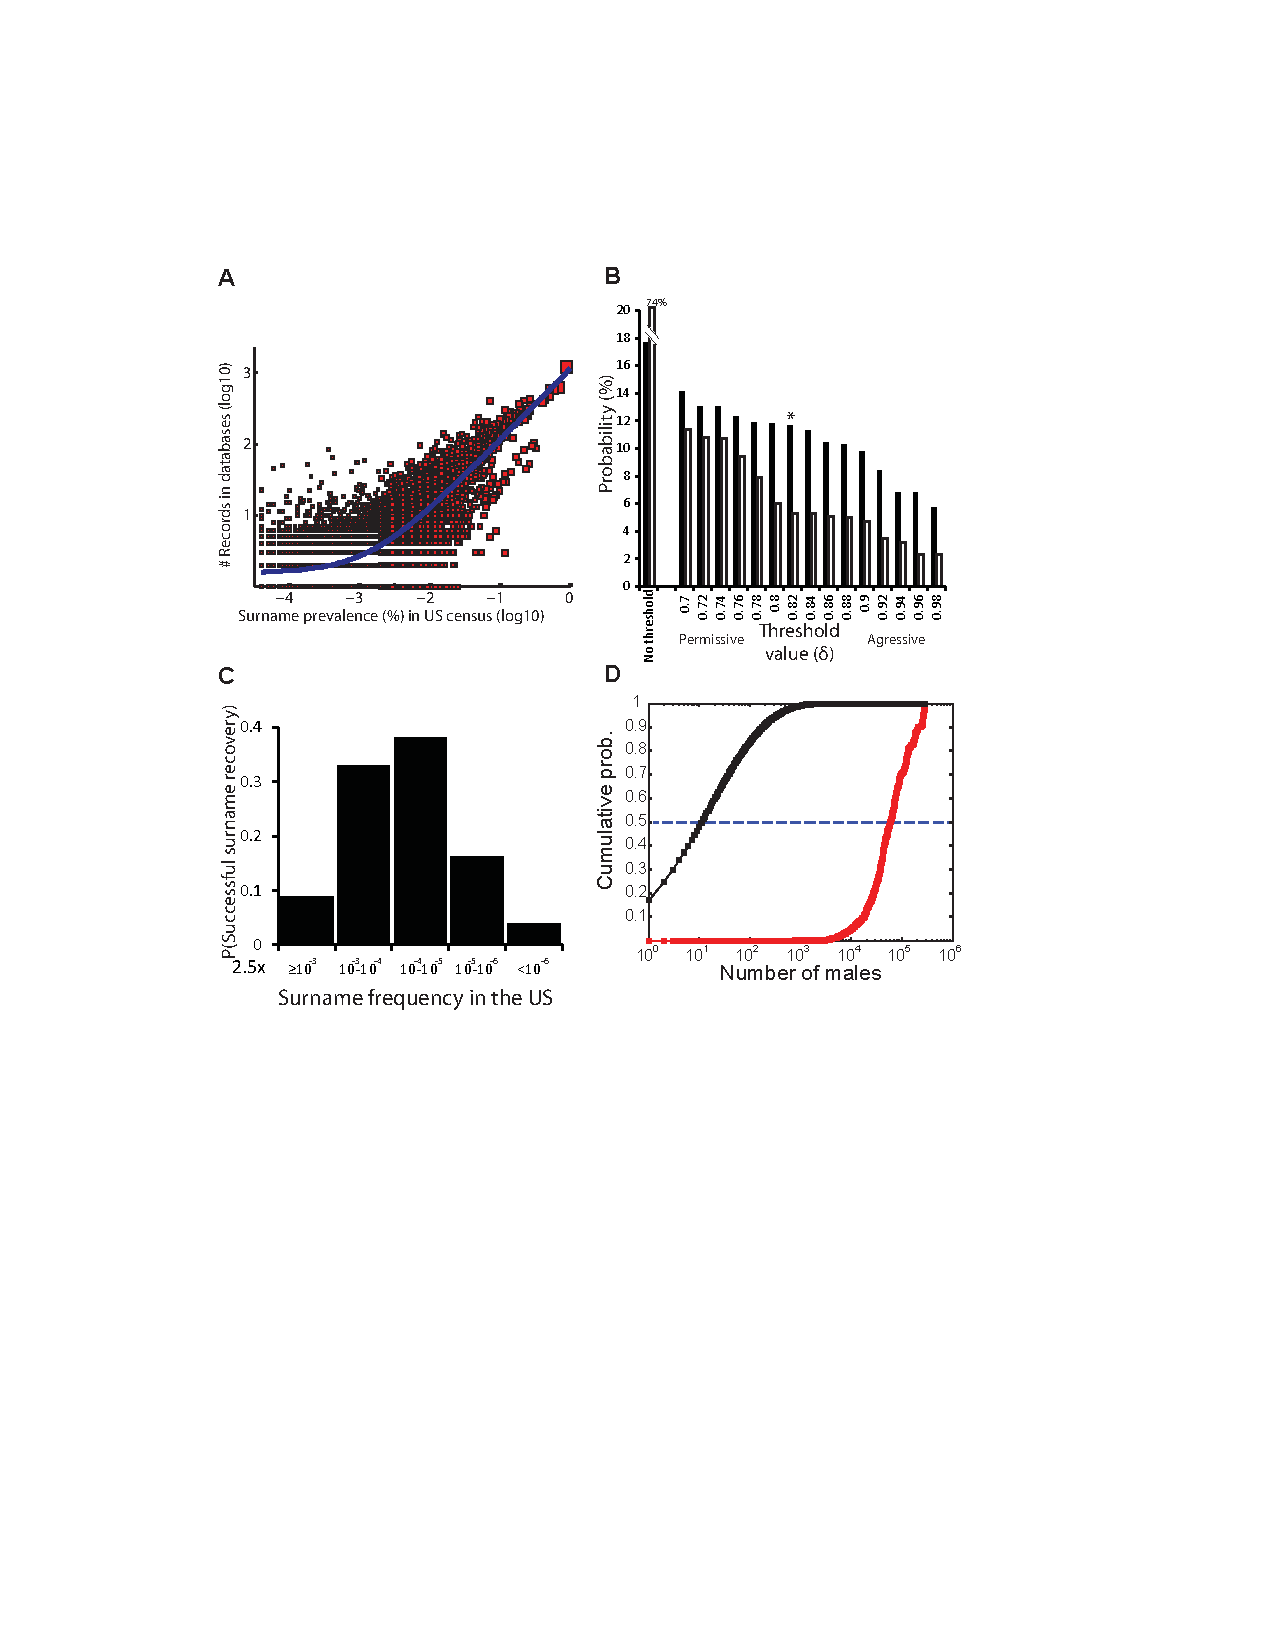
\includegraphics[width=0.5\textwidth]{Figures/App1/Fig1.pdf}
\caption{\textbf{Quantitative assessment of identification via surname inference} \textbf{(A)} The number of Ysearch and SMGF records as a function of surname prevalence in the US population. The best fit line is shown in blue. \textbf{(B)} Expected performance of surname recovery. The probability of successful recovery (closed bars) and wrong recovery (open bars) are shown at different surname confidence thresholds. The star indicates the middle-range performance threshold that was described in the main text. \textbf{(C)} The expected distribution of recovered surnames as a function of their prevalence. Most recovered surnames are expected to have a frequency of 1:4,000 individuals or less. \textbf{(D)} The cumulative distribution function of US males with a profile that matches a specific age, state, and surname combination (black) compared to the distribution when only age and state are known (red). The median is labeled with a dashed line.}
\end{figure}

Next, we established the feasibility of Illumina sequencing to produce accurate Y-STR haplotypes. Using lobSTR, an algorithm for STR profiling from raw sequencing reads \cite{GymrekGolanRossetEtAl2012}, we processed ten high coverage male genomes from the Human Genome Diversity Panel (HGDP). lobSTR produced Y-STR haplotypes with an average length of 53 out of the possible 79 genealogical markers (\textbf{Supplementary Table \ref{fig:sursup5}}). Comparing these results to capillary electrophoresis calls revealed 99\% accuracy. We further found that even at lower sequencing coverage of 10x, informative haplotypes can be obtained by lobSTR (\textbf{Supplementary Figure \ref{fig:sursup4}}). To test the ability to retrieve genetic genealogy records with the Illumina haplotypes, we profiled STRs from the genome of a US Caucasian male from our lab collection that was sequenced with Illumina 100bp reads to a coverage of 13x. In parallel, we submitted this sample to the genealogy service of Sorenson Genomics and created a Ysearch record based on their results. A search with the Illumina haplotype returned his Ysearch entry as a top record (\textbf{Supplementary Figure \ref{fig:sursup5}}).

The NCBI archives host a small number of genomes from identified individuals, providing good test cases for identification via surname inference. We used lobSTR to extract Y-STR haplotypes from the genomes of John West \cite{LeatEhrenreichBenjeddouEtAl2007}, Michael Snyder \cite{LimXueParkinEtAl2007}, and Craig Venter \cite{LevySuttonNgEtAl2007} (\textbf{Supplementary Table \ref{fig:sursup6}}). Searching Ysearch and SMGF with the Y-STR haplotypes of West and Snyder did not return their surnames and resulted in low matches to records with relatively ancient MRCAs 23-28 generations ago (\textbf{Supplementary Material \ref{sec:sursm}}). A search with Craig Venter's haplotype returned a clear match to a ``Venter'' record that was concordant at all 33 comparable markers and with an estimated TMRCA of less than 8 generations (\textbf{Figure \ref{fig:surfig2}}). We further tested whether it would be feasible to trace back Craig Venter by combining his surname with demographic profiling. A query for ``Surname: Venter, Year of Birth: 1946, State: California'' in online public record search engines retrieved two matching records of males, one of whom was Craig Venter himself. 

Surname inference from personal genomes puts the privacy of current de-identified public datasets at risk. We focused on the male genomes in the collection of Utah Residents with Northern and Western European Ancestry (CEU). The informed consent of these individuals did not definitively guarantee their privacy and stated that futuristic techniques might be able to identify them \url{http://hapmap.ncbi.nlm.nih.gov/downloads/elsi/CEPH_Reconsent_Form.pdf}. To test the ability to trace back the identities of these samples from personal genomes, we processed with lobSTR 32 Illumina genomes of CEU male founders that reside in public repositories of the 1000 Genomes Project \cite{AbecasisAltshulerAutonEtAl2010} and the European Nucleotide Archive that were sequenced with read lengths of at least 76bp. Most of these genomes were sequenced to a shallow depth of less than 5x, and produced sparse Y-STR haplotypes. We selected the ten genomes that had the longest Y-STR haplotypes with a range of 34-68 markers to attempt surname recovery. Searching the genetic genealogy databases returned top-matching records with Mormon ancestry in 8 of the 10 individuals for which the top hit had at least 12 comparable markers. Moreover, for four individuals, the top match consisted of multiple records with the same surname, increasing the confidence that the correct surname was retrieved. This potential high surname recovery rate stems from a combination of the deep interest in genetic genealogy among this population and the large family sizes, which exponentially increases the number of targeted individuals for every person that is tested. 

\begin{figure}[h!]
\centering
\label{fig:surfig2}
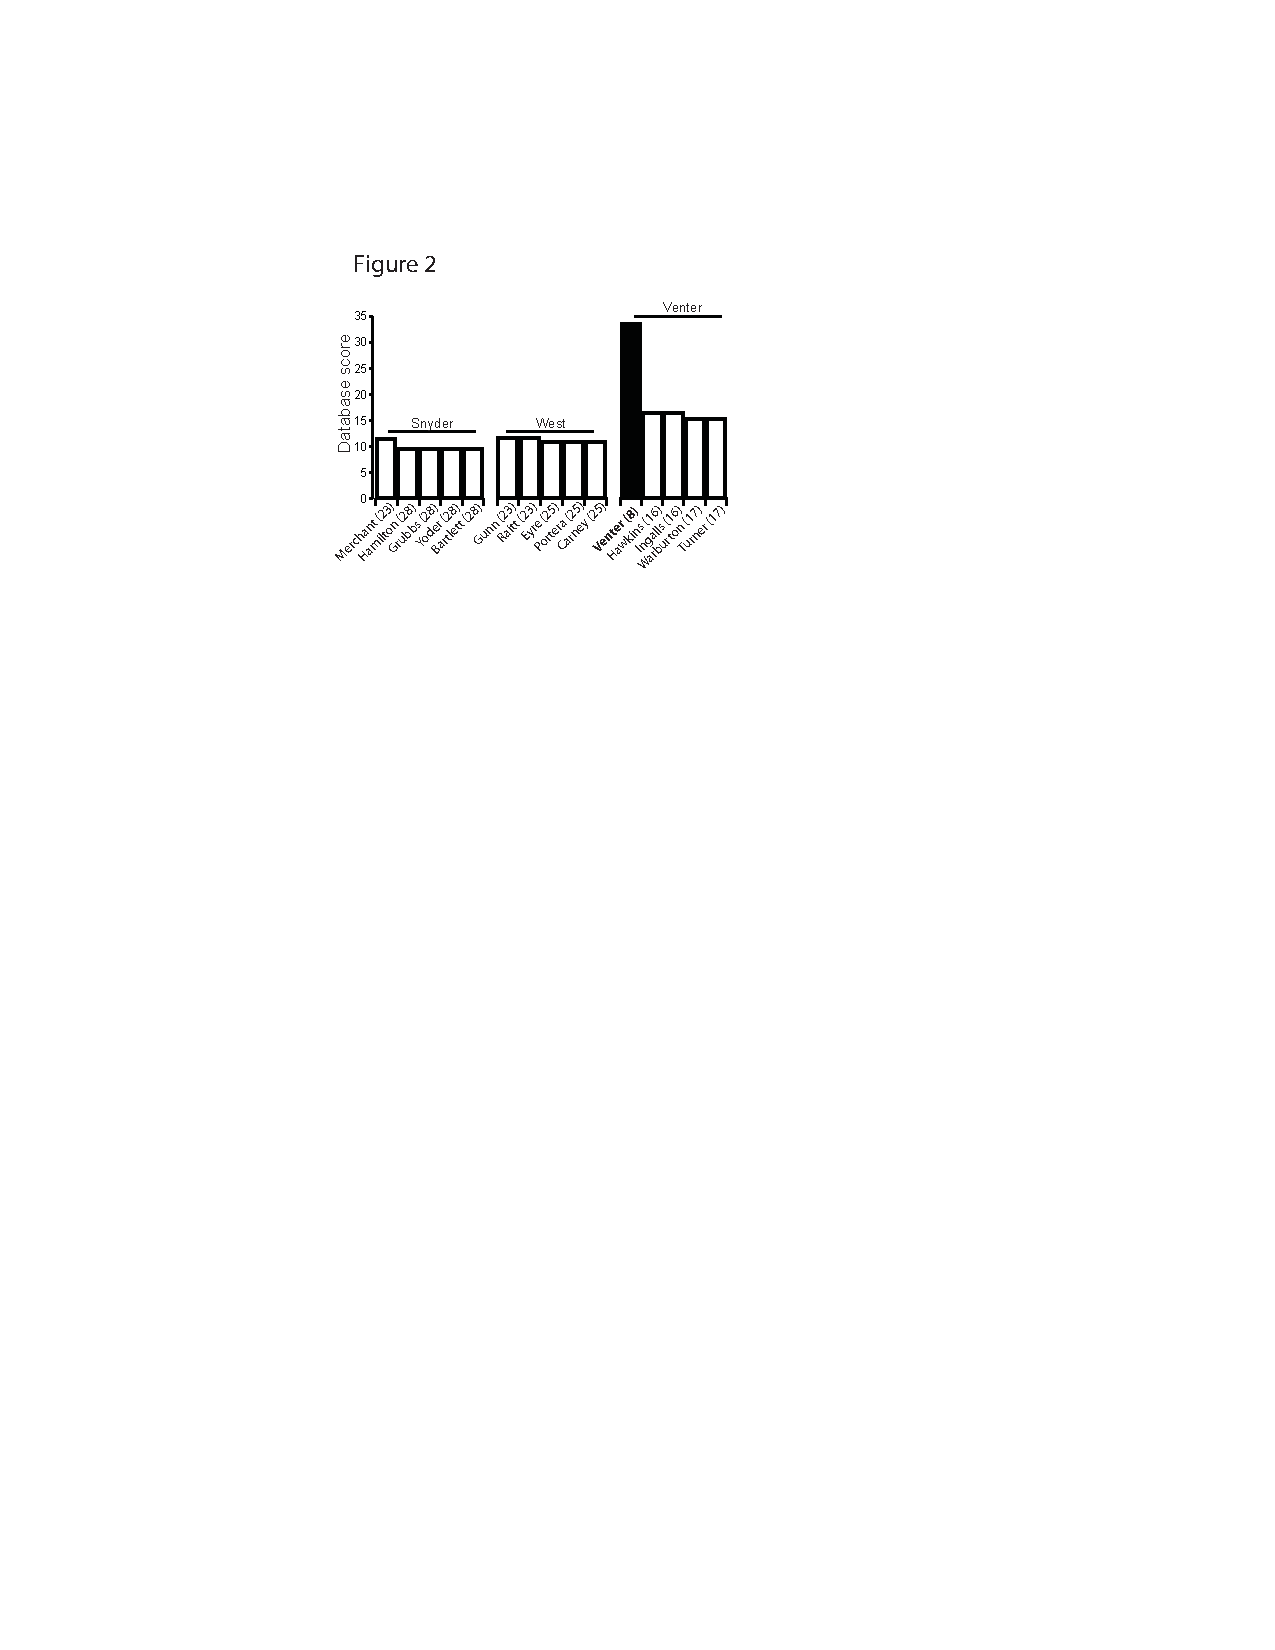
\includegraphics[width=0.5\textwidth]{Figures/App1/Fig2.pdf}
\caption{\textbf{The top five records retrieved after searching Ysearch with the Y-STR haplotypes of Michael Snyder, John West, and Craig Venter.} The expected number of generations to the MRCA is given in parentheses for each record. Searching with Craig Venter returned a ``Venter'' record (closed bar) as the top match.}
\end{figure}

In five surname recovery cases, we fully identified the CEU individuals and their entire families with very high probabilities (\textbf{Table \ref{tab:surtab1}}). These five cases belonged to three pedigrees, where in two of these pedigrees the surnames of both the paternal and maternal grandfathers were recovered. Our strategy for tracing back individuals relied on the recovered surnames as well as publicly available Internet resources such as record search engines, obituaries, and genealogical websites, and demographic metadata available in the Coriell Cell Repository website. The year of birth was inferred by subtracting the ages in Coriell from the year of collecting samples. Each search took 3 to 7 hours by a single person. The identified families matched exactly to the corresponding pedigree descriptions in the Coriell database: the number of children, the birth order of daughters and sons, and the state of residence were identical. All grandparents were alive in 1984, the year that the CEU cell line collection was established \cite{PrescottLalouelLeppert2008}. In the two cases of a dual surname recovery from both grandfathers, the surname of the father and the maiden name of the mother matched exactly to the grandfathers' surnames, substantially increasing the confidence of the recovery. Coriell also lists the ages during sample collection for these two pedigrees, which agreed with the age differences of the identified family members. Using genealogical websites, we traced the patrilineal lineage that connects each identified genome through the MRCA to the record originator in the genetic genealogy database (\textbf{Fig. \ref{fig:surfig3}}). This analysis revealed that two to seven meiosis events link the CEU genome to the record source. Finally, we calculated that the probability of finding random families in the Utah population with these exact demographic characteristics is less than 1 in 105-109 (\textbf{Supplementary Material \ref{sec:sursm}}). In total, surname inference breached the privacy of nearly 50 individuals from these three pedigrees.

This study shows that data release, even of a few markers, by one person can spread through deep genealogical ties and lead to the identification of another person who might have no acquaintance with the person who released his genetic data. The propagation of information through shared male lines amplifies the range of identification, allowing $\sim$135,000 records to potentially target several millions of US males. Another feature of this identification technique is that it entirely relies on free, publicly-available resources. It can be completed end-to-end with only computational tools and an Internet connection. The compatibility of our technique with public record search engines makes it much easier to continue identifying other datasets in the same pedigree, including female genomes, once one male target is identified.  We envision that the risk of surname inference will grow in the future. Genetic genealogy enthusiasts add thousands of records to these databases every month. In addition, the advent of third-generation sequencing platforms with longer reads will enable even higher coverage of Y-STR markers, further strengthening the ability to link haplotypes and surnames.

\begin{figure}[h!]
\centering
\label{fig:surfig3}
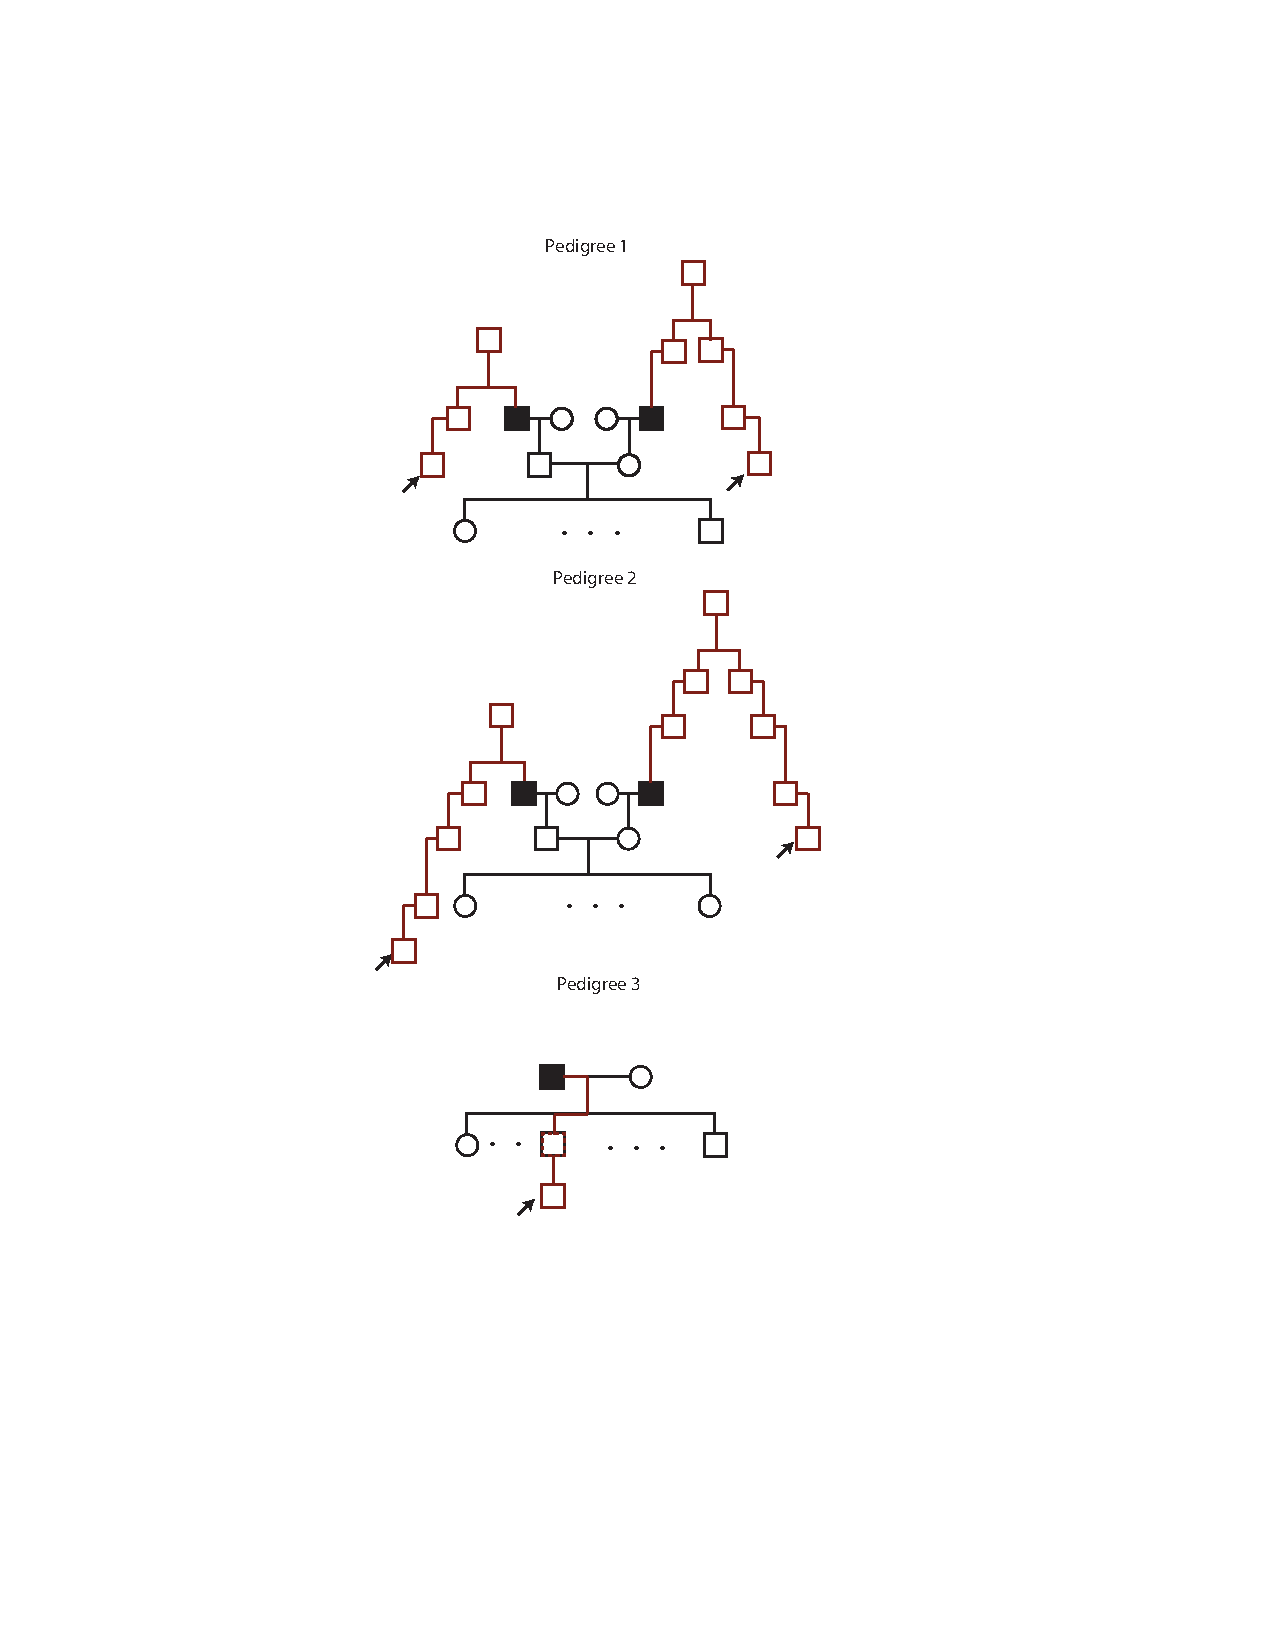
\includegraphics[width=0.5\textwidth]{Figures/App1/Fig3.pdf}
\caption{\textbf{Illustrations of the three CEU pedigrees (black) showing how genetic information from distant patrilineal relatives (arrow; red - patrilineal lines) can identify individuals.} Filled rectangles represent sequenced individuals. To respect the privacy of these families, only abbreviated versions are presented. The sex of the CEU grandchildren was randomized.  The numbers of grandchildren are not given.}
\end{figure}

Similar to other genetic privacy issues \cite{LinOwenAltman2004,BieberBrennerLazer2006,HomerSzelingerRedmanEtAl2008,JacobsYeagerWacholderEtAl2009,ImGamazonNicolaeEtAl2012,CraigGoorWangEtAl2011,SchadtWooHao2012}, preventing surname inference from public whole genome datasets might be quite challenging. Masking Y-STR markers could limit the effectiveness of the method presented in this study, but this approach is not sustainable (\textbf{Supplementary Material \ref{sec:sursm}}). Our analysis suggests that Y-STR haplotypes can be imputed back from SNPs on the Y-chromosome (Y-SNPs) when a large reference set of male genomes will be available (\textbf{Supplementary Figure \ref{fig:sursup6}}). In addition, community efforts, such as the Y Chromosome Genome Comparison, have already started exploring the association between Y-SNPs and surnames (\textbf{Supplementary Table \ref{tab:sursuptab1}}), and might allow bypassing Y-STR masking. We also posit that restricting genetic genealogy information is not practical as some of the data is already scattered in multiple end-user websites and genealogy mailing lists. 

Existing policy tools, such as controlled access databases with data use agreements, may mediate the exposure of genomic information to surname inference. However, in our view, the appropriate response to genetic privacy challenges such as these is not for the public to stop donating samples or for data sharing to stop - which would be devastating reactions that could significantly hamper scientific progress. Rather, we believe that establishing clear policies for data sharing, educating participants about the benefits and risks of genetic studies \cite{McGuireGibbs2006} and the legislation of proper usage of genetic information are pivotal ingredients to support the genomic endeavor.

\begin{figure}[h!]
\centering
\label{tab:surtab1}
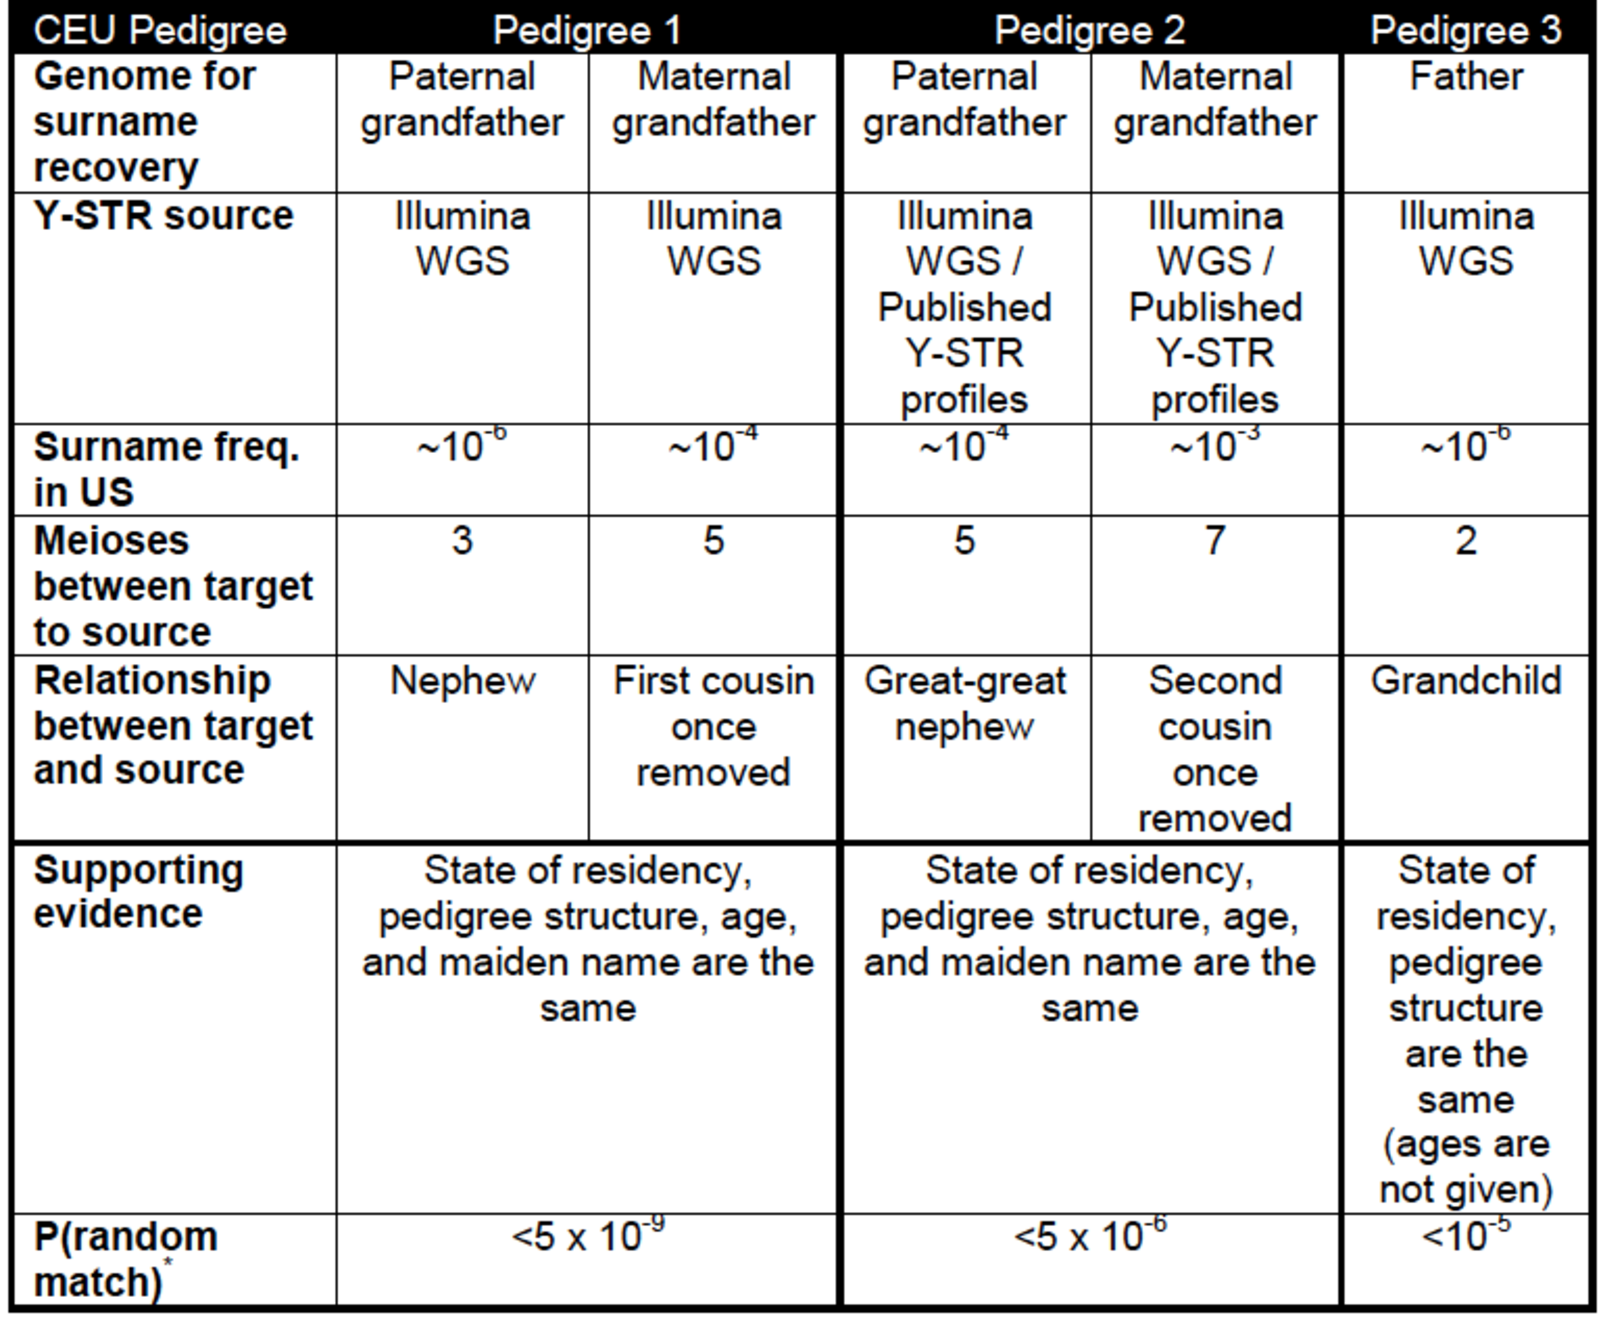
\includegraphics[width=0.9\textwidth]{Figures/App1/Table1.pdf}
\caption{\textbf{Comparison of CEU identification cases.}}
\end{figure}

\section{Acknowledgements}
We thank FamilyTreeDNA and SMGF for technical assistance. The authors would like also to thank Dina Esposito, Alon Goren, Gerry Fink, David Page, Wendy Kramer, and Roy Ronen, for useful discussions. Y.E. is an Andria and Paul Heafy Family Fellow. This publication was supported by the National Defense Science and Engineering Graduate Fellowship (M.G.) and by the Edmond J. Safra Center for Bioinformatics at Tel-Aviv University (D.G. and E.H.). 

\section{Supplementary Material}
\label{sec:sursm}

\subsection{Evaluating the general risk of surname recovery}
\subsubsection{Downloading Ysearch data}
The Ysearch website belongs to FamilyTreeDNA (FTDNA), a Texas-based genetic genealogy company. The website allows users, regardless of their testing service, to voluntarily post their Y-STR genotyping results along with their ancestral information and contact details. Based on the data posted on the website, approximately 85\% of Ysearch's users were tested with FamilyTreeDNA and the other 15\% were tested with other genetic genealogy services. Users from other services are advised to post their results using FamilyTreeDNA nomenclature, and the website offers a conversion table between popular genetic genealogy services and FamilyTreeDNA nomenclature.

With permission from FamilyTreeDNA, we scraped the entire Ysearch database in May 2011. Some areas are protected by reCaptcha and were accessed manually. After parsing and merging the HTML files, we obtained 95,000 surname-haplotype entries, each of which contained: Ysearch userID, surname, ancestral location, and Y-STR results. 

\subsubsection{Access to the SMGF database}
The SMGF website belongs to the Sorenson Molecular Genealogy Foundation, a Utah-based non-profit genetic genealogy organization that was recently acquired by Ancestry.com. The website allows users to query the SMGF database but not to create new records, and all records are from the SMGF program. Unlike the Ysearch database, we could not download the database records to our server. With permission from SMGF, we conducted massive queries of their database using an automatic script. The webpages that contained the top 10 results based on the SMGF matching algorithm were downloaded and parsed to identify the matches. 

\subsubsection{Concordance between genealogical databases and the US population}
The surname distribution in the general US population was estimated using the Census 2000 study that is based on 270 million records (\url{http://www.census.gov/genealogy/www/data/2000surnames/index.html}). The Census study lists 151,671 surnames along with their relative prevalence in the general population and ethnic composition in sorted order. To protect the privacy of the participants and due to sample size limitations, the Census data stops when the cumulative frequency of the surnames reaches 90\%, and does not include surnames that are found in less than 100 individuals each. 

We compared the surname distribution in Ysearch and SMGF to the distribution in the general US population in order to evaluate the completeness of the databases. We defined the census coverage probability, denoted by $c$, as the chance that the surname of an individual drawn at random from the US population has at least a single haplotype record in one of these databases, and found that $c$=68.5\%. The correlation between the US population and the genealogical records was evaluated by a permutation test with 10,000 repetitions. We obtained the following statistics: $E[SSE_{permutations}]=9.01 \times 10^6$, $\sigma(SSE_{permutations})=2437$. The hypothesis $SSE$ was $1.99 \times 10^6$. The p-value was calculated using one-sided Chebyshev bound.

\subsubsection{A mathematical model for surname leakage risk}

\emph{Search method}

Our database search method relied on finding a record that shares the closest Time to Most Recent Common Ancestor (TMRCA) with the queried haplotype. The rationale behind this strategy is that close patrilineal relatives have a higher probability of sharing the same surname. For instance, one can imagine that monozygotic twins have a high probability of sharing the same surname, whereas a pair of Y chromosomes whose MRCA lived before the formation of the surname system would have a low probability of sharing the same surname. 

Walsh \cite{Walsh2001} has proposed several Bayesian models for estimating the distribution of the TMRCA in non-recombining haplotypes. We used his ``infinite alleles model with differential mutation rates''. Consider two Y chromosome haplotypes with $n$ STR loci denoted by $\vec{v}=(v_1,v_2,\hdots,v_n)$ and $\vec{u}=(u_1,u_2,\hdots,u_n)$, with vector elements corresponding to the allele lengths. Let $\vec{x} = (x_1,x_2,\hdots,x_n)$ be a binary vector with $x_i=1$ for a match at the $i$-th locus of $\vec{v}$ and $\vec{u}$, and $x_i=0$ otherwise, and let $\vec{\mu}=(\mu_1,\mu_2,\hdots,\mu_n)$ be a vector whose elements denote the probability of a mutation per meiosis in each marker. According to Walsh's model, the probability distribution function (PDF) of the TMRCA between the two haplotypes is:

\begin{equation}
\label{eq:sureq1}
P(t|\vec{x},\vec{\mu}, N_e) = \frac{e^{-t(\frac{1}{N_e}+2\sum_{i=1}^n\mu_ix_i)}\Pi_{i=1}^n(1-e^{-2t\mu_i})^{(1-x_i)}}{I(\vec{x},\vec{\mu},N_e)}
\end{equation}

where $N_e$ is the effective male population size, and $I$ is a normalization factor to ensure that $\sum_{t=0}^{\infty}P(t|\vec{x},\vec{\mu},N_e)=1$. Following Thomson et al. \cite{ThomsonPritchardShenEtAl2000}, $N_e$ was set to 10,000 males. The mutation rates were obtained from the extensive study of Ballantyne, et al \cite{BallantyneGoedbloedFangEtAl2010}.

The expected TMRCA is denoted by τ and is given by:

\begin{equation}
\tau = \sum_{t=0}^{\infty}t_i P(t_i|\vec{x}, \vec{\mu}, N_e)
\end{equation}

The recovered surname was selected according to the record that has the minimal $\tau$ to the searched haplotype. Due to technical constraints with the web queries to SMGF and in order to reduce the amount of calculations, we did not determine $\tau$ for each of the hundreds of thousands of users in the databases. Instead, we employed the following procedure: (i) Ysearch - identify a set of candidate records that have the maximal number of matching markers to the queried haplotype (ii) SMGF – use the native SMGF search tool to identify the top 10 candidates according to the website's proprietary algorithm (iii) Both – calculate $\tau$ for top candidates in Ysearch and SMGF using Eq. \ref{eq:sureq1}, and select the record with the minimal $\tau$ of the searched haplotype. 

\emph{Retrieval confidence score}

The retrieval confidence score determined the probability that the TMRCA of the retrieved record is indeed shorter than that of (i) a record with a distinct surname that has the second to shortest TMRCA and (ii) a random person from the population. Let $P_1$ and $P_2$ be the TMRCA PDFs of the best record and second best record according to Eq. \ref{eq:sureq1}, and let P3 be the PDF of coalescent in a Fisher-Wright population: $P_3 (t|N_e)=N_e^{-1} e^{-N_e t}$. In addition, let $F_i$ be the cumulative probability distribution function of $P_i$. The retrieval confidence score, $\delta$, is given by:

\begin{equation}
\delta(P_1,P_2,P_e) = \sum_{j_1=1}^TP_1(j_1)
\Bigg(
\sum_{j_2>j_1}^TP_2(j_2)
 \Big(
 \sum_{j_3>j_1}^TP_3(j_3)
 \Big)
\Bigg) = \sum_{j=1}^TP_1(j)(1-F_2(j))(1-F_3(j))
\end{equation}

$T$ is the number of generations that is practical for the patrilineal surname system and was set to 20 generations, corresponding to $\sim$1400 AD. $P_2$ was obtained by scanning records in the list that was generated in step (iii); candidate records with less than 20 markers were excluded as well as records with surnames that matched the top hit.

\emph{Surname inference}

We set a threshold, $\delta_0$, which denotes the minimal accepted quality for valid surname recovery. If the retrieval passed the confidence threshold, the algorithm inferred that the record's surname is the surname of the input haplotype. Otherwise, the algorithm rejected the inference and returned ``Unknown''. 1.8\% of the searches returned records with an empty surname field or with strings that are not found in the surname list of the US census such as ``AshkenaziJewishModal''. The algorithm reported these cases as ``Unknown'' as well. Finally, TMRCA ties between two or more records with distinct surnames were also treated as ``Unknown''. 

A surname inference resulted in one of the following outcomes: success – the recovered surname is concordant with the true surname, wrong – the recovered surname does not match the true surname, unknown – below confidence threshold, non-valid surnames, and ties.  

Following previous record linkage studies \cite{GrannisOverhageMcDonald2004,Winkler1995}, successful recoveries included a small number of cases where the returned surname displayed a minute spelling variant from the true one, such as Abernathy and Abernethy. These cases can still direct the adversary in tracing back the target at the price of searching for a larger number of individuals. We adopted a stringent approach to detect spelling variants that required that the first letter of both surnames be identical and that the Jaro-Winkler string distance \cite{Winkler1995} of the surnames be at least 0.9. This relies on the observation that the suffix of a surname is more prone to mutate than the prefix \cite{Winkler1995}. Two percent of the queries showed spelling variants using this approach and they are summarized in the following table:

\begin{table}[h!]
\begin{tabular}{|l|l|l|}
\hline
True surname & Retrieved surname & Jaro-Winkler distance \\
\hline
ABERNATHY    & ABERNETHY    & 0.977 \\
AYRES        & AYERS        & 0.96  \\
BAIRD        & BEARD        & 0.933 \\
BRALLEY      & BRAWLEY      & 0.947 \\
BRITTON      & BRITTAIN     & 0.944 \\
CHRISTIE     & CHRISTISON   & 0.94  \\
CLARK        & CLARKE       & 0.967 \\
COLLISON     & CULLISON     & 0.964 \\
DENNEY       & DENNY        & 0.967 \\
DUFF         & DUFFEL       & 0.933 \\
FLICKINGER   & FLUCKIGER    & 0.93  \\
MCMURTRY     & MCMURTREY    & 0.984 \\
MILLICAN     & MILLIKEN     & 0.937 \\
PALLETT      & PARLETTE     & 0.919 \\
PARLET       & PARLETTE     & 0.956 \\
SAYRE        & SAYER        & 0.961 \\
SEELYE       & SEELY        & 0.967 \\
WETHERINGTON & WITHERINGTON & 0.961 \\
\hline
\end{tabular}
\end{table}

Manual inspection of the genealogical records showed that in a large number of these cases the users indicated the spelling variant as an alternative ancestral surname.

The general risk of surname leakage from personal genomes is dictated by three factors: the prior distribution of surnames in personal genomes datasets, the distribution of haplotypes within a surname, and the ability to successfully retrieve the surname from the database using the haplotype. For simplicity, we assumed that the distribution of surnames of personal genomes is similar to the distribution of surnames in the population. 

Let $I_x(h,s)$ be an indicator function that returns 1 if querying the database with the combination of haplotype $h$ and surname s returns the outcome $x$, where $x$ is either: ``success'', ``wrong'', or ``unknown''. Let $f_s$ be the frequency of a surname and α(h,s) be the frequency of haplotype $h$ in the surname $s$. Define $\beta_x(s) = \sum_{h \in H(s)} \alpha(h,s)I_x(h,s)$, where $H(s)$ is the set of haplotypes that are associated with the surname $s$. The probability of the surname recovery outcome x for a given population is:

\begin{equation}
\label{eq:sureq3}
P(x) = \frac
{\sum_{s \in S} f_s \beta_x(s)}
{\sum_{s \in S} f_s}
\end{equation}

Where $S$ is the set of all surnames in the population. The probability in Eq. \ref{eq:sureq3} can be assessed by sampling individuals from the population using the following estimator:

\begin{equation}
\label{eq:sureq4}
P(x) = 
\frac{\sum_{s \in S} \hat{f}_s \hat{\beta}_x(s)}
{\sum_{s \in S}\hat{f}_s}c + 
\frac{\sum_{s \in \overline{S}} \hat{f}_s\hat{\beta}_x(s)}
{\sum_{s \in \overline{S}} \hat{f}_s} (1-c)
\end{equation}

where $S$ is the set of surnames in the sample that are known to be present in the tested databases and $\overline{S}$ is the set of surnames in the sample that are known to be absent from the tested databases. $\hat{f}_s$ is the estimated frequency of the surname based on the Census data, $\hat{\beta}_x(s) = \sum_{h \in H(s)} \hat{\alpha}(h,s)I_x(h,s)$ and $\hat{\alpha}(h,s)$  is the frequency of the haplotype-surname combination in the sample, and $c$ is the census coverage probability that was determined above. Eq. \ref{eq:sureq4} models the outcome rates as a weighted sum of sampling individuals from two distinct strata: those whose surname is found in the databases and those who do not. The two weights mitigate potential ascertainment biases in the sample and increase the confidence that the results reflect the target population.

\subsubsection{Estimating the risk of surname leakage by inter-database comparisons}
Our input sample relied on a cohort of individuals from the YBase database. This database was maintained by DNA Heritage and was acquired by FamilyTreeDNA in April 2011. FamilyTreeDNA provided us with surname-haplotype records from the database, without other identifiers that can expose the identity of the database users. The YBase and SMGF entries are completely distinct because the SMGF database lists only SMGF users. We took the following steps to remove potential duplicate records between Ysearch and Ybase: first, we asked FamilyTreeDNA to exclude YBase entries whose email addresses appear in Ysearch as well as entries without email addresses. Second, we removed from the downloaded copy of Ysearch all $\sim$900 users that were tested with DNA Heritage. Third, we excluded any YBase user whose haplotype did not show a combination of markers that are typical to the DNA Heritage test panel. Thus, the input cohort was tested with a different company (DNA Heritage) than the database users. This reduces the chance of ascertainment biases due to oversampling of close relatives of the database participants.

Genetic genealogy databases are subject to nomenclature heterogeneity that can confound the analysis. This is especially problematic for DNA Heritage test panels that were subject to five nomenclature changes between 2003 to 2009 (see: \url{http://web.archive.org/web/20100307032155/http://www.dnaheritage.com/helpfiles/DNA_Heritage_nomenclature_changes.pdf}). For each input haplotype, we inspected the allelic ranges for markers that underwent significant nomenclature changes, such as DYS452, to decipher the nomenclature stratum and to standardize the haplotype according to the NIST recommended nomenclature. In addition, we set a tolerable genotype range for each marker that is equal to the marker mean value in Ysearch$\pm$3std. Entries outside of this range have a high likelihood of nomenclature differences and typos of users. This step filtered approximately 5\% of YBase haplotypes. Finally, we selected only YBase haplotypes that have full genotyping results for a set of 34 STR markers (\textbf{Supplementary Table \ref{tab:sursuptab2}}) and whose surnames are in the US census. At the end of this process, we retained 911 YBase records.

We used a series of Perl scripts to challenge Ysearch and SMGF with the YBase haplotypes and to compare the returned surnames to the true ones. SMGF searches were conducted with the NIST nomenclature and Ysearch searches were conducted with FamilyTreeDNA nomenclature. The standard deviation was calculated by 30 iterations of re-sampling with replacement participants from the input cohort and repeating the analysis process.

The results of the 911 queries exhibited distinct patterns between the TMRCA of records that exactly match the true surname, records with a spelling variant, and records that returned the wrong surnames (\textbf{Supplementary Figure \ref{fig:sursup1}}). The mean TMRCA was 10.3 generations for exact matches, 15.6 generations for a spelling variant, and 24.3 generations for wrong surnames. The TMRCA distribution of exact matches appeared to follow a geometric distribution trend. The TRMCA of records with spelling variants was almost never more recent than 10 generations and was quite different from the distribution of wrong matches. This provides another support for our spelling variations detection algorithm. \textbf{Supplementary Figure \ref{fig:sursup2}} shows the final results after processing the results according to Eq. \ref{eq:sureq4}.

\subsection{From Surnames To Individuals}
\subsubsection{The frequency distribution of leaked surnames}
We determined the frequency distribution of leaked surnames from the YBase simulations using the following equation:

\begin{equation}
\label{eq:sureq5}
P(s \in S_i | x = success, \delta) = \frac
{P(x=success | s \in S_i, \delta)P(s \in S_i)}
{P(x=success | \delta)}
\end{equation}

Where $S_i$ is a subset of surnames whose frequencies fall in the $i$-th bin out of $j$ possible bins. Specifically, we used the following bins:

\begin{table}[h!]
\begin{tabular}{|l|l|l|}
\hline
Bin(i) & Frequency boudnaries & Example of surnames in bin \\
\hline
1& 	$>$1:400 &	Smith, Johnson \\
2	&1:400 – 1:4,000	& Turner, Collins\\
3	& 1:4,000 – 1:40,000 & 	Gates, Sloan\\
4	& 1:40,000 – 1:400,000 &	Bjork, Reach \\
5	& $<$1:400,000 &	Kellog, Venter \\
\hline
\end{tabular}
\end{table}

The term $P(s \in S_i)$ in Eq. \ref{eq:sureq5} is given by the census data. The other numerator term can be approximated using a slight modification to Eq. \ref{eq:sureq4}:

\begin{equation}
\label{eq:sureq6}
P(x = success | s \in S_i, \delta) = 
\frac{\sum_{s \in S} \hat{f}_s \hat{\beta}_x(s)}
{\sum_{s \in S}\hat{f}_s}c_i + 
\frac{\sum_{s \in \overline{S}} \hat{f}_s\hat{\beta}_x(s)}
{\sum_{s \in \overline{S}} \hat{f}_s} (1-c_i)
\end{equation}

Where $c_i$ is a normalization factor that denotes the probability that a random person from the US population whose surname is in the $i$-th bin has at least a single entry in Ysearch and SMGF.  $c_i$ was determined by intersecting the census data with the list of Ysearch and SMGF. We used $\delta$=0.82.

The leaked surnames are mostly found in the intermediate bin with a frequency of 1:4,000-1:40,000. Extremely rare surnames have the lowest relative risk for leakage due to the absence of records in Ysearch and SMGF. However, if these databases have even a single record for an extremely rare surname, then there is a 43\% chance that the surname will be exposed (\textbf{Supplementary Figure \ref{fig:sursup3}}). This phenomenon is potentially due to the small number of male lineages in extremely rare surnames.	

\subsubsection{Combining surnames with demographic identifiers}
The joint probabilities of sex, age, and state were obtained from the US Census Population Estimates Program (\url{www.census.gov/popest/states/asrh/files/SC-EST2009-AGESEX-RES.csv}). The data is based on Census 2000 and contains a projection of residents to 2009, which was used in the simulation. Similar to the HIPAA law, ages that are over 85 were grouped in a single category. 

The simulation ran 100,000 times. In each round, a combination of state and age was selected according to their probability in the joint distribution. For instance, there are 287,000 males in California who are 25 years old and 3,500 males in Idaho who are 75 years old. Accordingly, the probability of selecting ``California, 25'' was 82 times higher than selecting ``Idaho, 75''. Next, a bin of a leaked surname was selected according to its probability in Eq. \ref{eq:sureq6} and a surname was selected according to its frequency in the bin. For instance, in the case of selecting the 1st bin ($\geq$1:400), Smith had 1.28 higher probability of being sampled than Johnson. Finally, the simulation randomly selected between the return of a spelling variant or exact match, where the former had a probability 11.11\%, based on our empirical findings in the Ybase simulations. In case of no spelling variant, the surname frequency was set to the census frequency; otherwise, the surname frequency was selected to be the sum of frequencies of all surnames that can be spelling variants of the original surname according to our spelling variant definition above. The last step portrays a scenario in which the adversary first looks for the target with the returned surname and if he cannot trace the target back, he tries all spelling variants. The number of expected individuals was found by multiplying the surname frequency by the number of males with the selected age and geographical location.

We validated the results of the simulation by comparing them to real datasets of US residents from PeopleFinders (\url{www.peoplefinders.com}). These datasets are based on extensive mining of public records, such as voter and drivers license registries, and can be searched by a combination of surname, age, and state. We selected 30 random simulation rounds that passed two criteria: (a) the ages were restricted to 25-35 years to avoid potential confounding due to underrepresentation of minors in public records and conflicting records from deceased individuals (b) the expected number of individuals should be 10-100 to avoid overloading the website. In most cases the lists in PeopleFinders were smaller than expected from simulations. Although we cannot rule out incompleteness of the website, the results also suggest that any underestimation of the list size - if it exists at all - is not significant.

\subsection{Profiling Y-STRs from sequencing data}
\subsubsection{lobSTR usage}
Unless otherwise specified, lobSTR v2.0.0 was used to profile Y-STRs from raw whole-genome sequencing data \cite{GymrekGolanRossetEtAl2012}. In brief, lobSTR acts in three steps: detecting reads with repetitive elements that are flanked with non-repetitive regions, aligning the flanking regions to a reference, and measuring the repeat length for each STR. 

\emph{Improved Y-STR reference}

We modified lobSTR's standard STR reference to include the genomic locations and nomenclatures of genealogical Y-STRs. These locations were found by conducting in silico PCR on the UCSC genome browser using published Y-STR primers \cite{KayserKittlerErlerEtAl2004,BoschLeeCalafellEtAl2002,ButlerDeckerValloneEtAl2006,HansonBerdosBallantyne2006,LimXueParkinEtAl2007,LeatEhrenreichBenjeddouEtAl2007,MalaspinaCiminelliViggianoEtAl1997,SchoskeValloneKlineEtAl2004,JoblingSamaraPandyaEtAl1996} and by searching the FamilyTreeDNA Y chromosome browser (\url{ymap.ftdna.com}). Several STR markers reside in duplicated regions of the Y chromosome. For instance, DYS385 has two distinct alleles in a single individual. Since lobSTR filters multi-mappers, we kept only one entry of these markers in the modified reference. Markers DYS448 and DYS449 consist of two STR regions separated by a non-repetitive region. For these, a separate reference entry was created for each region and the final genotype was determined by adding the alleles profiled at each of the two STR regions. 

We did not include eight genealogical markers in the reference due to various technical reasons: markers GAAT1B07 and DYS724a/b (also known as CDYa/b) were excluded because their corresponding genomic coordinates could not be determined despite extensive literature searches.  DYS726 was excluded because the genetic genealogy nomenclature could not be determined. DYS425 is one of the four repetitive loci of DYF371 \cite{JoblingSamaraPandyaEtAl1996}, and using short reads we could not uniquely determine which locus a read originated from. DXYS156-Y was excluded because it is not specific to the Y-chromosome. Marker DYS19b was not included in because it is present in 0.2\% of the population. Marker DYS640 was incorrectly annotated in our original reference and discarded from further analysis. Marker DYS464a-d was excluded because in most cases we typed fewer than four alleles and could not accurately assign typed alleles to forms a-d.  In summary, our reference included 34 out of the 36 markers used by the SMGF panel and 79 out of the 87 markers in the most comprehensive test panel of FamilyTreeDNA. The genomic coordinates and conventions used for each Y-STR are given in \textbf{Supplementary Table \ref{tab:sursuptab3}}). All coordinates reported in this study follow the hg19 human reference build.

\emph{Processing lobSTR calls}

lobSTR returns base pair length differences from the UCSC genome reference. Genetic genealogy services use an STR nomenclature that follows the PCR product sizes according to arbitrary primers \cite{GusmaoButlerCarracedoEtAl2006}. Whenever available we used the NIST nomenclature to translate lobSTR results (\url{http://www.cstl.nist.gov/strbase/ystr_fact.htm}). For searches in the Ysearch database results were converted to FamilyTreeDNA nomenclature using a conversion table available from SMGF (\url{http://www.smgf.org/ychromosome/marker_standards.jspx}). 

For Y-STRs with a single genomic location, the allele with the modal number of supporting reads was used. Y-STR alleles that showed a non-integer number of repeat copies were discarded. We manually inspected a small number of calls where the modal allele was supported by less than 60\% of reads aligned to the locus and enhanced the call by removing reads likely to be erroneous, such as reads that contain a high number of sequence mismatches, reads in which the STR resides towards the end of the read, or reads supporting alleles outside the normal range. Importantly, this procedure was executed completely blind to the true allele if it was known. For bi-mapper markers, such as DYS413a/b, the shortest repeat length was assigned to allele ``a'' and the next to allele ``b''. 

\subsubsection{Comparing lobSTR to the CEPH Y-STR panel}

\emph{General approach}

Sequence data for the CEPH panel were downloaded from the NCBI Short Read Archive from experiment SRP009145, sample SRS269343, runs SRX103805-130812. The sample included 10 HGDP individuals: HGDP00456 (Mbuti Pygmy), HGDP00665 (Sardinian), HGDP01284 (Mandenka), HGDP00542 (Papuan), HGDP00521 (French), HGDP00778 (Han Chinese), HGDP01307 (Dai), HGDP00927 (Yoruba), HGDP01029 (San), HGDP00998 (Karitiana). Autosomal coverage was calculated using the samtools \cite{LiHandsakerWysokerEtAl2009} depth tool and gives the average depth of covered bases based on alignments using BWA \cite{LiDurbin2009a}. lobSTR 2.0.0 with the improved Y-STR panel was used for the analysis.

Genotypes for 76 Y-STRs typed by capillary electrophoresis for the 10 HGDP samples were obtained from the CEPH website (\url{ftp://ftp.cephb.fr/hgdp_supp9/}). Forty-seven of these markers overlapped with the lobSTR reference and were used to evaluate lobSTR's ability to type Y-STRs.

lobSTR reports alleles as the length difference from the UCSC, whereas the CEPH genotypes are reported as the number of repeat copies at each locus. To convert lobSTR output to the same format, we used for following equation: $r+l/p$, where $r$ is the number of base pairs of the STR of the lobSTR reference, $l$ is the reported lobSTR allele in base-pairs, and $p$ is the period of the Y-STR. For all individuals in which lobSTR recovered a genotype for DYS385a/b, only a single allele was returned. If the returned allele matched either the ``a'' or ``b'' form reported by CEPH, it was considered as correct. This follows our search strategy with the personal genomes, where these partial calls of multi-allelic markers were used to exclude matches not containing the lobSTR call for either allele. 

We noticed that the lobSTR calls for all six individuals typed for DYS481 and all three individuals typed for DYS594 are exactly one repeat away from the results in the CEPH study. There is known nomenclature heterogeneity for these markers and some test kits report them with one shorter repeat than as reported by the NIST standard . Concordantly, we converted lobSTR calls to the shorter allele nomenclature to match that reported by CEPH.

\emph{Number of markers profiled at different sequencing coverage levels}

Based on our previous experience with lobSTR, we assumed that STR coverage is linearly related to autosomal coverage. For each genome, we used the Picard (\url{http://picard.sourceforge.net}) DownsampleSam tool to randomly down-sample reads from the lobSTR alignment file to simulate coverage levels corresponding to autosomal coverage ranging from 1x to 25x. For each coverage level, we repeated the lobSTR allelotyping step to call the Y-STRs. The best-fit saturation curve was found using nonlinear least squares to fit a hyperbolic curve and was extended to predict haplotype lengths for up to 50x coverage.

\emph{Further investigation of wrong Y-STR calls}

In our previous studies, we found that PCR stutter noise is a major source of error in calling STR alleles. This type of noise usually adds or subtracts a single repeat unit from the true allele. We noticed that the erroneous calls in DYS490 and DYS572 are several repeats away from the true allele, reducing the probability that these errors stem from stutter noise. Further analysis found that these two markers have X chromosome homologs, and that the calling errors can be attributed to misalignment of the X chromosome STRs. We also noticed that these markers were occasionally detected in the female genomes of the CEU panel, which provides further support for this hypothesis. Future algorithm improvements can use the homolog calls from the X chromosome to detect these errors.

\subsection{Cases of Surname Leakage from Personal Genomes}
\subsubsection{Querying genealogical databases}
In all surname recovery experiments from personal genomes, database queries utilized the native search interfaces of the websites. 

Ysearch was queried using the haplotype matching tool available at \url{http://www.ysearch.org/search_search.asp?uid=&freeentry=true}. Online searches were conducted with the default parameters and using the FamilyTreeDNA nomenclature. SMGF was queried using the tool at \url{http://www.smgf.org/ychromosome/search.jspx} with the options ``Search by Match\%) = 85\%'' using the NIST nomenclature.

\subsubsection{Feasibility of record retrievals with Illumina}
\emph{The US male sample from our lab collection}

The sequencing experiment was approved by the MIT Committee on the Use of Humans as Experimental Subjects (COUHES).  To comply with the COUHES approval, we cannot share the specific Y-STR results, since this could lead to identification of the individual. As an alternative, we provide summary statistics of the length distribution of the detected Y-STR makers. 

Four Catch-All buccal swabs (Epicentre, QEC89100) were used to collect the sample according to the manufacturer's protocol. Genomic DNA was obtained by QuickExtract (Epicentre), followed by phenol-chloroform purification and ethanol precipitation. Library preparation was performed according to the standard Illumina protocol. Three runs of 101bp paired-end reads were generated with a GAIIx platform, generating 740 million reads. Autosomal coverage of 13x (after removing PCR duplicates) was measured using a conventional alignment pipeline as previously described \cite{ErlichEdvardsonHodgesEtAl2011}.  \textbf{Supplementary Figure \ref{fig:sursup4}A} shows the overlap between the markers that were detected by Illumina versus the genealogical profile from Sorenson Genomics. textbf{Supplementary Figure \ref{fig:sursup4}B} shows the number of STRs that were detected using Illumina and Sorenson as a function of their lengths. 

\emph{Database retrieval}

For the 10 HGDP samples and the US male sample, we supplemented our downloaded copy of the Ysearch database with capillary electrophoresis results. Retrieval of records was conducted with the same scripts used for the Y-STR simulations described above. As an additional validation for our results, we created a Ysearch record for the US male using the Ysearch.org website that does not disclose the true surname of the sample and consists of the Y-STR makers that are shared between Sorenson Genomics and Ysearch. Again, a search with the default website interface returned our sample as the top match.

\subsubsection{Analyzing Michael Snyder's genome}
Raw reads for the blood-derived and saliva-derived DNA of Michael Snyder's genome were downloaded from the NCBI Sequence Read Archive with accessions SRX097307 and SRX097312, respectively. lobSTR 1.0.6 with the native lobSTR reference was used to process both datasets using 20 processors on a server with four 12-core AMD Opteron 6100 Series. Forty-eight Y-STR calls were generated. All Y-STR calls were concordant between the blood-derived and the saliva-derived samples. 

Ysearch link to search this haplotype:

\url{http://www.ysearch.org/search_results.asp?uid=&freeentry=true&L1=14&L2=0&L3=16&L4=0&L5=10&L6=0&L7=0&L8=11&L9=13&L10=0&L11=0&L12=12&L13=0&L14=15&L15=0&L16=0&L17=11&L18=11&L19=0&L20=0&L21=0&L22=0&L23=0&L24=0&L25=0&L26=0&L27=0&L28=0&L29=0&L30=0&L31=0&L32=0&L33=0&L34=14&L35=18&L36=16&L37=19&L38=0&L39=0&L40=12&L41=10&L54=11&L55=8&L56=0&L57=0&L58=8&L59=11&L60=10&L61=8&L62=10&L63=0&L42=0&L64=22&L65=0&L66=0&L67=11&L68=12&L69=12&L70=0&L71=0&L49=13&L72=26&L73=0&L51=0&L74=13&L75=11&L76=12&L77=0&L78=9&L79=12&L80=11&L43=0&L44=12&L45=12&L46=0&L47=0&L48=13&L50=10&L52=0&L53=0&L81=9&L82=11&L83=14&L84=9&L85=15&L86=12&L87=0&L88=0&L89=0&L90=11&L91=10&L92=11&L93=0&L94=10&L95=11&L96=0&L97=0&L98=0&L99=0&L100=0&min_markers=8&mismatch_type=absolute&mismatches_max=0&mismatches_sliding_starting_marker=8&recaptcha_challenge_field=03AHJ_VutYkPmq2enCrhZuu94gU9-tcPRX33GpxRzVYZGBmnUWrEecYh8jggsJ0SU37BuJhpK_nMfhB0r8QTNBIe-_lpzJtyC3IRZ6SXlIn1Tnwb9vfGNo5ZojEQ8_8OlQgtCuVj5rTLfLLEXi4vr0-uFyo7upKwcsOFnxGg9SkL81vHEnACEx9H8&recaptcha_response_field=Weighthe+resume&haplo=&region=}

SMGF link to search this haplotype:

\url{http://www.smgf.org/ychromosome/search_results.jspx?labStandard=NIST&searchType=genetic&matchPercent=match_85&showCountries=on&showMissingData=on&showAllSurnames=on&DYS385_a=None&DYS385_b=None&DYS426=11&DYS447=None&DYS461=None&DYS388=13&DYS437=None&DYS448=None&DYS462=12&DYS389I=None&DYS438=10&DYS449=None&DYS463=None&DYS389B=None&DYS439=None&DYS452=None&DYS464_a=None&DYS464_b=None&DYS390=None&DYS441=14&DYS454=11&DYS464_c=None&DYS464_d=None&DYS391=10&DYS442=17&DYS455=11&GGAAT1B07=None&DYS392=12&DYS444=13&DYS456=14&YCAII_a=None&YCAII_b=None&DYS393=14&DYS445=10&DYS458=15&YGATAA10=14&DYS394=16&DYS446=None&DYS459_a=None&DYS459_b=None&YGATAC4=None&DYS460=None&YGATAH4=None}

\subsubsection{Analyzing John West's genome}

Raw reads for John West's genome were downloaded from NCBI Sequence Read Archive with accession SRA018104. lobSTR 1.0.6 with the improved Y-STR index using the same hardware settings for Michael Snyder genome. 

Ysearch link to search this haplotype:

\url{http://www.ysearch.org/search_results.asp?uid=&freeentry=true&L1=13&L2=0&L3=14&L4=0&L5=11&L6=11&L7=14&L8=12&L9=12&L10=13&L11=0&L12=13&L13=0&L14=17&L15=0&L16=0&L17=11&L18=10&L19=0&L20=15&L21=0&L22=0&L23=0&L24=0&L25=0&L26=0&L27=0&L28=0&L29=0&L30=11&L31=10&L32=19&L33=23&L34=15&L35=19&L36=17&L37=17&L38=0&L39=0&L40=12&L41=12&L54=11&L55=9&L56=0&L57=0&L58=8&L59=10&L60=10&L61=8&L62=9&L63=10&L42=0&L64=0&L65=0&L66=16&L67=10&L68=12&L69=12&L70=15&L71=0&L49=12&L72=22&L73=0&L51=13&L74=0&L75=11&L76=14&L77=0&L78=0&L79=0&L80=0&L43=12&L44=11&L45=14&L46=0&L47=0&L48=13&L50=13&L52=0&L53=19&L81=9&L82=0&L83=16&L84=9&L85=16&L86=12&L87=11&L88=13&L89=13&L90=11&L91=10&L92=12&L93=0&L94=11&L95=10&L96=0&L97=0&L98=0&L99=0&L100=0&min_markers=8&mismatch_type=absolute&mismatches_max=0&mismatches_sliding_starting_marker=8&recaptcha_challenge_field=03AHJ_VusNldFpOWxRw2dib-HZoXRWEvEIRysd8fba2-AEWcvfROt3W2n0f6ARIuHaqcRgZ1JE92e0aXBEDDpPLRfhPpAYpKvyARJb0FqPs1fP_HPkMw8AiwilCMic_tD_ntx119pL-fmM96E18ekPuaxXIu-0Dw0hIg&recaptcha_response_field=Hcacco+and&haplo=&region=}

SMGF link to search this haplotype:

\url{http://www.smgf.org/ychromosome/search_results.jspx?labStandard=NIST&searchType=genetic&matchPercent=match_85&showCountries=on&showMissingData=on&showAllSurnames=on&DYS385_a=11&DYS385_b=14&DYS426=12&DYS447=None&DYS461=12&DYS388=12&DYS437=15&DYS448=None&DYS462=11&DYS389I=None&DYS438=12&DYS449=None&DYS463=19&DYS389B=None&DYS439=13&DYS452=None&DYS464_a=None&DYS464_b=None&DYS390=None&DYS441=14&DYS454=11&DYS464_c=None&DYS464_d=None&DYS391=11&DYS442=17&DYS455=11&GGAAT1B07=None&DYS392=13&DYS444=12&DYS456=15&YCAII_a=19&YCAII_b=23&DYS393=13&DYS445=13&DYS458=17&YGATAA10=16&DYS394=14&DYS446=13&DYS459_a=None&DYS459_b=None&YGATAC4=None&DYS460=11&YGATAH4=11} 

\subsubsection{Surname recovery using the Craig Venter dataset}
Sequence reads for the Venter genome were downloaded from TraceDB (Genbank accession ABBA00000000). We trimmed the first 50bp of every read due to the high error rate at the beginning of Sanger sequence reads and discarded reads whose length after trimming was less than 100bp. 

At the default settings, lobSTR 2.0.0 with the improved Y-STR index returned 40 Y-STRs after 40 minutes of runtime using the same hardware settings as described above. Markers returning a non-integer number of repeat copies were discarded. 
Ysearch link to search this haplotype:

\url{http://www.ysearch.org/search_search.asp?fail=1&uid=&freeentry=true&L1=0&L2=0&L3=0&L4=0&L5=10&L6=0&L7=0&L8=12&L9=12&L10=12&L11=0&L12=13&L13=0&L14=17&L15=9&L16=0&L17=11&L18=11&L19=0&L20=0&L21=0&L22=0&L23=0&L24=0&L25=0&L26=0&L27=0&L28=0&L29=0&L30=0&L31=0&L32=19&L33=23&L34=0&L35=0&L36=0&L37=17&L38=0&L39=0&L40=12&L41=12&L54=12&L55=9&L56=15&L57=16&L58=9&L59=10&L60=10&L61=8&L62=0&L63=0&L42=0&L64=23&L65=0&L66=16&L67=10&L68=12&L69=0&L70=16&L71=8&L49=0&L72=22&L73=0&L51=0&L74=12&L75=11&L76=0&L77=0&L78=0&L79=13&L80=12&L43=12&L44=11&L45=0&L46=0&L47=0&L48=0&L50=0&L52=0&L53=0&L81=0&L82=0&L83=16&L84=9&L85=0&L86=0&L87=0&L88=0&L89=12&L90=11&L91=0&L92=0&L93=12&L94=11&L95=0&L96=25&L97=0&L98=0&L99=0&L100=0&min_markers=8&mismatch_type=absolute&mismatches_max=0&mismatches_sliding_starting_marker=8&recaptcha_challenge_field=03AHJ_VusyS2psJJIgHViP9Prgl35afzMpQdoc1uJYw3a1I3Lob-ycMFtplYmSlwFUE-GDzsh-4mdVv9uutxFV7-2qugmcKl8jVTG3EnVPwKXNihNKdv-TfVxulspdX1RO-5XhOBVpnPWoZhnxE5OVRCTnXF7fVgXO7TAa-0c-ycvvN9Zp-JDq_Io&recaptcha_response_field=tsshora+infinite&haplo=&region=}

SMGF link to search this haplotype:

\url{http://www.smgf.org/ychromosome/search_results.jspx?labStandard=NIST&searchType=genetic&matchPercent=match_85&showCountries=on&showMissingData=on&showAllSurnames=on&DYS385_a=None&DYS385_b=None&DYS426=12&DYS447=None&DYS461=12&DYS388=12&DYS437=None&DYS448=None&DYS462=11&DYS389I=None&DYS438=12&DYS449=None&DYS463=None&DYS389B=None&DYS439=12&DYS452=None&DYS464_a=None&DYS464_b=None&DYS390=None&DYS441=None&DYS454=11&DYS464_c=None&DYS464_d=None&DYS391=10&DYS442=17&DYS455=11&GGAAT1B07=None&DYS392=13&DYS444=None&DYS456=None&YCAII_a=19&YCAII_b=23&DYS393=None&DYS445=None&DYS458=17&YGATAA10=None&DYS394=None&DYS446=None&DYS459_a=9&DYS459_b=None&YGATAC4=None&DYS460=None&YGATAH4=None}

Querying Ysearch as described above returned the entry VPBT4 with surname ``Venter'' as the top hit. The results, including the trace numbers of supporting reads, are summarized in \textbf{Supplementary Table \ref{tab:sursuptab4}} . Concordant with Craig Venter's paternal roots, the top match was the only Venter record in Ysearch with a UK ancestor. The algorithm did not return any of the other dozen Venter entries with ancestors mostly from Germany and South Africa (\textbf{Supplementary Figure \ref{fig:sursup5}} and \textbf{Supplementary Table \ref{tab:sursuptab5}}), emphasizing the specificity of the recovery.

Demographic profiling was conducted using PeopleFinders and USSearch (\url{www.ussearch.com}). Female names and users that did not exactly match year of birth=1946 were discarded. 

\subsubsection{CEU genomes}
The CEU male datasets were accessed through the 1000Genomes publicly available Amazon S3 bucket and the European Nucleotide Archive. In cases of father-son pairs, we selected the father for further analysis. All datasets were first processed with lobSTR 2.0.0 with the native STR reference. We reran the 18 CEU genomes that returned the largest number of markers with the improved Y-STR panel. Overall, these genomes had longer read lengths of 76-100bp compared to 36-51bp and were therefore more amenable to STR calling. To validate calls in the low coverage genomes, Y-STRs typed using capillary electrophoresis for 16 Y-STR markers for 10 of the 17 individuals were obtained from He, et al. \cite{HeGitschierZerjalEtAl2009}. In 41/43 comparable markers the genotypes were concordant. The two incorrect cases were off by a single repeat unit and covered only by a single read. All searches were first performed using only the markers typed using lobSTR. Four genomes were supplemented with the markers from He, et al. since their searches returned a large number of poorly matching records due to low number of calls in popular markers. Autosomal coverages were measured as reported for the HGDP samples.

\subsubsection{Determining the probability of false surname recovery}

We determined the probability that at least one household would randomly match the surname and demographic characteristics of the CEU pedigrees. Let $n$ be the number of households that hold the recovered surname in the geographical region, p the probability that a household matches additional metadata available for the sample, and $f_1$ and $f_2$ the frequencies of the recovered surname of the paternal and maternal grandfathers. If only one surname was recovered, $f_2=1$. The probability of at least a single random match is:

\begin{equation}
\label{eq:sureq7}
P(\geq 1 \texttt{ match}) = 1-(1-p)^n
\end{equation}

In our case, $n$ is the number of married households in Utah with the recovered surname. We approximate $n \approx \lceil n_{utah}f_1 \rceil$, where $n_{utah}$ is the total number of married households in Utah, which according to the 2002 census matches to 443,210. 

For p, we accounted for the additional metadata regarding the number of children, male/female order of the children, and knowledge of the surname of the other set of grandparents. We set p to:

\begin{equation}
\label{eq:sureq8}
p = f_2p_c \frac{1}{2^k}
\end{equation}

where $p_c$ is the probability that a household has the given number of children, $k$ is the number of children in the pedigree and $1/2^k$  is the probability that the male/female order of the children matches that in the pedigree. The upper bound of $p_c$ is 3.5\%, which corresponds to the percentage of households in Utah with 5 or more children as determined by the 2000 US Census using the search tool at \url{factfinder2.census.gov}. We used this number because data on larger households were not available. This gave the probability of finding at least one random match as:

\begin{equation}
\label{eq:sureq9}
P(\geq 1 \texttt{ match}) = 1-(1-f_2p_c\frac{1}{2^k})^{n_{utah}f_1}
\end{equation}

We note that the order in which surnames are assigned to surnames 1 and 2 does not significantly change this probability as, $1-(1-p)^n$ converges to $np$ for small $p$, and therefore:

\begin{equation}
\label{eq:sureq10}
P(\geq 1 \texttt{ match}) \approx np = n_{utah}f_Pf_Mp_c\frac{1}{2^k}
\end{equation}

which also gives the expected number of households that give random matches to the desired characteristics. 

One limitation in our analysis is the $n \approx \lceil n_{utah} f_1 \rceil$ approximation that implies that the surname distribution in Utah is very close the surname distribution in the entire US. These two distributions are expected to be relatively close for highly prevalent surnames, but extremely rare surnames can be quite localized. This case was only of a concern for pedigree 3, where its surname is found in only a few hundred individuals in the US. To test the robustness of our analysis, we re-calculated the probability of a random match for this pedigree as if all individuals in the US with this surname live in Utah and each individual is a member of a distinct household. In this scenario, the probability of a random match was 0.3\%, which is still significantly low. Notice that this analysis is extremely conservative. The assumption that each of the hundreds of individuals reside in a distinct household is not realistic. In addition, we did not take into account additional metadata, such as the probability to find the exact number of children and the fact that all grandparents were alive during the last year of CEU sample collection, which should further drive down the probability of a random match.

\subsection{Y-STR masking and imputation}
One potential solution to surname leakage is to mask the Y-STR loci. However, genetic masking is sensitive to imputation strategies. A striking example of this limitation was the ability to recover Jim Watson's masked ApoE status from adjacent SNPs in linkage disequilibrium \cite{NyholtYuVisscher2009}, raising the possibility of also bypassing Y-STR masking.

Theoretically, it seems possible to impute genealogical Y-STR haplotypes from Y-SNPs. The rate of SNPs is $3\times 10^{-8}$ mutations per bp per generation, which translates to a rate of 0.5 \emph{de novo} mutations in the euchromatic region of the Y chromosome per generation. On the other hand, Y-STR variations occur at a smaller rate of $\sim$0.1 mutations per haplotype of 30 markers per generation. This rate difference has been recently demonstrated by deep sequencing the Y chromosomes of two individuals that were separated by 13 meiosis events \cite{XueWangLongEtAl2009}. The two individuals had identical Y-STR haplotypes but differed at four Y-SNPs. The excess of \emph{de novo} SNPs over STRs implies that Y-STR haplotypes can be uniquely tagged by Y-SNP haplotypes.

Y chromosome imputation has different properties imputation in autosomal regions. In the autosomes, recombination divides the chromosome into segments with distinct genealogies. The task of autosomal imputation algorithms is to detect segment transitions and match the corresponding ancestral haplotype block from the reference panel \cite{HalperinStephan2009,MarchiniHowie2010}. Y-STRs reside on one long chromosome block. The divide and conquer approach cannot work and the entire Y chromosome block must be imputed in a single step. On one hand, this drastically reduces the computation time needed for imputation. On the other hand, a necessary condition for accurate imputation is that the reference panel must include the Y-STR alleles as a single haplotype block. Accurate imputation will not work if the masked STR alleles are scattered across a collection of reference chromosomes. For instance, if the masked Y-STR haplotype is 14-15-20-11, and the reference has four chromosomes: 14-X-X-X, X-15-X-X, X-X-20-X, and X-X-X-11, where X indicates a mismatch to the masked haplotype, imputation will not return an accurate result. Given that condition, every imputed Y-STR haplotype (as opposed to alleles in the autosome) must be documented in the reference panel. 

We evaluated the dependency between the reference panel size and the success rates. We focused on Ysearch since SMGF does not list the raw Y-STR haplotypes. Ysearch contains approximately 34,000 unique haplotypes of 30 popular STR markers. These haplotypes cover 34.5\% of the haplotypes that segregate in the population according to the Good-Turing frequency estimation procedure (29). The reference panels were constructed by re-sampling Ysearch haplotypes using a two-stage procedure: (a) with a probability of 100\%-34.5=65.5\%, a mock haplotype was sampled. This denotes a haplotype in the reference panel that is not in Ysearch. Otherwise, the procedure continued to the next stage (b) a Ysearch haplotype was sampled according to its frequency in the database. This two-stage procedure was run N times, where N was the size of the reference panel. Simulating Y-SNPs was not necessary because we assumed that given the size of the haplotype block, imputation always correctly recovers the Y-STR haplotype from the Y-SNP, as long as the former is in the panel. We then conducted surname recovery experiments with YBase using the Ysearch database and the simulated reference panel. If a YBase haplotype was not part of the reference panel, then surname recovery automatically failed and was categorized under the ‘unknown' state. 

Our results show that with large reference panels of 50,000 male genomes from the US population, the surname recovery success rate is 5\% (\textbf{Supplementary Figure \ref{fig:sursup6}}). This suggests that imputation is not an immediate threat to masking, but can be problematic as a long term solution.

In addition, we noticed that some community efforts, such as Y Chromosome Genome Comparison (\url{daver.info/ysub}), have started linking between Y-SNPs and surnames. These efforts might also enable the bypassing of Y-STR masking.

\pagebreak
\section{Supplemental Figures}
\subsection{Supplemental Figure 1}
\begin{figure}[h!]
\centering
\label{fig:sursup1}
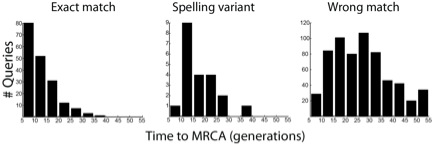
\includegraphics[width=0.65\textwidth]{Figures/App1/SuppFig1.jpg}
\end{figure}
\textbf{The TMRCA profiles of haplotype queries.} Records that matched exactly the input surname (left) showed a geometric-like distribution. For most records with a minute spelling variant from the original surname (center) the  MRCA was 10-15 generations ago. Wrong matches (right) mainly showed an ancient MRCA.

\pagebreak
\subsection{Supplemental Figure 2}
\begin{figure}[h!]
\centering
\label{fig:sursup2}
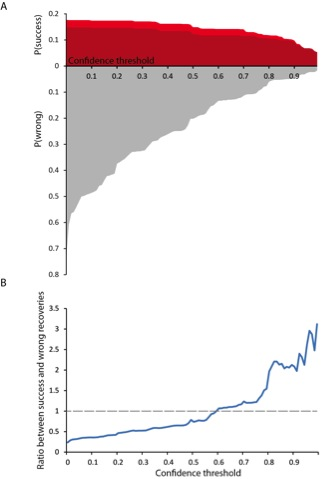
\includegraphics[width=0.4\textwidth]{Figures/App1/SuppFig2.jpg}
\end{figure}
\textbf{Performance of surname recovery at different confidence thresholds.} \textbf{(A)} The rate of successful recovery with exact matches (dark red) and spelling variants (light red) versus the wrong recovery rate (gray) as a function of confidence threshold level. \textbf{(B)} The ratio between successful recoveries to wrong recoveries.

\pagebreak
\subsection{Supplemental Figure 3}
\begin{figure}[h!]
\centering
\label{fig:sursup3}
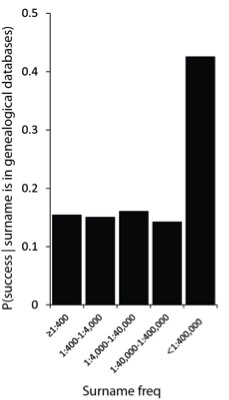
\includegraphics[width=0.4\textwidth]{Figures/App1/SuppFig3.jpg}
\end{figure}
\textbf{The probability of successful recovery given that the surname has at least one record in Ysearch or SMGF as a function of the surname frequency.}

\pagebreak
\subsection{Supplemental Figure 4}
\begin{figure}[h!]
\centering
\label{fig:sursup4}
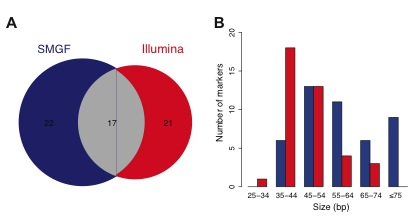
\includegraphics[width=0.65\textwidth]{Figures/App1/SuppFig4.jpg}
\end{figure}
\textbf{Comparison between Illumina Y-STR profiling and the Sorenson Genomics genetic genealogy service.} \textbf{(A)} Illumina profiling returned the results of 38 Y-STR markers. The genetic genealogy service uses a panel of 49 markers, 39 of which are included in lobSTR's Y-STR reference. The results of all 17 markers that were profiled by both strategies were identical. \textbf{(B)} The distribution of total STR region lengths is shown for the markers typed by Sorenson (blue) versus markers typed by lobSTR (red).

\pagebreak
\subsection{Supplemental Figure 5}
\begin{figure}[h!]
\centering
\label{fig:sursup5}
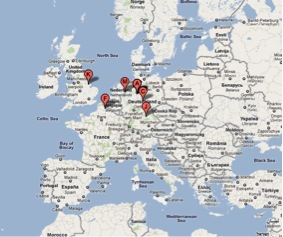
\includegraphics[width=0.65\textwidth]{Figures/App1/SuppFig5a.jpg}
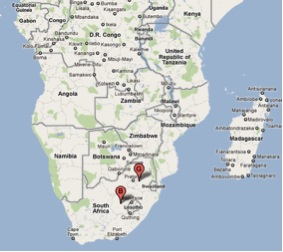
\includegraphics[width=0.65\textwidth]{Figures/App1/SuppFig5b.jpg}
\end{figure}
\textbf{Ancestral origins of Venter records in Ysearch}. The ancestral origin of the top match is labeled with an arrow.

\pagebreak
\subsection{Supplemental Figure 6}
\begin{figure}[h!]
\centering
\label{fig:sursup6}
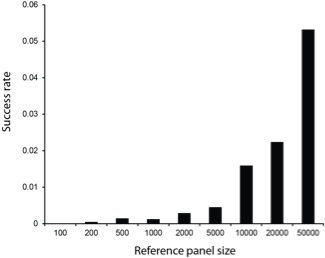
\includegraphics[width=0.65\textwidth]{Figures/App1/SuppFig6.jpg}
\end{figure}
\textbf{The estimated success rate for surname recovery after imputation as a function of the imputation panel size.}

\pagebreak
\section{Supplemental Tables}
\subsection{Supplemental Table 1}
\begin{figure}[h!]
\centering
\label{tab:sursuptab1} % even though we use a figure screenshot
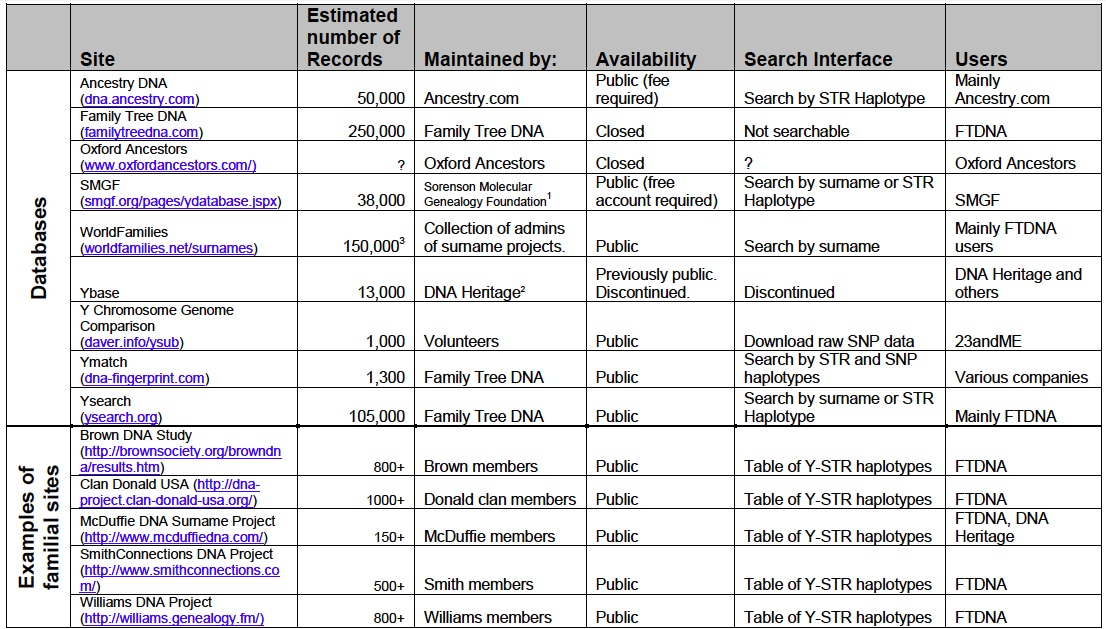
\includegraphics[width=0.95\textwidth]{Figures/App1/SuppTab1.jpg}
\end{figure}
List of major genetic genealogy sites that display Y chromosome and surname information. The top section lists genetic genealogy databases. The bottom section lists examples of privately maintained familial genetic genealogy sites.
$^1$ SMGF was recently acquired by Ancestry.com. $^2$ DNA Heritage was acquired by FamilyTreeDNA in 2011. $^3$ Includes only users whose surnames are present in the 2000 US Census.

\pagebreak
\subsection{Supplemental Table 2}
\begin{table}[h!]
\centering
\label{tab:sursuptab2}
\begin{adjustbox}{height=0.4\textheight}
\begin{tabular}{l l l l}
\hline
Marker & Expected mutation rate & Mean & $\sigma$ \\
\hline
DYS19     & 0.00437  & 14.34   & 0.8045 \\
DYS385a   & 0.00208  & 12.0869 & 1.6522 \\
DYS385b   & 0.00414  & 14.5464 & 1.449  \\
DYS388    & 0.000425 & 12.5142 & 1.0753 \\
DYS389a   & 0.00551  & 12.9668 & 0.6644 \\
DYS389b   & 0.00383  & 29.326  & 1.0418 \\
DYS390    & 0.00152  & 23.6032 & 1.0229 \\
DYS391    & 0.00323  & 10.4858 & 0.6104 \\
DYS392    & 0.00097  & 12.3413 & 1.1069 \\
DYS393    & 0.00211  & 13.0752 & 0.6025 \\
DYS426    & 0.000398 & 11.6459 & 0.5198 \\
DYS437    & 0.00153  & 14.9094 & 0.6931 \\
DYS438    & 0.000956 & 11.2206 & 1.0643 \\
DYS439    & 0.00384  & 11.66   & 0.8567 \\
DYS442    & 0.00978  & 17.2273 & 1.3301 \\
DYS444    & 0.00545  & 12.3666 & 0.892  \\
DYS445    & 0.00216  & 11.6015 & 0.9401 \\
DYS446    & 0.00267  & 13.1767 & 1.372  \\
DYS447    & 0.00212  & 24.6396 & 1.2057 \\
DYS448    & 0.000394 & 19.3437 & 0.8748 \\
DYS449    & 0.0122   & 29.5472 & 1.6474 \\
DYS452    & 0.00402  & 30.1854 & 1.1041 \\
DYS454    & 0.000475 & 11.0484 & 0.3744 \\
DYS455    & 0.000426 & 10.648  & 0.9704 \\
DYS456    & 0.00494  & 15.4571 & 1.1065 \\
DYS458    & 0.00836  & 16.6389 & 1.2634 \\
DYS459a   & 0.00013  & 8.753   & 0.5017 \\
DYS459b   & 0.00013  & 9.601   & 0.5422 \\
DYS460    & 0.00622  & 10.6976 & 0.639  \\
DYS461    & 0.000989 & 11.882  & 0.6914 \\
DYS462    & 0.00265  & 11.3571 & 0.6266 \\
DYS464a   & 0.00018  & 13.8555 & 1.4488 \\
DYS464b   & 0.00018  & 14.7374 & 1.0564 \\
DYS464c   & 0.00018  & 15.8236 & 1.124  \\
DYS464d   & 0.00018  & 16.5742 & 1.1157 \\
DYS635    & 0.00385  & 22.6604 & 1.1601 \\
GATA-A10  & 0.00332  & 15.5234 & 1.2242 \\
GATA-H4   & 0.00322  & 10.7333 & 0.7801 \\
GGAAT1B07 & 0.0024   & 10.2854 & 0.7397 \\
YCAIIa    & 0.002    & 19.0997 & 0.905  \\
YCAIIb    & 0.002    & 22.136  & 1.2624 \\
\hline
\end{tabular}
\end{adjustbox}
\caption{\textbf{List of markers used to challenge Ysearch and SMGF.} Mutation rates are based on Ballantyne et al. \cite{BallantyneGoedbloedFangEtAl2010}. YCAII was absent from this study and set to 0.002 according to Walsh \cite{Walsh2001}. Mean and standard deviations for marker values are calculated using Ysearch with NIST nomenclature.}
\end{table}

\pagebreak
\subsection{Supplemental Table 3}
\label{tab:sursuptab3}
\begin{tabularx}{\linewidth}{l l l l l l }
\hline
Marker & Start & End & Alt location & Ref allele & Motif structure \\
\hline
DYS394/19   & 9521989  & 9522052  &                        & 15 & {[}TAGA{]}3TAGG{[}TAGA{]}n                                                                                                           \\
DYS385a/b   & 20842518 & 20842573 & chrY:19260956-19261212 & 14 & {[}GAAA{]}n                                                                                                                          \\
DYS388      & 14747535 & 14747570 &                        & 12 & {[}ATT{]}n                                                                                                                           \\
DYS389I     & 14612191 & 14612238 &                        & 12 & {[}TCTG{]}m{[}TCTA{]}n                                                                                                               \\
DYS389B     & 14612338 & 14612405 &                        & 29 & {[}TCTG{]}m{[}TCTA{]}n                                                                                                               \\
DYS390      & 17274947 & 17275042 &                        & 24 & {[}TCTG{]}n{[}TCTA{]}m{[}TCTG{]}p{[}TCTA{]}q                                                                                         \\
DYS391      & 14102795 & 14102838 &                        & 11 & {[}TCTA{]}n                                                                                                                          \\
DYS392      & 22633873 & 22633911 &                        & 13 & {[}TAT{]}n                                                                                                                           \\
DYS393      & 3131152  & 3131199  &                        & 12 & {[}AGAT{]}n                                                                                                                          \\
DYS406S1    & 23843595 & 23843634 &                        & 10 & {[}TATC{]}n                                                                                                                          \\
DYS413a/b   & 16099088 & 16099133 & chrY:14676647-14676820 & 23 & {[}TG{]}n                                                                                                                            \\
DYS426      & 19134850 & 19134885 &                        & 12 & {[}GTT{]}n                                                                                                                           \\
DYS434      & 14466533 & 14466568 &                        & 9  & TAAT{[}CTAT{]}n                                                                                                                      \\
DYS435      & 14496298 & 14496333 &                        & 9  & {[}TGGA{]}n                                                                                                                          \\
DYS436      & 15203862 & 15203897 &                        & 12 & {[}GTT{]}n                                                                                                                           \\
DYS437      & 14466994 & 14467057 &                        & 16 & {[}TCTA{]}n{[}TCTG{]}2{[}TCTA{]}4                                                                                                    \\
DYS438      & 14937824 & 14937873 &                        & 10 & {[}TTTTC{]}n                                                                                                                         \\
DYS439      & 14515312 & 14515363 &                        & 13 & {[}GATA{]}n                                                                                                                          \\
DYS441      & 14981831 & 14981908 &                        & 16 & {[}TTCC{]}n                                                                                                                          \\
DYS442      & 14761103 & 14761168 &                        & 17 & {[}TATC{]}2{[}TGTC{]}3{[}TATC{]}n                                                                                                    \\
DYS444      & 19226192 & 19226247 &                        & 14 & {[}TAGA{]}n                                                                                                                          \\
DYS445      & 22092602 & 22092649 &                        & 12 & {[}TTTA{]}n                                                                                                                          \\
DYS446      & 3131458  & 3131527  &                        & 14 & {[}TCTCT{]}n                                                                                                                         \\
DYS447      & 15278740 & 15278854 &                        & 23 & {[}TAATA{]}n{[}TAAAA{]}1{[}TAATA{]}m{[}TAAAA{]}1{[}TAATA{]}p                                                                         \\
DYS448\_1   & 24365070 & 24365136 &                        & 11 & {[}AGAGAT{]}n                                                                                                                        \\
DYS448\_2   & 24365178 & 24365225 &                        & 8  & {[}AGAGAT{]}n                                                                                                                        \\
DYS449\_1   & 8218014  & 8218074  &                        & 13 & {[}TTTC{]}n                                                                                                                          \\
DYS449\_2   & 8218124  & 8218179  &                        & 14 & {[}TTTC{]}n                                                                                                                          \\
DYS450      & 8126300  & 8126344  &                        & 8  & {[}ATTTT{]}n                                                                                                                         \\
DYS452      & 21620478 & 21620632 &                        & 31 & {[}TATAC{]}m{[}TGTAC{]}n{[}TATAC{]}p{[}CATAC{]}{[}TATAC{]}{[}CATAC{]}{[}TATAC{]}q{[}CATAC{]}r{[}TATAC{]}s{[}CATAC{]}{[}TATAC{]}t     \\
DYS454      & 8224156  & 8224199  &                        & 11 & {[}AAAT{]}n                                                                                                                          \\
DYS455      & 6911569  & 6911612  &                        & 11 & {[}AAAT{]}n                                                                                                                          \\
DYS456      & 4270960  & 4271019  &                        & 15 & {[}AGAT{]}n                                                                                                                          \\
DYS458      & 7867880  & 7867943  &                        & 16 & {[}GAAA{]}n                                                                                                                          \\
DYS459a/b   & 26078851 & 26078890 & chrY:26292857-26293004 & 10 & {[}TAAA{]}n                                                                                                                          \\
DYS460      & 21050842 & 21050881 &                        & 10 & {[}ATAG{]}n                                                                                                                          \\
DYS461      & 21050690 & 21050737 &                        & 12 & {[}TAGA{]}n{[}CAGA{]}                                                                                                                \\
DYS462      & 21317047 & 21317090 &                        & 11 & {[}TATG{]}n                                                                                                                          \\
DYS463      & 7643509  & 7643628  &                        & 24 & {[}AAAGG{]}m {[}AAGGG{]}n {[}AAGGA{]}p                                                                                               \\
DYS472      & 16508484 & 16508507 &                        & 8  & {[}AAT{]}n                                                                                                                           \\
DYS481      & 8426378  & 8426443  &                        & 22 & {[}CTT{]}n                                                                                                                           \\
DYS485      & 22099634 & 22099681 &                        & 16 & {[}TTA{]}n                                                                                                                           \\
DYS487      & 8914174  & 8914212  &                        & 13 & {[}TTA{]}n                                                                                                                           \\
DYS490      & 3443765  & 3443800  &                        & 12 & {[}TTA{]}n                                                                                                                           \\
DYS492      & 17414337 & 17414369 &                        & 12 & {[}ATT{]}n                                                                                                                           \\
DYS494      & 21386168 & 21386197 &                        & 10 & {[}TTA{]}n                                                                                                                           \\
DYS495      & 15011300 & 15011346 &                        & 15 & {[}AAT{]}n                                                                                                                           \\
DYS505      & 3640831  & 3640878  &                        & 12 & {[}TCCT{]}n                                                                                                                          \\
DYS511      & 17304923 & 17304958 &                        & 10 & {[}GATA{]}n                                                                                                                          \\
DYS520      & 7730432  & 7730511  &                        & 20 & {[}ATAG{]}n{[}ATAC{]}n                                                                                                               \\
DYS522      & 7415625  & 7415664  &                        & 10 & {[}GATA{]}n                                                                                                                          \\
DYS531      & 8466195  & 8466238  &                        & 11 & {[}AAAT{]}n                                                                                                                          \\
DYS533      & 18393226 & 18393273 &                        & 12 & {[}ATCT{]}n                                                                                                                          \\
DYS634      & 18392976 & 18393035 &                        & 15 & {[}CTTT{]}n                                                                                                                          \\
DYS537      & 19358850 & 19358889 &                        & 10 & {[}TCTA{]}n                                                                                                                          \\
DYS549      & 21520224 & 21520275 &                        & 13 & {[}GATA{]}n                                                                                                                          \\
DYS556      & 22601453 & 22601496 &                        & 11 & {[}AATA{]}n                                                                                                                          \\
DYS557      & 23234712 & 23234775 &                        & 16 & {[}TTTC{]}n                                                                                                                          \\
DYS565      & 16526732 & 16526775 &                        & 12 & {[}ATAA{]}n                                                                                                                          \\
DYS568      & 8822555  & 8822594  &                        & 11 & {[}AAAT{]}n                                                                                                                          \\
DYS570      & 6861231  & 6861298  &                        & 17 & {[}TTTC{]}n                                                                                                                          \\
DYS572      & 3679660  & 3679699  &                        & 10 & {[}AAAT{]}n                                                                                                                          \\
DYS575      & 7436257  & 7436296  &                        & 10 & {[}AAAT{]}n                                                                                                                          \\
DYS576      & 7053359  & 7053426  &                        & 16 & {[}AAAG{]}n                                                                                                                          \\
DYS578      & 22562564 & 22562599 &                        & 9  & {[}AAAT{]}n                                                                                                                          \\
DYS589      & 24485693 & 24485757 &                        & 12 & {[}TTTTA{]}n                                                                                                                         \\
DYS590      & 8555980  & 8556019  &                        & 8  & {[}TTTTG{]}n                                                                                                                         \\
DYS594      & 21656837 & 21656886 &                        & 10 & {[}AAATA{]}n                                                                                                                         \\
DYS607      & 18414382 & 18414457 &                        & 19 & {[}GAAG{]}n{[}GAAA{]}{[}GAAG{]}{[}GAAA{]}{[}GAAG{]}                                                                                  \\
DYS617      & 19081518 & 19081553 &                        & 12 & {[}TTAn{]}                                                                                                                           \\
DYS635      & 14379564 & 14379655 &                        & 23 & {[}TCTA{]}4{[}TGTA{]}2{[}TCTA{]}2{[}TGTA{]}2{[}TCTA{]}2{[}TGTA{]}m{[}TCTA{]}n                                                        \\
DYS636      & 22634857 & 22634900 &                        & 12 & {[}ATTT{]}n                                                                                                                          \\
DYS638      & 17645491 & 17645534 &                        & 11 & {[}TTTA{]}n                                                                                                                          \\
DYS641      & 16134296 & 16134335 &                        & 10 & {[}TAAA{]}n                                                                                                                          \\
DYS643      & 17426012 & 17426066 &                        & 11 & {[}CTTTT{]}n                                                                                                                         \\
DYS714      & 22147731 & 22147865 &                        & 27 & {[}TTTCT{]}m{[}CTTCT{]}n{[}TTTCT{]}p{[}CTTCT{]}q{[}TTTCT{]}r                                                                         \\
DYS717      & 17313245 & 17313324 &                        & 16 & {[}GTACT{]}m {[}GTATT{]}n                                                                                                            \\
GATA-A10    & 18718879 & 18718938 &                        & 15 & {[}TCCA{]}2 {[}TATC{]}n                                                                                                              \\
GATA-H4     & 18743553 & 18743600 &                        & 12 & {[}TAGA{]}n                                                                                                                          \\
YCAIIa/b    & 19622111 & 19622156 & chrY:19016986-19017135 & 23 & {[}CA{]}n                                                                                                                            \\
DYS395S1a/b & 19739341 & 19739381 & chrY:18899736-18899977 & 15 & {[}AAC{]}n                                                                                                                           \\
DYS716      & 13140129 & 13140274 &                        & 28 & {[}ACTCGC{]}{[}ACTCC{]}m{[}ATTCC{]}n{[}TATTCTATTGA{]}{[}ACTCC{]}{[}ATTCC{]}{[}ACTCC{]}2{[}ATTCA{]}{[}ATTCC{]}2{[}ACTTC{]}{[}ATTCC{]} \\
\hline
\end{tabularx}
\textbf{Y-STR genomic locations and conventions.} All coordinates are given for human genome build hg19. Conventions follow NIST guidelines whenever available. $^*$ The values for DYS448 and DYS449 were determined by adding the alleles typed at DYS448\_1/DYS448\_2 and DYS449\_1/DYS449\_2. The complete repeat structures for DYS448 and DYS449 are  [AGAGAT]mN42[AGAGAT]n and [TTTC]m [N]50 [TTTC]n, respectively.

\pagebreak
\subsection{Supplemental Table 4}
\label{tab:sursuptab4}
\begin{tabularx}{\linewidth}{l l l l}
\hline
Marker & Craig Venter & Best Ysearch hit (VPBT4) \\
\hline
DYS388    & 12 & 12 \\
DYS391    & 10 & 10 \\
DYS392    & 13 & 13 \\
DYS395S1a & 15 & 15 \\
DYS395S1b & 16 & 16 \\
DYS413a   & 23 & 23 \\
DYS426    & 12 & 12 \\
DYS436    & 12 & 12 \\
DYS438    & 12 & 12 \\
DYS439    & 12 & 12 \\
DYS442    & 12 & 12 \\
DYS450    & 8  & 8  \\
DYS454    & 11 & 11 \\
DYS455    & 11 & 11 \\
DYS458    & 17 & 17 \\
DYS459a   & 9  & 9  \\
DYS461    & 12 &    \\
DYS462    & 11 &    \\
DYS472    & 8  & 8  \\
DYS481    & 22 & 22 \\
DYS485    & 16 &    \\
DYS492    & 13 & 13 \\
DYS494    & 9  &    \\
DYS531    & 12 & 12 \\
DYS534    & 16 & 16 \\
DYS537    & 10 & 10 \\
DYS549    & 12 &    \\
DYS556    & 11 &    \\
DYS557    & 16 & 16 \\
DYS565    & 12 & 12 \\
DYS568    & 11 & 11 \\
DYS570    & 17 & 17 \\
DYS578    & 9  & 9  \\
DYS590    & 9  & 9  \\
DYS594    & 10 & 10 \\
DYS617    & 12 & 12 \\
DYS636    & 12 &    \\
DYS638    & 11 &    \\
DYS641    & 10 & 10 \\
DYS714    & 25 & 25 \\
YCAIIa    & 19 & 19 \\
YCAIIb    & 23 & 23 \\
\hline
\end{tabularx}
\textbf{Craig Venter's haplotype from his personal genome versus the best Ysearch match.} Only Ysearch markers with corresponding sequencing results are shown. All alleles are reported using FamilyTreeDNA nomenclature to match the Ysearch convention. For Genebank read accessions, see Supplemental Material at \url{http://www.sciencemag.org/content/339/6117/321/suppl/DC1}.

\pagebreak
\subsection{Supplemental Table 5}
\begin{table}[h!]
\centering
\label{tab:sursuptab5}
\begin{adjustbox}{width=1\textwidth}
\begin{tabular}{l l l}
\hline
User surname & Ancestor surname & Origin \\
\hline
Venter & Von Dempter  & Hameln, Germany                                 \\
Venter & Venter       & Bloemfontein, South Africa                      \\
Venter & Venter       & Germany                                         \\
Venter & von Dempter  & Hamelin, Lower Saxony/Niedersachsen, Germany    \\
Venter & Von Dempter  & Hameln, Lower Saxony/Niedersachsen, Germany     \\
Venter & Venter       & Hamel, France                                   \\
Venter & Venter       & Witbank, South Africa                           \\
Venter & Von Dempter  & Hameln, Germany                                 \\
Venter & Venter       & Hamln, Germany                                  \\
Venter & Venter       & Roth near Meisenheim, Palatinate/Pfalz, Germany \\
Venter &              & Lincolnshire, England                           \\
Venter & Venter       & Hameln, Lower Saxony/Niedersachsen, Germany     \\
Venter & van Deventer & Oldenzee, Netherlands              \\
\hline
\end{tabular}
\end{adjustbox}
\caption{\textbf{Venter records in Ysearch and their ancestral origins.} In red - the top match to Craig Venter's Genome.}
\end{table}

%% This defines the bibliography file (main.bib) and the bibliography style.
%% If you want to create a bibliography file by hand, change the contents of
%% this file to a `thebibliography' environment.  For more information 
%% see section 4.3 of the LaTeX manual.
\begin{singlespace}
\bibliographystyle{plain}
\bibliography{MGymrekRefs}
\end{singlespace}

\end{document}

